%%%%%%%%%%%%%%%
% MSc Thesis — York University, Department of Electrical Engineering and Computer Science
%
% Formatting is inherited from an accepted York EECS MSc thesis template
% (Yasaman Parhizkar's adaptation of Manvi Agarwal's Groningen template).
% FGS does not publish an official LaTeX class; this template is the working authority.
%
% Author: Shayan Mohammadizadehsamakosh
%%%%%%%%%%%%%%%

\documentclass[letterpaper,11pt]{article}

% ---- Core packages (inherited from the York template) ----
\usepackage{setspace}
\usepackage{comment}
\usepackage{multirow}
\usepackage[font=small]{caption}
\usepackage{subcaption}
\usepackage{xcolor}
\usepackage{color}
\usepackage{amsmath}
\usepackage{booktabs}
\usepackage{amssymb}
\usepackage{wrapfig}    % inline figures
\usepackage{enumitem}
\usepackage{graphicx}   % images
\usepackage{here}       % forced figure placement
\usepackage{pslatex}    % PostScript fonts
\usepackage{fancyhdr}
\usepackage{float}
% [numbers] is required: \bibliographystyle{ieeetr} is a numeric style, and
% natbib's default author-year mode errors out against it.
\usepackage[numbers]{natbib}
\usepackage[nottoc,notlof]{tocbibind}
\usepackage{pifont}     % \ding
\newcommand{\cmark}{\ding{51}}   % check mark
\newcommand{\xmark}{\ding{55}}   % cross mark

\usepackage{tcolorbox}  % boxed environments (prompt templates)
\tcbuselibrary{listings, breakable, skins}
\usepackage[hidelinks]{hyperref}
\usepackage{tocloft}
\usepackage{titlesec}
\usepackage{fmtcount}
\usepackage{etoolbox}
\usepackage{titletoc}

% ---- Additional packages carried over from the paper source ----
\usepackage[T1]{fontenc}
\usepackage{url}
\usepackage{amsfonts}
\usepackage{nicefrac}
\usepackage{microtype}
\usepackage{xspace}
\usepackage{afterpage}
\usepackage{courier}
\usepackage[table]{xcolor}
\usepackage{algorithm}
\usepackage{algpseudocode}
\usepackage{listings}

% ---- Geometry: equal margins ----
\usepackage[
	top    = 25mm,
	bottom = 25mm,
	left   = 25mm,
	right  = 25mm]{geometry}

% The template suppresses paragraph indentation. Typographically a paragraph break
% must be marked by either an indent or vertical space, so with \parindent at 0pt a
% \parskip is required -- without it consecutive paragraphs run together and the
% structure of the argument becomes invisible. The rubber component lets the page
% breaker absorb slack rather than leaving short pages.
\setlength{\parindent}{0pt}
\setlength{\parskip}{0.55\baselineskip plus 0.2\baselineskip minus 0.1\baselineskip}
% Keep lists tight so the added \parskip does not make them sprawl.
\setlist{topsep=0.25\baselineskip, itemsep=0.15\baselineskip, parsep=0pt}
\renewcommand{\refname}{Bibliography}
\graphicspath{{images/}{images/paper/}{images/new/}}
%%%%%%%%%%%%%%%
% Macro definitions.
%
% Base set inherited from the York EECS thesis template, with one correction:
% the original redefined single letters that collide with real LaTeX text-mode
% commands (accents \b \c \d \H \i \j \k \r \t \u \v and symbols \l \L \o \O \P \S).
% Those are commented out below. The collision is not hypothetical -- biblio.bib
% line 330 contains "C{\'\i}an" (Cian Hughes, MedGemma), which \def\i would break.
% This thesis writes v, q, y in plain italic anyway, matching the paper.
%%%%%%%%%%%%%%%

\def\0{{\mathbf 0}}
\def\1{{\mathbf 1}}

% --- Bold lowercase vectors (collision-free subset) ---
\def\e{{\mathbf e}}
\def\f{{\mathbf f}}
\def\g{{\mathbf g}}
\def\h{{\mathbf h}}
\def\m{{\mathbf m}}
\def\n{{\mathbf n}}
\def\p{{\mathbf p}}
\def\q{{\mathbf q}}
\def\s{{\mathbf s}}
\def\w{{\mathbf w}}
\def\x{{\mathbf x}}
\def\y{{\mathbf y}}
\def\z{{\mathbf z}}

% DISABLED -- these clobber LaTeX text-mode accents/symbols:
% \a \b \c \d \i \j \k \l \o \r \t \u \v
% Use \mathbf{v} etc. explicitly where a bold form is genuinely needed.

% --- Bold uppercase matrices (collision-free subset) ---
\def\A{{\mathbf A}}
\def\B{{\mathbf B}}
\def\C{{\mathbf C}}
\def\D{{\mathbf D}}
\def\E{{\mathbf E}}
\def\F{{\mathbf F}}
\def\G{{\mathbf G}}
\def\I{{\mathbf I}}
\def\J{{\mathbf J}}
\def\K{{\mathbf K}}
\def\M{{\mathbf M}}
\def\N{{\mathbf N}}
\def\Q{{\mathbf Q}}
\def\R{{\mathbf R}}
\def\T{{\mathbf T}}
\def\U{{\mathbf U}}
\def\V{{\mathbf V}}
\def\W{{\mathbf W}}
\def\X{{\mathbf X}}
\def\Y{{\mathbf Y}}
\def\Z{{\mathbf Z}}
% DISABLED: \H \L \O \P \S (text-mode symbols/accents)

\def\rE{{\text{E}}}
\def\rPr{{\text{Pr}}}
\def\Tr{{\text{Tr}}}
\def\ie{{\textit{i.e.}}}
\def\eg{{\textit{e.g.}}}

% --- Calligraphic sets ---
\def\cA{{\mathcal A}}
\def\cB{{\mathcal B}}
\def\cC{{\mathcal C}}
\def\cD{{\mathcal D}}
\def\cE{{\mathcal E}}
\def\cF{{\mathcal F}}
\def\cG{{\mathcal G}}
\def\cH{{\mathcal H}}
\def\cI{{\mathcal I}}
\def\cK{{\mathcal K}}
\def\cL{{\mathcal L}}
\def\cM{{\mathcal M}}
\def\cN{{\mathcal N}}
\def\cO{{\mathcal O}}
\def\cP{{\mathcal P}}
\def\cQ{{\mathcal Q}}
\def\cR{{\mathcal R}}
\def\cS{{\mathcal S}}
\def\cT{{\mathcal T}}
\def\cU{{\mathcal U}}
\def\cV{{\mathcal V}}
\def\cW{{\mathcal W}}
\def\cX{{\mathcal X}}
\def\cY{{\mathcal Y}}
\def\cZ{{\mathcal Z}}

% --- Bold greek ---
\def\bpi{{\pmb{\pi}}}
\def\bphi{{\pmb{\phi}}}
\def\bpsi{{\pmb{\psi}}}
\def\balpha{{\boldsymbol \alpha}}
\def\bbeta{{\boldsymbol \beta}}
\def\bmu{{\boldsymbol \mu}}
\def\btheta{{\boldsymbol \theta}}
\def\bupsilon{{\pmb{\upsilon}}}
\def\bvarphi{{\boldsymbol \varphi}}
\def\bLambda{{\boldsymbol \Lambda}}
\def\bPhi{{\boldsymbol \Phi}}
\def\bSigma{{\boldsymbol \Sigma}}

\def\bcdot{{\;\boldsymbol{\cdot}\;}}

\newcommand{\red}[1] {\textcolor[rgb]{1.0,0.0,0.0}{{#1}}}
\newcommand{\green}[1] {\textcolor[rgb]{0.0,0.75,0.0}{{#1}}}
\newcommand{\blue}[1] {\textcolor[rgb]{0.0,0.0,1.0}{{#1}}}

%%%%%%%%%%%%%%%
% Thesis-specific macros
%%%%%%%%%%%%%%%

% Title-page metadata (single place to edit)
\newcommand{\thesisdate}{August 2026}
\newcommand{\thesisyear}{2026}

% Method name, carried over from the paper source
\newcommand{\ourloss}{{\textsc{FiRe-MPO}}\xspace}

% Policy / reference model shorthands
\newcommand{\pit}{\pi_{\theta}}
\newcommand{\piref}{\pi_{\text{ref}}}
\newcommand{\KL}{\mathbb{D}_{\text{KL}}}

%%%%%%%%%%%%%%%
% Draft placeholder machinery.
% Flip \drafttrue -> \draftfalse for the submission build: every red box
% disappears, \tbdnum cells collapse to an em dash, and the outstanding-items
% page in main.tex is suppressed.
%%%%%%%%%%%%%%%
\newif\ifdraft \draftfalse

\usepackage[colorinlistoftodos,textsize=footnotesize,textwidth=\marginparwidth]{todonotes}

% Prose-level gap: renders as an inline red box, and is listed by \listoftodos.
\newcommand{\tbd}[1]{\ifdraft\todo[inline,color=red!25]{\textbf{TBD:} #1}\fi}

% Table-cell gap: renders as a red bracketed label in draft, an em dash in final.
\newcommand{\tbdnum}[1]{\ifdraft\textcolor{red}{\textbf{[#1]}}\else--\fi}


\definecolor{darkgreen}{rgb}{0.0, 0.5, 0.0}
\definecolor{darkred}{rgb}{0.5, 0.0, 0.0}
\definecolor{boxgray}{RGB}{240, 240, 240}

% ---- A numbered \subsubsubsection level under \subsubsection ----
\titleclass{\subsubsubsection}{straight}[\subsubsection]
\newcounter{subsubsubsection}[subsubsection]
\renewcommand\thesubsubsubsection{\thesubsubsection.\arabic{subsubsubsection}}
\titleformat{\subsubsubsection}
  {\normalfont\normalsize\bfseries}
  {\thesubsubsubsection}{1em}{}
\titlespacing*{\subsubsubsection}
  {0pt}{3.25ex plus 1ex minus .2ex}{1.5ex plus .2ex}

\setcounter{secnumdepth}{4}
\setcounter{tocdepth}{4}

\onehalfspacing
\begin{document}

\setcounter{secnumdepth}{4}
\setcounter{tocdepth}{4}

\pagenumbering{roman}
\begin{center}
    % Institutional logos. Drop the two files into images/logos/ as
    % lassonde.png and yorku.png (PDF or JPG also work -- adjust the extension
    % below). \IfFileExists guards the build so the title page still typesets
    % if they are absent.
    \vspace*{0.5cm}
    \IfFileExists{images/logos/lassonde.png}{%
      \raisebox{-0.5\height}{
\includegraphics[height=1.5cm]{images/logos/lassonde.png}}%
      \hspace{1.2cm}%
    }{}%
    \IfFileExists{images/logos/yorku.png}{%
      \raisebox{-0.5\height}{
\includegraphics[height=1.5cm]{images/logos/yorku.png}}%
    }{}%
    \par
    \vspace{2.5cm}
    {\bf{\Large Analyzing and Improving Fine-grained Preference\\[0.3cm]
    Optimization in Medical Vision-Language Models}}\\
    \vspace{1cm}{\bf \large Shayan Mohammadizadehsamakosh}\\
    \vspace{2cm}{\bf A Thesis Submitted to the Faculty of Graduate Studies\\
    In Partial Fulfillment of the Requirements\\
    for the Degree of Master of Science}\\
    \vspace{0.5cm}{\bf Graduate Program in Computer Science}\\
    \vspace{2cm} {\bf {\large York University}}\\
    {\bf {\large Toronto, Ontario}}\\
    \vspace{2cm} {\textbf{\thesisdate}}\\
    {\bf \copyright Shayan Mohammadizadehsamakosh, \thesisyear}
\end{center}
\thispagestyle{empty}

\newpage
\addtocontents{toc}{~\hfill\textbf{Page}\par}
\addcontentsline{toc}{section}{Abstract}
\textbf{Abstract}\\

Large Vision-Language Models (LVLMs) have achieved strong performance across medical imaging tasks, yet they remain prone to factual inconsistencies, poor visual grounding, and misalignment with clinically meaningful feedback. Among the post-training remedies proposed for these failures, Direct Preference Optimization (DPO) has been widely adopted for its ability to learn from comparisons without an explicit reward model. This thesis argues that its standard formulation is nonetheless structurally mismatched to clinical use in three ways. First, its sequence-level reward treats a diagnostically decisive span such as an anatomical side or a lesion attribute exactly like generic filler text, so the training signal is dominated by tokens that carry no clinical meaning. Second, because expert preference annotation is expensive, practitioners substitute the supervised fine-tuning reference as the preferred response; the resulting off-policy distribution shift lets the model raise its preference margin by imitating the reference's brevity and formatting rather than by correcting the clinical error, a failure mode we characterize as \emph{stylistic reward hacking}. Third, existing objectives contain no explicit visual grounding constraint, leaving models insensitive to the subtle pathological features that determine a diagnosis.

This thesis introduces \ourloss{}, a fine-grained, on-policy alignment framework built around three corresponding components. Preference pairs are constructed by minimally editing the model's own generations, correcting only clinically erroneous spans while preserving the original linguistic style, so the learning signal isolates factuality from surface form. A bidirectional token-wise KL regularizer balances the mean-seeking behaviour of forward KL, which preserves the base model's linguistic coverage, against the mode-seeking tail suppression of reverse KL, which is what prevents spuriously fluent but incorrect tokens. A visual-contrastive grounding objective pairs each image with a lesion-corrupted counterpart and reverses the preference direction when the supporting evidence has been removed, penalizing answers that are correct for the wrong reasons.

Across two state-of-the-art backbones and three clinical benchmarks spanning visual question answering and radiology report generation, \ourloss{} improves on both standard DPO and prior fine-grained alignment methods, with an average relative gain of $10.24\%$. Layer-wise attention analysis shows that the aligned models attend more consistently to diagnostically relevant image regions, and controlled ablations isolate the contribution of each component: the bidirectional regularizer, lesion-targeted rather than global image corruption, and on-policy rather than reference-style preference pairs.

\newpage
\section*{Acknowledgements}
\addcontentsline{toc}{section}{Acknowledgements}

I would like to express my deepest gratitude to my supervisor, Dr.~Elham Dolatabadi. Her guidance shaped this work at every stage, from the initial question of why preference optimization behaves differently in clinical settings to the framing of the analysis that became its central argument. I am grateful for her patience with the directions that did not work out, for her insistence on evidence over intuition whenever I was tempted to settle for the latter, and for the encouragement she offered at exactly the moments it was needed. Whatever rigour this thesis has, it owes to her supervision.

To my parents, Shayesteh Mehri and Samad Mohammadizadehsamakosh: this thesis exists because of you. You supported an education that took me far from home, across a distance measured in more than kilometres, and you did so without hesitation and without ever making me feel the cost of it. You taught me to be curious before you taught me anything else, and to finish what I start. Thank you for your patience through the long silences of a graduate degree, for your encouragement across every time zone, and for a confidence in me that I have not always shared. I am more grateful than these few lines can carry.

% ---- Table of Contents formatting ----
\setcounter{tocdepth}{2}

% Sections (top level) => "Chapter One: <Title> .... page"
\titlecontents{section}
  [0em]
  {\bfseries}
  {\ifx\thecontentslabel\empty
      % unnumbered (e.g., Abstract) -> no "Chapter"
      %
    \else
      Chapter~\Numberstringnum{\thecontentslabel}:~
    \fi}
  {}
  {\titlerule*[1pc]{.}\contentspage}
  []

% Subsections => "2.1 <Title> .... page" (no "Chapter")
\titlecontents{subsection}
  [2.5em]
  {}
  {\thecontentslabel\quad}
  {}
  {\titlerule*[1pc]{.}\contentspage}
  []

% --- Table of Contents ---
\newpage
\makeatletter
\renewcommand{\tableofcontents}{%
  \cleardoublepage
  \phantomsection
  \begin{center}
    {\bfseries\MakeUppercase{Table of Contents}}
  \end{center}
  \vspace{1.25em}
  \@starttoc{toc}
}
\makeatother
\tableofcontents

% --- List of Tables ---
\newpage
\makeatletter
\renewcommand{\listoftables}{%
  \cleardoublepage
  \section*{\centering {\large \MakeUppercase{List of Tables}}}%
  \vspace{1em}%
  \@starttoc{lot}%
}
\makeatother

\makeatletter
\renewcommand{\l@table}[2]{%
  \begingroup
    \def\numberline##1{Table~##1:\ }%
    \@dottedtocline{1}{0em}{3.8em}{#1}{#2}%
  \endgroup
}
\makeatother
\listoftables

% --- List of Figures ---
\newpage
\makeatletter
\renewcommand{\listoffigures}{%
  \cleardoublepage
  \section*{\centering {\large \MakeUppercase{List of Figures}}}%
  \vspace{1em}%
  \@starttoc{lof}%
}

\renewcommand{\l@figure}[2]{%
  \begingroup
    \def\numberline##1{Figure~##1:\ }%
    \@dottedtocline{1}{0em}{4em}{#1}{#2}%
  \endgroup
}
\makeatother

\listoffigures


\ifdraft
\newpage
\listoftodos[\textbf{Outstanding Items (draft only)}]
\fi

\newpage
\pagenumbering{arabic}
\section{Introduction}
\label{section:introduction}

\subsection{Motivation}
\label{sec:intro:motivation}

Large Vision-Language Models (LVLMs) have shown growing capabilities in perceiving and synthesizing visual and textual information, with rapid progress across general-purpose~\cite{bai2025qwen3, achiam2023gpt, singh2025openai, liu2024deepseek} and medical~\cite{li2024llavamed, chen2024chexagent, chen2024towards, sellergren2025medgemma, alsaad2024multimodal, saab2024capabilities} domains. A model that can read a chest radiograph and produce a structured report, or answer a clinician's question about a CT slice, is an obvious candidate for relieving pressure on radiology workflows and for extending access to imaging expertise in settings where a specialist is not available.

In high-stakes settings such as healthcare, however, LVLMs continue to exhibit unintended failure modes. They hallucinate clinical findings that are not present in the image, produce responses that are linguistically fluent yet factually unsupported by the underlying visual evidence~\cite{zhang2024medihall, seth2025hallucinogen}, and fail to reliably follow clinician instructions~\cite{vadlapati2026ai, xia2024cares}. These failures undermine medical reliability and limit safe deployment in real-world clinical workflows.

What makes these failures difficult is not their frequency but their form. Medical pretraining is highly effective at teaching a model the vocabulary, register, and structure of clinical text, so a hallucinated finding arrives phrased exactly as a radiologist would phrase it, hedged in the appropriate places and embedded in an otherwise accurate description. The error is confined to the few words that carry the diagnosis. This is a worse failure mode than incoherence would be, because fluency and confidence are the cues a human reader ordinarily uses to gauge reliability, and here they have been decoupled from correctness.

A related and equally serious problem is invisible at the level of the output altogether: a model may produce the correct answer for reasons that have nothing to do with the image, relying on the base rate of a finding or the anatomical default for a modality. Such an answer is indistinguishable from a well-grounded one when read, but it will fail on the atypical case --- which is precisely the case where a clinician most needs help. This failure is also self-concealing under standard evaluation: a model exploiting the base rates of its training distribution will score well on a test set drawn from the same distribution, and the deficit surfaces only on the rare presentations that aggregate accuracy barely registers.

Both problems share a structure worth naming at the outset. The model's output distribution is well-formed but incorrectly conditioned: it has learned what a good answer looks like without having learned what makes a superficially identical answer wrong. Supervised fine-tuning cannot easily repair this, because a demonstration exhibits only the correct answer and never the near-miss that must be rejected. Preference-based post-training is attractive precisely because a preference pair carries the information a demonstration lacks --- a negative example close enough to the positive one to isolate the distinction that matters.

\begin{figure}[t]
    \centering
    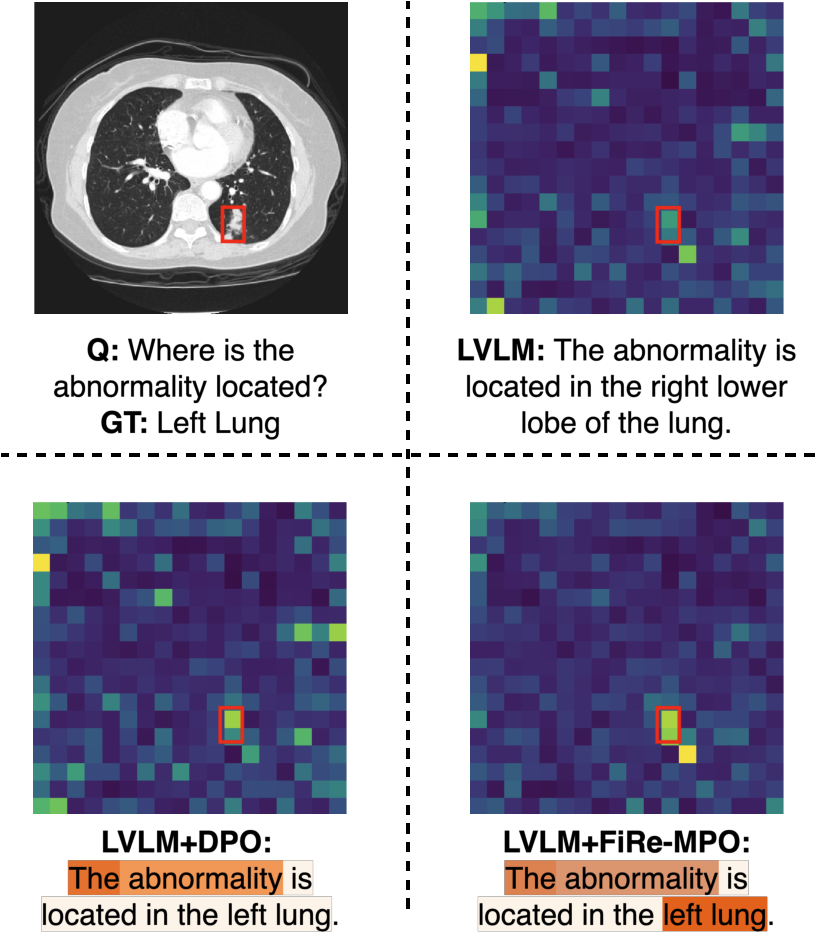
\includegraphics[width=0.75\textwidth]{generations.pdf}
    \caption{Reward assignment and visual attention in DPO versus \ourloss{}. DPO exhibits the same diffused visual attention as the base LVLM and fails to prioritize the reward of the clinically decisive words ``left lung'' (darker is higher).}
    \label{fig:framework_overview}
\end{figure}

\subsection{Preference Optimization and Its Clinical Mismatch}
\label{sec:intro:mismatch}

Beyond the initial supervised learning phase, post-training techniques have demonstrated remarkable success in refining model behaviour and improving task-specific performance~\cite{rafailov2023direct, ethayarajh2023kto, azar2024general}. Among them, Direct Preference Optimization (DPO) has gained popularity for its ability to skip explicit reward modeling~\cite{hein-etal-2025-chexalign, zhu2024mmedpo, savage2025fine, sun2024self}. Because it requires only comparisons between outputs rather than gold-standard demonstrations, it appears well suited to a domain where writing a reference answer requires a specialist but ranking two candidates does not.

This thesis argues that standard DPO and its variants face three critical limitations when applied to the medical domain, and that these limitations are not incidental but follow from the structure of the objective.

\emph{First}, the pairwise preference format is too coarse to capture the feedback clinicians actually provide, causing DPO-based approaches to yield inconsistent gains over supervised fine-tuning~\cite{kim2026benchmarking}. While clinical evaluation hinges on fine-grained correctness --- exact terminology, accurate anatomical localization --- standard DPO treats all response tokens uniformly during optimization. Consequently, diagnostically important spans such as findings, anatomical locations, and measurements contribute no more to the training signal than generic filler phrases such as ``the image shows'' or ``there is evidence of''. Figure~\ref{fig:framework_overview} shows this directly: the reward a DPO-aligned model assigns is spread evenly across the response, with the decisive words receiving no special weight.

\emph{Second}, because AI-generated preference labels are unreliable in medicine~\cite{delucia2026same, rankin2020reliability}, prior work substitutes the supervised fine-tuning ground truth as the preferred response~\cite{zhu2024mmedpo, liu2025rrg, savage2025fine}. This creates an off-policy distribution shift~\cite{yang2025mitigating}. Clinical reference answers are short and structured; model outputs are long and explanatory. The systematic stylistic gap between them becomes a spurious signal that the model exploits as a reward-hacking shortcut, optimizing stylistic patterns rather than clinical correctness. Because the preference objective is defined purely by the contrast between two responses, any property that separates them reliably will be learned --- and imitating a register is far easier than learning a diagnosis.

\emph{Third}, existing alignment objectives lack explicit visual grounding constraints, leaving models insensitive to subtle yet diagnostically decisive pathological features. Nothing in the objective distinguishes a correct answer read from the image from an identical answer produced by a linguistic prior. As Figure~\ref{fig:framework_overview} illustrates, DPO exhibits the same diffused visual attention as the unaligned base model even where it has corrected the answer.

Taken together these three limitations suggest that the inconsistent benefit of preference optimization in medicine is not a matter of insufficient tuning or insufficient data. Each is a consequence of a design decision that is sound in the general domain and unsound here, and each admits a specific remedy. That is the position this thesis develops and tests.

\subsection{Scope}
\label{sec:intro:scope}

Three boundaries are worth stating before the argument begins.

This thesis concerns \emph{post-training alignment}, not pretraining or architecture. The visual encoder and cross-modal projector of both backbones remain frozen throughout, and only the language model is adapted, using low-rank updates. One consequence is methodological rather than incidental: because the perceptual front end never changes, any improvement in visual grounding reported in Chapter~\ref{section:results} must be attributable to how the model \emph{uses} the visual representation rather than to a better representation, which makes the grounding claim cleaner than it would otherwise be. The corresponding cost is that errors rooted in perception rather than in verbalization are outside the reach of the method entirely.

The evaluation is confined to radiology --- two visual question answering datasets and one report generation dataset --- and is in-distribution, on the held-out test split of the corpus each model was aligned on. Whether the framework transfers to pathology, dermatology, or ophthalmology, whose visual grounding characteristics differ substantially, is left open, and is revisited in Section~\ref{sec:con:limitations}.

Finally, this work aims at factual and evidential correctness, not at clinical deployment. Nothing here addresses calibration, uncertainty communication, regulatory validation, or the human factors of how a clinician should incorporate model output into a decision. Improving factuality is a precondition for those questions rather than an answer to them, and Section~\ref{sec:con:impact} returns to the risk that improving surface quality alongside factuality can make residual errors harder, not easier, for a reader to catch.

\subsection{Thesis Statement and Research Questions}
\label{sec:intro:rqs}

\noindent\textbf{Thesis statement.} \emph{The inconsistent benefit of preference optimization for medical vision-language models is not a limitation of preference learning as such, but a consequence of three specific mismatches --- reward granularity, preference-pair construction, and the absence of a grounding constraint. Addressing all three jointly, within a single objective, yields consistent improvements in clinical factuality and in measured visual grounding across backbones and tasks.}

The thesis is organized around four research questions.

\begin{itemize}
    \item \textbf{RQ1.} Does the sequence-level reward of standard DPO fail to concentrate learning signal on the clinically decisive spans of a response, and does restricting the reward to those spans improve clinical correctness? \emph{(Sections~\ref{sec:ana:coarse}, \ref{sec:met:ranking}, \ref{sec:res:main}.)}

    \item \textbf{RQ2.} When the supervised reference is used as the preferred response, does the model optimize response style in preference to clinical correctness, and does constructing preference pairs from the model's own outputs remove this confound? \emph{(Sections~\ref{sec:ana:reward-hacking}, \ref{sec:met:data}, \ref{sec:res:dynamics}, \ref{sec:res:abl-style}.)}

    \item \textbf{RQ3.} How does the direction of the KL regularizer govern the trade-off between clinical precision and generative diversity, and is a bidirectional regularizer superior to either direction alone? \emph{(Sections~\ref{sec:ana:kl}, \ref{sec:met:kl}, \ref{sec:res:abl-kl}.)}

    \item \textbf{RQ4.} Can an explicit visual-contrastive objective, built on lesion-targeted rather than global image corruption, improve a model's reliance on diagnostically decisive image regions as measured inside the network? \emph{(Sections~\ref{sec:ana:grounding}, \ref{sec:met:corruption}, \ref{sec:res:grounding}, \ref{sec:res:abl-visual}.)}
\end{itemize}

\subsection{Contributions}
\label{sec:intro:contributions}

\begin{itemize}
    \item \textbf{An analysis of why preference optimization underperforms in clinical settings.} We characterize three failure modes --- coarse reward assignment, stylistic reward hacking, and the absence of grounding constraints --- and add a fourth axis of analysis in the geometry of the KL regularizer. We show that stylistic reward hacking is visible not only in downstream accuracy but in the optimization itself: an off-policy DPO run saturates its preference objective within a twelfth of an epoch, after which its gradients collapse by six orders of magnitude and training effectively halts.

    \item \textbf{A medical preference data framework.} We propose a strategy for generating on-policy preference datasets from existing medical SFT data. By creating counterfactual pairs that correct specific model hallucinations while preserving original syntax, we move beyond simple ground-truth comparisons to provide more precise supervision. The construction additionally produces lesion-targeted corrupted images by text-guided medical segmentation, giving a visual counterpart to each textual pair.

    \item \textbf{A multimodal fine-grained regularized loss.} We introduce \ourloss{}, a loss operating at both the text and image levels. It provides fine-grained medical rewards on clinically divergent spans, applies a bidirectional token-wise KL regularizer that balances coverage preservation against tail suppression, and adds a dual-constraint visual term that reverses the preference direction when the supporting evidence has been destroyed.

    \item \textbf{Empirical validation across backbones and tasks.} Experiments across medical VQA and report-generation benchmarks demonstrate that \ourloss{} consistently outperforms both standard DPO and RRPO, achieving an average relative improvement of $10.24\%$ across two state-of-the-art LVLMs, together with layer-wise evidence of improved visual grounding and controlled ablations isolating each component.
\end{itemize}

\subsection{Thesis Outline}
\label{sec:intro:outline}

Chapter~\ref{section:background} provides the technical background: the architecture of vision-language models, their medical specialization, the derivation of DPO from reinforcement learning from human feedback, the information-theoretic properties of the KL divergence in both directions, and the benchmarks and metrics used to evaluate clinical systems. Chapter~\ref{section:related} positions this work against the literature on fine-grained alignment, multimodal preference learning, and clinical preference optimization, closing with a comparison table.

Chapter~\ref{section:analysis} develops the analysis that motivates the method, treating each failure mode in turn and concluding with a set of design desiderata. Chapter~\ref{section:method} presents \ourloss{}: the on-policy preference construction pipeline, the lesion-targeted visual corruption procedure, the dual-constraint ranking loss, the bidirectional token-wise KL regularizer, and the implementation.

Chapter~\ref{section:setup} describes the experimental setup, including a characterization of the generated preference corpora. Chapter~\ref{section:results} reports the main results, the layer-wise grounding analysis, the training dynamics, and four ablations isolating the individual design choices. Chapter~\ref{section:conclusion} discusses what the results support, states the limitations of the study, addresses broader impact, and outlines future work.

\section{Background}
\label{section:background}

This chapter establishes the technical foundations on which the rest of the thesis rests. Section~\ref{sec:bg:lvlm} describes how large vision-language models are constructed and how they generate text conditioned on an image. Section~\ref{sec:bg:medical-lvlm} covers their adaptation to medicine and, importantly, the failure modes that domain pretraining does not remove. Section~\ref{sec:bg:alignment} develops the alignment pipeline from supervised fine-tuning through reinforcement learning from human feedback to Direct Preference Optimization, deriving the DPO objective in full because the structure of that derivation is what the analysis in Chapter~\ref{section:analysis} exploits. Section~\ref{sec:bg:dpo-variants} surveys the variants that address DPO's known weaknesses. Section~\ref{sec:bg:kl} develops the information-theoretic machinery needed to reason about the regularizer, and Section~\ref{sec:bg:benchmarks} describes the datasets and metrics used to evaluate clinical vision-language systems.

\subsection{Large Vision-Language Models}
\label{sec:bg:lvlm}

A large vision-language model (LVLM) is a system that accepts an interleaved sequence of images and text and produces text. Contemporary LVLMs are overwhelmingly built by composing three components that are pretrained separately and then connected: a visual encoder, a modality projector, and an autoregressive language model. Understanding this decomposition matters for this thesis because the alignment method developed in Chapter~\ref{section:method} modifies only the third component, and the interpretation of its grounding results depends on that fact.

\subsubsection{Visual Encoders and Modality Projection}

The visual encoder maps an input image to a sequence of continuous vectors. The dominant choice is a Vision Transformer (ViT)~\cite{dosovitskiy2021image}, which partitions the image into fixed-size patches, embeds each patch linearly, adds positional information, and processes the resulting sequence with the same self-attention architecture used for text~\cite{vaswani2017attention}. The output is one vector per patch, so an image becomes a sequence of \emph{visual tokens} whose length is determined by the image resolution and the patch size.

The quantities involved are worth making concrete, because they explain several practical constraints encountered later. At a patch size of $14$ or $16$ pixels, a $1024 \times 1024$ image yields on the order of four thousand patches before any merging. Architectures typically reduce this --- for instance by merging adjacent $2 \times 2$ patch groups into a single token --- but a single high-resolution medical image still occupies hundreds to low thousands of positions in the language model's context. Since attention cost grows quadratically in sequence length, and since the objective developed in this thesis requires several forward passes over image-bearing sequences per optimization step, the visual token count is the dominant term in both the memory and the time budget reported in Section~\ref{sec:met:implementation}.

Encoders are typically initialized from contrastive image-text pretraining, most influentially CLIP~\cite{radford2021learning}, which trains an image encoder and a text encoder jointly so that matched image-caption pairs receive high cosine similarity and mismatched pairs low similarity, over very large web corpora. The resulting visual representation is already aligned to language in a coarse, whole-image sense, which is why it transfers well as the perceptual front end of a generative model.

It is worth noting for later that this pretraining objective supervises \emph{global} correspondence between an image and a caption. The loss is computed on a single pooled embedding per image; nothing in it requires that individual regions be separable, or that a small region be represented distinctly from the background it sits in. This is a reasonable trade for natural images, where the caption usually describes the dominant object. It is a poor fit for medical imaging, where the diagnostically decisive feature may occupy a fraction of a percent of the frame and differ from healthy tissue in texture rather than shape. The difficulty that medical LVLMs have with fine-grained localization is therefore not purely a matter of insufficient medical data; it is partly inherited from the pretraining objective of the encoder itself.

Because the visual encoder and the language model were trained independently, their representation spaces do not coincide. A \emph{projector} bridges them. The simplest and still widely used design is a linear layer or a small multilayer perceptron mapping each visual token into the language model's embedding dimension, as in LLaVA~\cite{liu2023visual, liu2024improved}. More elaborate designs compress the visual sequence before injection: BLIP-2's Q-Former~\cite{li2023blip2} uses a fixed set of learned query vectors that cross-attend to the encoder output, producing a short, fixed-length summary regardless of image size, and Flamingo~\cite{alayrac2022flamingo} instead interleaves gated cross-attention layers throughout a frozen language model.

These designs trade capacity against cost in a way that matters for grounding. A linear projector preserves the spatial correspondence between visual tokens and image regions: token $i$ still derives from patch $i$, so attention paid to that token is attention paid to a known location. A learned-query bottleneck destroys this correspondence, since each output vector is a weighted mixture over the whole image. The attention-based grounding measurements described in Section~\ref{sec:bg:benchmarks} depend on the first property, and are therefore natural for the LLaVA-style architectures used in this thesis. The two backbones evaluated here sit at different points on the remaining spectrum: \texttt{HuatuoGPT-Vision-7B}~\cite{chen2024towards} follows the LLaVA-style projection design, while \texttt{Qwen3-VL-4B-Instruct}~\cite{bai2025qwen3} employs an adapter supporting dynamic, high-resolution inputs, so that the number of visual tokens varies with the input rather than being fixed.

\subsubsection{Autoregressive Generation over Interleaved Sequences}

Once projected, visual tokens are simply prepended to or interleaved with the text token embeddings, and the language model runs unmodified. The model defines a distribution over responses by the usual autoregressive factorization,
\begin{equation}\label{eq:autoregressive}
\pi_\theta(y \mid v, q) = \prod_{t=1}^{|y|} \pi_\theta(y_t \mid v, q, y_{<t}),
\end{equation}
where $v$ denotes the image, $q$ the text prompt, and $y$ the generated response.

Three consequences of Equation~\ref{eq:autoregressive} recur throughout this thesis.

First, the log-likelihood of a response is a \emph{sum} over token positions,
\begin{equation}\label{eq:logprob-sum}
\log \pi_\theta(y \mid v,q) = \sum_{t=1}^{|y|} \log \pi_\theta(y_t \mid v,q,y_{<t}).
\end{equation}
Any objective defined on sequence log-probabilities is therefore implicitly a sum of per-token quantities. This is what makes it possible --- and, as Chapter~\ref{section:analysis} argues, necessary --- to restrict such an objective to a subset of positions: a sum can be taken over an index set, whereas a genuinely sequence-level quantity could not be decomposed at all.

Second, longer responses accumulate more terms, so sequence-level quantities scale with length. A preference objective built on differences of log-probabilities will therefore see systematically larger magnitudes for long responses than short ones, independently of their content. This has direct consequences for gradient magnitudes and is one route by which response length becomes a confound.

Third, the image influences generation only through the attention that text positions pay to the visual token positions. There is no other pathway: once projected, visual tokens are ordinary sequence elements, and the only mechanism by which they can affect the distribution over $y_t$ is the attention operation. This is what makes attention over visual tokens a meaningful proxy for visual grounding, and it is the basis of the metrics described in Section~\ref{sec:bg:benchmarks}. It is also why a model can produce a correct answer with negligible visual attention --- the language model's priors alone may suffice --- which is the failure mode Section~\ref{sec:ana:grounding} is concerned with.

\subsubsection{Instruction Tuning}

A model trained only to predict the next token continues text; it does not answer questions. Instruction tuning closes this gap by supervised fine-tuning on a large collection of (instruction, response) pairs spanning many tasks, which induces the ability to follow instructions expressed in natural language, including for tasks not seen during tuning~\cite{wei2022finetuned}. Visual instruction tuning extends this to the multimodal case by constructing (image, instruction, response) triples, typically by prompting a strong text-only model with image annotations to synthesize plausible dialogues~\cite{liu2023visual, dai2023instructblip}.

Instruction tuning is the last stage that both backbones in this thesis have already undergone, and it is the starting point --- the reference policy $\pi_{\text{ref}}$ --- for everything that follows. Its limitation motivates the rest of this chapter. Supervised fine-tuning teaches the model to imitate the distribution of demonstrated responses, but it provides no mechanism for expressing that one response is \emph{better} than another. Where demonstrations are ambiguous, incomplete, or occasionally wrong, imitation reproduces those properties faithfully.

This limitation is particularly consequential for synthetically generated instruction data, which is how most multimodal instruction corpora are built. When a text-only model writes a dialogue about an image it cannot see, working only from annotations, the resulting response is fluent and well-formed by construction but its grounding in the image is only as good as the annotation. A model trained to imitate such data learns the register of grounded description without necessarily learning the grounding, which is precisely the dissociation between surface form and evidential support that this thesis is about.

\subsection{Medical Vision-Language Models}
\label{sec:bg:medical-lvlm}

\subsubsection{Domain-Specialized Pretraining}

General-purpose LVLMs perform poorly on medical imaging out of the box. Medical images differ from natural images in nearly every respect that matters to a visual encoder. They are frequently grayscale and low in contrast; they are dominated by texture rather than by object boundaries; the diagnostically relevant feature may occupy a small fraction of the frame; and the spatial conventions are rigid in ways natural images are not, so that a left-right flip is not an innocuous augmentation but a change of clinical meaning. The vocabulary describing them is specialized to the point of being nearly disjoint from web caption text, and much of the clinically important content is expressed through negation --- a report stating that a finding is \emph{absent} is making a substantive claim, not declining to make one.

The standard response is continued pretraining on medical image-text corpora. LLaVA-Med~\cite{li2024llavamed} adapts the LLaVA recipe using figure-caption pairs mined from biomedical literature, followed by instruction tuning on synthesized medical dialogues. CheXagent~\cite{chen2024chexagent} specializes to chest radiography with a large curated corpus of radiographs and reports. HuatuoGPT-Vision~\cite{chen2024towards}, one of the two backbones used here, scales this approach with a large collection of medical image-text pairs spanning modalities. MedGemma~\cite{sellergren2025medgemma} applies a comparable strategy to a different base family. Broader surveys document the rapid proliferation of such systems and their proposed clinical applications~\cite{alsaad2024multimodal, saab2024capabilities}.

\subsubsection{What Medical Pretraining Does and Does Not Provide}

Domain pretraining reliably supplies vocabulary, format, and plausibility. It does not reliably supply factuality or grounding, and the gap between these is the problem this thesis addresses.

The most-documented failure is \emph{hallucination}: the model asserts findings that are not present in the image, in fluent and appropriately hedged clinical prose~\cite{zhang2024medihall, seth2025hallucinogen}. Hallucinated content is difficult to detect precisely because domain pretraining has made the surface form correct; the output reads exactly like a report a radiologist would write, and only the content is wrong. Worse, the fluency is actively misleading to a reader, since in human-authored text fluency and confidence correlate with expertise.

Closely related is insensitivity to visual evidence: models frequently produce answers driven by linguistic priors --- the base rate of a finding, the anatomical default for a modality, or a correlation between question phrasing and answer --- rather than by the image~\cite{xia2024cares}. Because a prior-driven answer and an evidence-driven answer are often the same string, this failure is invisible to any evaluation that inspects only outputs. It is also self-concealing in aggregate: a model exploiting base rates will score well on a test set with the same base rates, and will fail specifically on the atypical cases, which are both rare in the test distribution and the ones a clinician most needs help with.

Models also fail to follow clinician instructions reliably, ignoring constraints on scope or format~\cite{vadlapati2026ai, xia2024cares}, and exhibit inconsistency under clinically irrelevant perturbations of the question.

These failures share a structure: they are all cases where the model's output distribution is well-formed but incorrectly conditioned. The model has learned what a good answer looks like without having learned what makes a superficially identical answer wrong. Supervised fine-tuning on more demonstrations does not obviously fix this, because a demonstration exhibits only the correct answer; it never exhibits the near-miss that must be rejected. This is precisely the situation preference-based methods are designed for, since a preference pair carries exactly the information a demonstration lacks --- a negative example that is close enough to the positive one to isolate the distinction.

\subsection{Post-Training Alignment}
\label{sec:bg:alignment}

\subsubsection{Supervised Fine-Tuning}

Supervised fine-tuning (SFT) minimizes the negative log-likelihood of demonstrated responses,
\begin{equation}\label{eq:sft}
\mathcal{L}_{\text{SFT}}(\pi_\theta) = -\mathbb{E}_{(v,q,y) \sim \mathcal{D}}\left[\sum_t \log \pi_\theta(y_t \mid v,q,y_{<t})\right].
\end{equation}

Its limitations are structural rather than practical. It only ever increases the probability of observed responses, so it cannot express that an unobserved response is bad; probability mass is removed from alternatives only incidentally, through normalization. It treats every demonstration as equally authoritative, so noise in the corpus is learned along with signal. And it optimizes an objective --- likelihood of a particular reference --- that is only loosely correlated with the quality a reader cares about, since many acceptable responses receive low likelihood merely by differing in wording from the one that happened to be written down. The alignment literature exists to supply the missing comparative signal.

\subsubsection{Reinforcement Learning from Human Feedback}

Reinforcement learning from human feedback (RLHF) obtains that signal by asking annotators to compare outputs rather than produce them~\cite{christiano2017deep, stiennon2020learning, ouyang2022training}. Comparison is both cheaper and more reliable than demonstration, and the asymmetry is especially pronounced in specialist domains: writing a gold-standard radiology report requires a radiologist, whereas ranking two candidate reports requires less time from the same expert and admits more consistent agreement.

The classical pipeline has two stages. First, a reward model $r_\phi$ is fit to the collected comparisons under the Bradley-Terry model of paired choice~\cite{bradley1952rank}, which posits that the probability of preferring $y^+$ over $y^-$ is a logistic function of their reward difference:
\begin{equation}\label{eq:bt}
p(y^+ \succ y^- \mid v, q) = \frac{\exp r_\phi(v,q,y^+)}{\exp r_\phi(v,q,y^+) + \exp r_\phi(v,q,y^-)} = \sigma\big(r_\phi(v,q,y^+) - r_\phi(v,q,y^-)\big).
\end{equation}
Fitting $r_\phi$ by maximum likelihood over a preference dataset is then ordinary logistic regression on reward differences. Note that the model is identified only up to an additive constant per prompt, since the likelihood depends solely on differences --- a property that becomes essential in the DPO derivation below.

Second, the policy is optimized against this learned reward with a KL penalty anchoring it to the SFT model,
\begin{equation}\label{eq:rlhf}
\max_{\pi_\theta}\; \mathbb{E}_{y \sim \pi_\theta}\big[r_\phi(v,q,y)\big] - \beta\, \mathbb{D}_{\text{KL}}\big(\pi_\theta(y \mid v,q) \parallel \pi_{\text{ref}}(y \mid v,q)\big),
\end{equation}
typically using PPO~\cite{schulman2017proximal}.

The KL term is not decoration. The learned reward $r_\phi$ is accurate only on the distribution of responses the annotators actually saw; far from that distribution it is an extrapolation, and policies are extremely effective at finding regions where an imperfect reward model is erroneously optimistic. Without the penalty the policy drifts to whatever degenerate output maximizes this error, a phenomenon known as reward over-optimization. The penalty confines the search to a neighbourhood of the reference where the reward model's estimates remain trustworthy, and $\beta$ sets the radius of that neighbourhood. The reader should note that the divergence in Equation~\ref{eq:rlhf} is written in the \emph{reverse} direction, $\mathbb{D}_{\text{KL}}(\pi_\theta \parallel \pi_{\text{ref}})$, a choice whose significance is developed in Section~\ref{sec:bg:kl}.

RLHF is effective but operationally heavy: it requires training and serving a separate reward model, sampling from the policy online during training, and absorbing the tuning burden of on-policy reinforcement learning, which is considerably less forgiving than supervised optimization.

\subsubsection{Direct Preference Optimization}

Direct Preference Optimization~\cite{rafailov2023direct} removes the reward model entirely by observing that the optimum of Equation~\ref{eq:rlhf} has a closed form. For any reward function $r$, the KL-constrained maximization is solved by
\begin{equation}\label{eq:optimal-policy}
\pi^{*}(y \mid v,q) = \frac{1}{Z(v,q)}\, \pi_{\text{ref}}(y \mid v,q)\, \exp\!\left(\tfrac{1}{\beta} r(v,q,y)\right),
\end{equation}
where $Z(v,q) = \sum_{y} \pi_{\text{ref}}(y \mid v,q)\exp(r(v,q,y)/\beta)$ normalizes the distribution. The form is intuitive: the optimal policy reweights the reference by an exponential tilt proportional to reward, with $\beta$ controlling how aggressive the tilt is. As $\beta \to \infty$ the policy reverts to the reference; as $\beta \to 0$ it collapses onto the reward maximizer.

Rearranging Equation~\ref{eq:optimal-policy} expresses the reward in terms of the optimal policy:
\begin{equation}\label{eq:reward-from-policy}
r(v,q,y) = \beta \log \frac{\pi^{*}(y \mid v,q)}{\pi_{\text{ref}}(y \mid v,q)} + \beta \log Z(v,q).
\end{equation}

The partition function $Z(v,q)$ is intractable, since it sums over all possible responses. The key step is what happens when Equation~\ref{eq:reward-from-policy} is substituted into the Bradley-Terry likelihood of Equation~\ref{eq:bt}. Because that likelihood depends only on the \emph{difference} of two rewards conditioned on the same $(v,q)$, the intractable term appears in both and cancels exactly. Parameterizing the policy directly as $\pi_\theta$ yields an objective that can be optimized by supervised learning on a static preference dataset:
\begin{equation}\label{eq:dpo-derived}
\mathcal{L}_{\text{DPO}}(\pi_\theta; \pi_{\text{ref}}) = -\mathbb{E}\left[\log \sigma\left(\beta \log \frac{\pi_\theta(y^+ \mid v,q)}{\pi_{\text{ref}}(y^+ \mid v,q)} - \beta \log \frac{\pi_\theta(y^- \mid v,q)}{\pi_{\text{ref}}(y^- \mid v,q)}\right)\right].
\end{equation}

The language model is thus, in the phrase of the original paper, secretly its own reward model: the quantity $\beta \log \pi_\theta / \pi_{\text{ref}}$ is the \emph{implicit reward}.

\subsubsection{The DPO Gradient and What It Implies}

The properties that matter for this thesis are clearest in the gradient. Writing $\hat{r}_\theta(y) = \beta \log \frac{\pi_\theta(y \mid v,q)}{\pi_{\text{ref}}(y \mid v,q)}$ for the implicit reward and $\Delta = \hat{r}_\theta(y^+) - \hat{r}_\theta(y^-)$ for the margin, the gradient of Equation~\ref{eq:dpo-derived} is
\begin{equation}\label{eq:dpo-gradient}
\nabla_\theta \mathcal{L}_{\text{DPO}} = -\beta\,\sigma(-\Delta)\,\Big[\nabla_\theta \log \pi_\theta(y^+ \mid v,q) - \nabla_\theta \log \pi_\theta(y^- \mid v,q)\Big].
\end{equation}

Three observations follow, and each anticipates an argument in Chapter~\ref{section:analysis}.

\textbf{The per-example weight is a scalar that vanishes as the margin grows.} The factor $\sigma(-\Delta)$ is large when the model ranks the pair incorrectly and tends to zero as $\Delta$ becomes large and positive. This is sensible --- already-satisfied examples should stop contributing --- but it also means that a model which finds \emph{any} reliable way to separate the pair will drive its own learning signal to zero. If that separation is a spurious stylistic feature rather than the intended semantic one, training effectively halts with the intended distinction unlearned. Section~\ref{sec:res:dynamics} observes exactly this, with gradient norms collapsing by six orders of magnitude once the margin saturates.

\textbf{The reward is uniform over tokens.} Expanding $\log \pi_\theta(y \mid v,q)$ using Equation~\ref{eq:logprob-sum}, the bracketed term in Equation~\ref{eq:dpo-gradient} is a sum of per-token gradients, every one of which carries the same scalar coefficient $\beta\sigma(-\Delta)$. The objective has no mechanism for distinguishing the tokens that actually differ between $y^+$ and $y^-$ from those the two responses share. When the semantic difference is concentrated in a two-word span inside a thirty-word response, the great majority of the gradient is applied to tokens that carry no information about the preference at all. This is the coarseness that Section~\ref{sec:ana:coarse} identifies and that the fine-grained ranking loss of Section~\ref{sec:met:ranking} addresses.

\textbf{The KL constraint is implicit in the reward's denominator.} Unlike Equation~\ref{eq:rlhf}, the DPO objective contains no explicit divergence term. The constraint survives only through the $\pi_{\text{ref}}$ appearing inside $\hat{r}_\theta$. This has an important consequence for any method that restricts the reward to a subset of token positions: doing so silently removes the KL constraint on all the remaining positions, which is why the fine-grained methods of Section~\ref{sec:bg:dpo-variants} must reintroduce a divergence term explicitly. Section~\ref{sec:res:abl-kl} shows what happens when they do not.

A fourth property is not visible in the gradient but follows from the objective's form: it is a function purely of the \emph{contrast} between $y^+$ and $y^-$. DPO never rewards $y^+$ for being correct in any absolute sense, only for being more likely than $y^-$ under the reweighted policy. Consequently the mechanism by which those two responses were selected determines what the objective actually teaches, which is the subject of Section~\ref{sec:ana:reward-hacking}.

\subsubsection{Extending DPO to the Multimodal Setting}

Applied to an LVLM, Equation~\ref{eq:dpo-derived} simply conditions on $v$ alongside $q$, and nothing in the derivation changes. This is convenient but incomplete: the objective contains no term that references $v$ except through the conditioning, so a policy that ignores the image entirely can still reduce the loss to zero on any preference pair whose members are distinguishable from text alone. Nothing in the mathematics notices the difference between a model that reads the image and one that does not.

mDPO~\cite{wang2024mdpo} addresses this by adding a conditional preference term contrasting the same response under the original and a perturbed image, forcing the model's output distribution to depend on visual input. This introduces two design choices that the original DPO derivation does not constrain: what perturbation to apply, and in which direction the resulting preference should point. Chapter~\ref{section:method} argues that both choices matter considerably in the clinical setting, and Section~\ref{sec:res:abl-visual} measures how much.

\subsection{Beyond Vanilla DPO}
\label{sec:bg:dpo-variants}

\subsubsection{Alternative Preference Objectives}

Several methods retain DPO's reward-model-free structure while changing the loss. IPO~\cite{azar2024general} identifies an overfitting pathology: as the empirical preferences become deterministic, the Bradley-Terry substitution drives the implicit reward difference towards infinity, so the model is pushed to make $\pi_\theta(y^-)$ vanish rather than merely rank it lower. IPO replaces the logistic loss with a bounded squared objective that targets a finite margin. KTO~\cite{ethayarajh2023kto} draws on prospect theory to define a utility over single labelled outputs, removing the requirement for paired data entirely --- valuable when feedback arrives as isolated judgements rather than comparisons.

These address the shape of the objective. The concerns of this thesis are orthogonal to them: they are about which tokens the objective covers and how the pairs are constructed, and would apply equally to an IPO or KTO formulation.

Empirical studies have also documented instability in DPO relative to PPO-based RLHF, particularly the tendency of the policy to diverge and lose general capability~\cite{xu2024dpo, yan20243d}, and have analyzed the specific role of the rejected response in driving that divergence~\cite{cho2025rethinking}. The mechanism is visible in Equation~\ref{eq:dpo-gradient}: nothing bounds how far $\log \pi_\theta(y^-)$ may be driven down, and pushing probability mass off the rejected response redistributes it in ways the objective does not control.

\subsubsection{Token- and Segment-Level Preference Optimization}

A more directly relevant line of work attacks the granularity of the reward. Token-level DPO~\cite{zeng2024token} reformulates preference optimization in the token-level Markov decision process so that credit can be assigned per step rather than per sequence. TGDPO~\cite{zhu2025tgdpo} derives token-level reward guidance to shape the update. Mask-DPO~\cite{gu2025mask} operates at sentence granularity, masking out sentences whose factuality cannot be verified so that unverifiable content does not contribute gradient. ASPO~\cite{wang2025aspo} adaptively weights individual segments according to their estimated contribution.

RRPO~\cite{sarkar2025self}, the most direct antecedent of this thesis, restricts the ranking loss to the tokens that actually differ between the preferred and rejected responses, and compensates for the resulting loss of the implicit KL constraint by adding an explicit forward token-wise KL term. Its formulation is given in full in Section~\ref{sec:ana:prelim}, and the three respects in which it does not transfer to clinical alignment are the subject of Chapter~\ref{section:analysis}.

Common to this family is a dependence on being able to \emph{identify} the tokens that matter. Token-level DPO infers this from the optimization; Mask-DPO uses an external factuality check; RRPO uses a template alignment against a reference. The approach taken in Chapter~\ref{section:method} is to make the identification explicit at data construction time, by generating the preference pair through a minimal edit and recording where that edit occurred.

\subsubsection{On-Policy Preference Construction}

A separate thread concerns not the objective but the data. Because DPO is trained on a fixed dataset, the responses in that dataset are generally not samples from the policy being trained, and this off-policy mismatch degrades alignment quality~\cite{yang2025mitigating}. The concern is partly statistical --- the derivation assumes preferences over the policy's own distribution --- and partly practical, in that a preferred response the model would essentially never generate provides a target it cannot reach by small parameter changes.

OPA-DPO~\cite{yang2025opadpo} argues for constructing preferred responses by sampling from the model and minimally revising them, so that the target remains within the model's reachable manifold. This thesis adopts the same principle but arrives at it from a different direction. Section~\ref{sec:ana:reward-hacking} shows that in the clinical setting the mismatch takes a specific and damaging form: a systematic stylistic gap between clinical references and model outputs, which the model exploits in preference to learning the clinical distinction. On-policy construction is therefore not merely a matter of reachability but of removing a confound that would otherwise dominate the learning signal --- a claim measured directly in Section~\ref{sec:res:style-gap}.

\subsection{Information-Theoretic Preliminaries}
\label{sec:bg:kl}

The Kullback-Leibler divergence between distributions $P$ and $Q$ over a discrete space is
\begin{equation}\label{eq:kl-def}
\mathbb{D}_{\text{KL}}(P \parallel Q) = \sum_{x} P(x) \log \frac{P(x)}{Q(x)},
\end{equation}
which is non-negative and zero if and only if $P = Q$~\cite{kullback1951information}. It is not symmetric, and the asymmetry is not a technicality: the two orderings induce qualitatively different optimal solutions whenever the approximating family cannot represent the target exactly~\cite{minka2005divergence}. Since a LoRA-adapted policy has far fewer effective degrees of freedom than the space of distributions over token sequences, this regime is exactly the one alignment operates in.

\subsubsection{Forward KL and Mean-Seeking Behaviour}

Taking $P = \pi_{\text{ref}}$ and $Q = \pi_\theta$ gives the \emph{forward} direction, $\mathbb{D}_{\text{KL}}(\pi_{\text{ref}} \parallel \pi_\theta)$. The expectation in Equation~\ref{eq:kl-def} is taken under the reference, so the divergence is only evaluated where the reference has mass. Wherever $\pi_{\text{ref}}(x) > 0$ and $\pi_\theta(x) \to 0$, the log ratio diverges and the penalty is unbounded; but wherever $\pi_\theta(x) > 0$ and $\pi_{\text{ref}}(x) = 0$, the term is weighted by $P(x) = 0$ and contributes nothing at all.

Forward KL therefore forbids \emph{dropping} mass and is indifferent to \emph{adding} it. The optimum is \emph{mean-seeking} or \emph{mass-covering}: when the approximating family is too restrictive to match a multimodal target, the fitted distribution stretches to cover every mode, necessarily placing mass in the low-density regions between them. Discarding the terms that do not depend on $\theta$ reduces the objective to maximum likelihood under samples from the reference, which is the same functional form as Equation~\ref{eq:sft} --- forward KL is, in effect, distillation of the reference into the policy.

\subsubsection{Reverse KL and Mode-Seeking Behaviour}

Reversing the arguments gives $\mathbb{D}_{\text{KL}}(\pi_\theta \parallel \pi_{\text{ref}})$, with the expectation now taken under the policy. The asymmetry inverts: the policy is heavily penalized for placing mass where the reference assigns little, and pays nothing for ignoring regions the reference covers. The optimum is \emph{mode-seeking} or \emph{zero-forcing}, concentrating on one high-density region and abandoning the rest.

Expanding the definition gives
\begin{equation}\label{eq:rkl-decomp}
\mathbb{D}_{\text{KL}}(\pi_\theta \parallel \pi_{\text{ref}}) = -\mathbb{E}_{y \sim \pi_\theta}\big[\log \pi_{\text{ref}}(y)\big] - \mathcal{H}(\pi_\theta),
\end{equation}
where $\mathcal{H}$ denotes entropy. The decomposition separates two competing pressures: the first term rewards the policy for placing mass where the reference finds it likely, and the second, the entropy, opposes total collapse onto a single output. Which dominates determines whether the result is a sharpened policy or a degenerate one.

The expectation being taken under $\pi_\theta$ is what makes reverse KL an \emph{on-policy} regularizer: it evaluates the reference only at points the current policy actually visits, so the penalty adapts as the policy moves. This is also why it is the direction used in the RLHF objective of Equation~\ref{eq:rlhf} and, implicitly, in DPO.

\subsubsection{Implications for Factuality-Critical Generation}

The distinction is consequential when the objective is factual correctness rather than general quality.

The characteristic failure of a medical LVLM is a fluent, confident, clinically wrong continuation. In distributional terms, such a continuation is a token sequence to which the reference model assigns low but non-negligible probability --- it is not absurd, or it would never be generated, but it is not the mode either. Suppressing exactly this kind of tail is what reverse KL does and what forward KL structurally cannot: a forward penalty is indifferent to whether the policy retains, or even amplifies, a mode that the reference finds unlikely, because such regions carry weight zero in its expectation.

The converse also holds, and is equally important. A purely mode-seeking regularizer will narrow the policy's output distribution, which matters when the same model must handle open-ended questions that admit several correct phrasings and require varied clinical reasoning. Collapse also interacts badly with the preference objective itself: a policy with very low entropy produces near-identical samples, so any subsequent on-policy data construction degenerates.

Neither direction is adequate alone. Chapter~\ref{section:analysis} makes this trade-off empirical, and Section~\ref{sec:met:kl} develops the bidirectional regularizer that resolves it by interpolating between the two with a single coefficient.

\subsection{Medical Benchmarks and Evaluation}
\label{sec:bg:benchmarks}

\subsubsection{Medical Visual Question Answering}

Medical VQA presents a model with a clinical image and a natural-language question. Two datasets are standard in this literature.

VQA-RAD~\cite{lau2018dataset} contains radiology images of head, chest, and abdomen paired with question-answer pairs written by clinicians. It is valued for the authenticity of its questions --- they reflect what a physician would actually ask of an image --- rather than for its scale, which is modest.

SLAKE~\cite{liu2021slake} is larger and bilingual, and is additionally annotated with segmentation masks and a medical knowledge graph. This thesis uses only its English visual-textual pairs; the knowledge graph is deliberately excluded, since it would supply structured clinical information that the preference construction pipeline of Chapter~\ref{section:method} is meant to derive from the image and the ground-truth answer alone.

Both datasets distinguish \emph{closed} questions, with a binary or categorical answer, from \emph{open} questions requiring free-form generation. The distinction matters for evaluation in a way that is easy to underestimate. A closed question admits a small answer set and is therefore partially answerable by prior: a model that always answers ``no'' to presence questions will score at the base rate without reading the image at all. Open questions require the model to produce the clinical content itself and are correspondingly harder to satisfy by guessing, which is why this thesis reports the two separately throughout and treats improvements on open questions as the stronger evidence.

Broader benchmarks such as PathVQA~\cite{he2020pathvqa} and PMC-VQA~\cite{zhang2023pmcvqa} extend the setting to other modalities and are natural candidates for evaluating whether alignment gains transfer beyond the corpus a model was tuned on.

\subsubsection{Radiology Report Generation}

Report generation asks for a full free-text radiology report given one or more views. IU-Xray~\cite{demner2016preparing} pairs dual-view chest radiographs with their corresponding reports and is the standard benchmark for the task.

The task differs from VQA in a way that matters throughout this thesis. Outputs are long and contain many independent clinical assertions, any one of which may be wrong while the rest are correct. A single scalar preference over two such reports is a very coarse instrument: it compresses a dozen independent judgements into one bit. Report generation is therefore the regime where the granularity problem of Section~\ref{sec:ana:coarse} is most acute, and, as Section~\ref{sec:res:main} shows, the regime where the methods of this thesis help most.

\subsubsection{Evaluation Metrics}

Free-form clinical text cannot be scored by exact match. The conventional alternative, n-gram overlap metrics such as BLEU~\cite{papineni2002bleu} and ROUGE~\cite{lin2004rouge}, is actively misleading here: inserting a negation changes almost no tokens while inverting the clinical meaning, so a report can score highly while being diagnostically the opposite of correct. Since negation carries much of the clinical content in radiology reporting, this is not an edge case.

Two alternatives are used in this thesis.

For VQA, a strong language model serves as a judge, presented with the question, the ground-truth answer, and the model's response, and asked to decide correctness. This accommodates paraphrase --- ``left lung'' and ``the lesion is in the left lung'' are the same answer --- while remaining sensitive to clinical content in a way string matching is not.

For report generation, the GREEN score~\cite{ostmeier2024green} uses a model fine-tuned to identify and categorize clinically significant errors between a candidate and a reference report, yielding accuracy, precision, and recall over clinical findings rather than over n-grams. Because it operates on findings, it is insensitive to the phrasing differences that dominate n-gram metrics and sensitive to exactly the substitutions that matter.

Both metrics are themselves model-based, which is a genuine limitation rather than an incidental one. Language-model judges are known to disagree with clinicians in systematic ways~\cite{delucia2026same}, and a judge that shares architecture or training data with the model under evaluation may share its blind spots. The results in Chapter~\ref{section:results} should be read with that caveat in mind.

\subsubsection{Measuring Visual Grounding}

Output-level metrics cannot distinguish an answer derived from the image from an identical answer derived from a prior. Since that distinction is central to this thesis, grounding must be measured inside the model rather than at its output.

The approach used here exploits the observation from Section~\ref{sec:bg:lvlm} that the image influences generation only through attention to visual token positions. If a text token's prediction depends on the image at all, that dependence is mediated by attention weights over the visual positions, and those weights are observable.

The \emph{Attention Ratio}~\cite{khayatkhoei2025mllms} quantifies what fraction of a text token's attention over visual positions falls inside the region relevant to the question, normalized by what a uniform distribution would give. A value of one indicates attention no better than chance; values above one indicate concentration on the relevant region. Comparing the model's attention distribution against the reference region distribution via KL divergence, and via the symmetric Jensen-Shannon divergence, provides two further measures, where lower values indicate closer agreement.

VGMED~\cite{liu2026vgmed} operationalizes this protocol as a benchmark built by its authors over a subset of SLAKE, supplying the per-question region annotations the measurement requires and separating clinically critical tokens into Localization and Attribute categories. All three quantities are computed per decoder layer, which allows the depth at which grounding emerges to be examined rather than only its final value --- a distinction that turns out to matter in Section~\ref{sec:res:grounding}, where the methods separate most clearly in the deeper layers.

\section{Related Work}
\label{section:related}

Chapter~\ref{section:background} established the machinery this thesis builds on. This chapter situates \ourloss{} against the specific literature it competes with, organized along the three axes on which it makes a claim: the granularity of the textual reward, the treatment of visual evidence, and the construction of preference data in clinical settings. A fourth section covers the literature that supplies the diagnostic instruments used in the evaluation, and Section~\ref{sec:rel:positioning} collects the comparison into a single table.

\subsection{Fine-grained Alignment in the General Domain}
\label{sec:rel:general}

Traditional DPO suffers from two acknowledged weaknesses: sequence-level sparsity in the reward, and distribution shift between the reference policy and the preference data. A substantial body of work addresses the first.

\textbf{Sub-sequence rewards.} RRPO~\cite{sarkar2025self} restricts the ranking loss to sub-sequence spans, using refined rewards computed only on the tokens that differ between the preferred and rejected responses, together with a forward token-wise KL for stable training. As discussed in Section~\ref{sec:bg:alignment}, the explicit KL term is not an optional addition but a necessary correction: restricting the ranking loss to differing tokens silently removes the implicit KL constraint that DPO inherits through the $\pi_{\text{ref}}$ denominator on all remaining positions. RRPO is the direct antecedent of this work, developed for general-domain video-language alignment, and Chapter~\ref{section:analysis} is in large part an argument about which of its choices survive the move to a clinical setting.

Mask-DPO~\cite{gu2025mask} and ASPO~\cite{wang2025aspo} employ sentence-level mechanisms. Mask-DPO's motivation is factuality: sentences whose correctness cannot be independently verified are masked out so that unverifiable content contributes no gradient, which prevents the objective from being driven by claims the annotation pipeline could not check. This is a reasonable design in the general domain. Section~\ref{sec:res:main} shows it degrades badly on long-form clinical reports, and the ablation in Section~\ref{sec:res:abl-kl} identifies the absent regularizer as the cause rather than the masking itself --- a diagnosis available here only because, in this implementation, MASK-DPO is exactly the $\alpha = 0$ configuration of the same trainer. ASPO instead weights segments adaptively rather than masking them outright, which avoids discarding partial signal but requires a reliable weighting function.

Token-level DPO~\cite{zeng2024token} pushes granularity to its limit by reformulating preference optimization in the token-level Markov decision process, so that credit assignment becomes a per-step quantity derived from the optimization rather than an externally supplied annotation. TGDPO~\cite{zhu2025tgdpo} takes a related route, deriving token-level reward guidance to shape the update.

These approaches differ in where the knowledge of \emph{which tokens matter} comes from. Token-level DPO and TGDPO infer it during optimization; Mask-DPO obtains it from an external factuality check; RRPO derives it from template alignment against a reference. The strategy adopted in Chapter~\ref{section:method} is different again: the identification is made explicit at data construction time, because the preference pair is generated by a minimal edit and the pipeline simply records where the edit occurred. This trades a dependence on inference-time estimation for a dependence on the construction pipeline, which is a real cost --- it is the first limitation acknowledged in Section~\ref{sec:con:limitations} --- but it yields spans that are exact rather than estimated.

\textbf{On-policy construction.} To mitigate the gap between the reference policy and the preference distribution, OPA-DPO~\cite{yang2025opadpo} advocates constructing preferred responses by sampling from the model and refining them, so that the target remains within the model's reachable manifold. Yang et al.~\cite{yang2025mitigating} make the complementary empirical case that on-policy data is the decisive factor in mitigating hallucination through DPO, over and above choices of objective.

This thesis adopts the same principle but reaches it from a different direction, and the difference is not merely presentational. The general-domain argument for on-policy data is about \emph{reachability}: a target the model would essentially never generate cannot be approached by small parameter updates. Section~\ref{sec:ana:reward-hacking} identifies a second and more damaging mechanism specific to the clinical case --- the systematic difference in length and register between clinical reference answers and model outputs constitutes a spurious feature that separates the pair more reliably than the clinical content does. Section~\ref{sec:res:style-gap} measures this directly and finds that $99\%$ of reference-style pairs are separable on response length alone. On-policy construction is therefore not only about staying on the manifold but about removing a confound that would otherwise dominate the learning signal.

What unites this literature is that it focuses primarily on textual signals, neglecting the fine-grained interdependence in which clinical tokens must be strictly tethered to specific visual regions.

\subsection{Multimodal Preference Learning}
\label{sec:rel:multimodal}

Incorporating visual preferences has shown promise in improving grounded interpretation by moving beyond purely textual feedback.

mDPO~\cite{wang2024mdpo} is the foundational instance. It augments the DPO objective with a conditional preference over the same response paired with an original and a perturbed image, so that the objective cannot be satisfied by a policy that ignores the image entirely. This resolves the structural gap noted in Section~\ref{sec:bg:alignment}, where nothing in the standard multimodal DPO objective distinguishes a model that reads the image from one that does not.

CHiP~\cite{fu2025chip} proposes cross-modal hierarchical objectives that optimize textual and visual representations simultaneously and at multiple levels of granularity within each modality, on the argument that alignment is not a single-scale phenomenon. SymPO~\cite{shukla2025sympo} uses symmetric image-text pairs to reinforce the model's reliance on visual evidence over linguistic priors, constructing the preference so that the two modalities must agree.

These approaches share the insight that image-contrast pairs can align the model's multimodal manifold, and \ourloss{} inherits it directly. They differ from this work in two respects, both of which are tested empirically in Chapter~\ref{section:results}.

\textbf{Granularity of the perturbation.} Existing methods typically use coarse image-level perturbations --- cropping, whole-image noise, diffusion corruption, or blacking out the image entirely. These fail to capture the subtle, localized pathological features, such as minute lesions or focal radiographic anomalies, that are decisive in clinical diagnosis. The distinction is not cosmetic: removing the entire image tests whether the model uses vision at all, which is a far weaker property than whether it uses the diagnostically decisive region. A model can retain a globally sensible reading of a chest radiograph while being completely insensitive to the small focal opacity that determines the answer. The ablation in Section~\ref{sec:res:abl-visual} quantifies the gap, showing that replacing lesion-targeted corruption with global noise costs $1.35$ points on average and with cropping $8.05$ points. A second, subtler problem with aggressive global corruption is that it produces an image trivially identifiable as degraded, allowing the model to condition on the corruption itself rather than learning to depend on the lesion.

\textbf{Direction of the preference.} The preference over the perturbed image is generally formulated to prefer the correct response under the clean image over the same response under the corrupted one. This teaches the model that clean evidence is better, but it never teaches it how to behave when evidence is absent. Section~\ref{sec:met:ranking} argues for reversing the preference under corruption instead, so that the objective explicitly prefers the less specific answer when the supporting evidence has been destroyed. Section~\ref{sec:res:abl-visual} tests both alternatives directly and finds the reversed formulation stronger by $3.43$ points over the nearest analogue of the conventional choice.

\subsection{Preference Learning in Clinical Settings}
\label{sec:rel:clinical}

The success of DPO in the general domain has encouraged its adoption in medical workflows, where applications require significantly higher factual precision than general-purpose assistance.

The principal obstacle is the cost of preference labels, and the clinical literature is largely organized around ways of avoiding it. CheXalign~\cite{hein2025chexalign, hein-etal-2025-chexalign} sidesteps human annotation entirely by using automated reference-based scoring of radiology reports to construct preferences, effectively substituting a metric for an annotator. Rad-DPO~\cite{puli2024raddpo} employs specialized data construction to reduce hallucinations in medical VQA. RRG-DPO~\cite{liu2025rrg} targets clinical accuracy in report generation, and R-DPO~\cite{liu2025rdpo} applies recursive optimization to iteratively refine policy factuality, re-deriving preferences from the improved policy. Savage et al.~\cite{savage2025fine} provide a comparative evaluation of supervised fine-tuning against DPO for clinical language models, finding the advantage of preference optimization to be smaller and less consistent than general-domain results would suggest.

MMedPO~\cite{zhu2024mmedpo} is the closest in spirit to this work. It introduces clinical-aware token weighting so that medically salient tokens contribute more to the objective, alongside a multimodal preference component. The difference from the approach taken here is instructive: MMedPO \emph{reweights} a sequence-level reward by estimated clinical salience, whereas \ourloss{} \emph{restricts} the reward to spans identified exactly at construction time. Reweighting retains a contribution from every token and depends on the quality of the salience estimate; restriction discards the uninformative positions entirely but depends on the construction pipeline having identified them correctly.

Two findings from this literature frame the problem this thesis addresses. Kim et al.~\cite{kim2026benchmarking} benchmark DPO across medical LVLMs and report inconsistent gains over supervised fine-tuning --- the empirical anomaly that Chapter~\ref{section:analysis} sets out to explain, and the observation that motivates treating the failure as structural rather than as a matter of insufficient tuning. DeLucia et al.~\cite{delucia2026same} document systematic disagreement between language-model judges and clinicians, which is why substituting AI-generated preference labels is not a satisfactory answer to the annotation cost problem, and why the reference-substitution workaround analyzed in Section~\ref{sec:ana:reward-hacking} became standard in the first place. The same finding is a standing caveat on any evaluation, including this thesis's own, that relies on a model rather than a clinician to judge correctness.

While these methods adapt the data or the weighting, they all rely on the standard DPO schema for reward assignment, which fails to provide the fine-grained supervision required to distinguish between critical clinical findings and generic filler text. None of them addresses the stylistic confound introduced by their own preference construction, and none constrains the policy with an explicit regularizer beyond the implicit one DPO provides.

\subsection{Visual Grounding and Hallucination in Medical LVLMs}
\label{sec:rel:grounding}

A parallel literature characterizes the failures that alignment is meant to fix, and supplies the instruments used to measure them.

MediHall and related work document and categorize hallucination in medical LVLMs~\cite{zhang2024medihall}, establishing that the phenomenon is systematic rather than sporadic. Hallucinogen~\cite{seth2025hallucinogen} benchmarks hallucination arising specifically in implicit reasoning, where the model must combine observations rather than report them. CARES~\cite{xia2024cares} provides a broad trustworthiness benchmark for medical vision-language models spanning factuality, robustness, and instruction adherence, and is a natural target for assessing whether alignment gains generalize beyond the benchmark a model was tuned on.

Methodologically important for this thesis is the work on measuring grounding internally rather than through outputs. Khayatkhoei et al.~\cite{khayatkhoei2025mllms} show that multimodal large language models frequently attend to the correct image region even when they answer incorrectly, and introduce the Attention Ratio as a measure of that attention. The implication is the premise of this thesis's evaluation strategy: output correctness and visual grounding are separable properties, and a method that improves one need not improve the other. Without an internal measurement, an accuracy gain cannot be distinguished from an improvement in linguistic association.

VGMED~\cite{liu2026vgmed} operationalizes this for the medical domain, building over a subset of SLAKE to supply the per-question region annotations the protocol requires and separating clinically critical tokens into localization and attribute categories. Its per-layer formulation is what makes the depth-resolved analysis of Section~\ref{sec:res:grounding} possible.

This literature supplies the diagnosis and the instruments; it does not propose training objectives. \ourloss{} uses its measurements purely for evaluation rather than as a training signal, which is a deliberate choice: it keeps the grounding evaluation independent of the objective being tested, so that the improvement reported in Section~\ref{sec:res:grounding} cannot be an artefact of having optimized the metric.

\subsection{Positioning of This Work}
\label{sec:rel:positioning}

Table~\ref{tab:positioning} summarizes the comparison along the axes developed above. Three of the columns correspond directly to the desiderata of Section~\ref{sec:ana:desiderata}.

\begin{table}[ht]
\centering
\small
\caption{Positioning of \ourloss{} against related preference-optimization methods. \emph{Fine-grained text} indicates reward restricted to sub-sequence spans rather than whole responses. \emph{Visual pref.} indicates an objective term contrasting images. \emph{On-policy} indicates preference pairs derived from the model's own generations. \emph{KL} gives the direction of the explicit regularizer, where one is used: F = forward, R = reverse, F+R = bidirectional, and -- = none beyond DPO's implicit constraint. \emph{Lesion-level} indicates image perturbation targeted at the query-relevant region rather than the whole frame.}
\label{tab:positioning}
\begin{tabular}{llccccc}
\toprule
\textbf{Method} & \textbf{Domain} & \textbf{Fine-grained} & \textbf{Visual} & \textbf{On-} & \textbf{KL} & \textbf{Lesion-} \\
                &                 & \textbf{text}         & \textbf{pref.}  & \textbf{policy} &     & \textbf{level} \\
\midrule
DPO~\cite{rafailov2023direct}        & General  & $\times$   & $\times$   & $\times$   & --  & $\times$ \\
IPO~\cite{azar2024general}           & General  & $\times$   & $\times$   & $\times$   & --  & $\times$ \\
KTO~\cite{ethayarajh2023kto}         & General  & $\times$   & $\times$   & $\times$   & --  & $\times$ \\
Token-DPO~\cite{zeng2024token}       & General  & \cmark     & $\times$   & $\times$   & --  & $\times$ \\
TGDPO~\cite{zhu2025tgdpo}            & General  & \cmark     & $\times$   & $\times$   & --  & $\times$ \\
Mask-DPO~\cite{gu2025mask}           & General  & \cmark     & $\times$   & $\times$   & --  & $\times$ \\
ASPO~\cite{wang2025aspo}             & General  & \cmark     & $\times$   & $\times$   & --  & $\times$ \\
OPA-DPO~\cite{yang2025opadpo}        & General  & $\times$   & $\times$   & \cmark     & --  & $\times$ \\
RRPO~\cite{sarkar2025self}           & Video    & \cmark     & $\times$   & $\times$   & F   & $\times$ \\
\midrule
mDPO~\cite{wang2024mdpo}             & General  & $\times$   & \cmark     & $\times$   & --  & $\times$ \\
CHiP~\cite{fu2025chip}               & General  & \cmark     & \cmark     & $\times$   & --  & $\times$ \\
SymPO~\cite{shukla2025sympo}         & General  & $\times$   & \cmark     & $\times$   & --  & $\times$ \\
\midrule
CheXalign~\cite{hein2025chexalign}   & Clinical & $\times$   & $\times$   & \cmark     & --  & $\times$ \\
Rad-DPO~\cite{puli2024raddpo}        & Clinical & $\times$   & $\times$   & $\times$   & --  & $\times$ \\
RRG-DPO~\cite{liu2025rrg}            & Clinical & $\times$   & $\times$   & $\times$   & --  & $\times$ \\
R-DPO~\cite{liu2025rdpo}             & Clinical & $\times$   & $\times$   & $\times$   & --  & $\times$ \\
MMedPO~\cite{zhu2024mmedpo}          & Clinical & $\times$\textsuperscript{$\dagger$} & \cmark & $\times$ & -- & $\times$ \\
\midrule
\ourloss{} (this work)               & Clinical & \cmark     & \cmark     & \cmark     & F+R & \cmark \\
\bottomrule
\end{tabular}

\vspace{0.4em}
{\footnotesize \textsuperscript{$\dagger$} MMedPO reweights a sequence-level reward by clinical salience rather than restricting the reward to selected spans.}
\end{table}

The table makes the gap explicit. Fine-grained textual reward and multimodal preference each appear in prior work, and on-policy construction appears in a third line of work, but no existing method combines all three. Every clinical method in the table relies on a sequence-level reward, which is the single most consistent finding of this survey and the strongest evidence that the granularity problem has been overlooked rather than solved. No method other than this one uses a bidirectional regularizer --- where an explicit regularizer appears at all it is forward-only --- and none perturbs the image at the granularity of the lesion rather than the frame.

The contribution of this thesis is therefore not any single one of these components but the argument, developed in Chapter~\ref{section:analysis} and tested in Chapter~\ref{section:results}, that in a clinical setting the three failures are coupled rather than independent. A fine-grained reward is undermined by a stylistically confounded preference pair, because the model will exploit the confound before it engages with the spans the reward has been carefully restricted to. A localized reward without a regularizer destabilizes long-form generation, because restricting the ranking loss also removes the implicit constraint that kept the policy near its reference. And neither addresses the possibility that the model is not reading the image at all. Addressing any one in isolation leaves the mechanism intact by another route, which is a plausible explanation for the inconsistent gains that Kim et al.~\cite{kim2026benchmarking} report across the medical DPO literature.

\section{Analyzing the Failure Modes of Preference Optimization in Clinical LVLMs}
\label{section:analysis}

The previous chapter established that preference optimization has become the dominant post-training tool for aligning large vision-language models, and that Direct Preference Optimization in particular owes its popularity to the elimination of an explicit reward model. This chapter argues that the standard formulation, transplanted unmodified into a clinical setting, is structurally mismatched to what clinical correctness actually requires.

The argument proceeds in four parts. Section~\ref{sec:ana:coarse} shows that the sequence-level reward makes no distinction between the handful of tokens that determine a diagnosis and the surrounding boilerplate. Section~\ref{sec:ana:reward-hacking} shows that the standard workaround for expensive expert annotation --- substituting the supervised reference as the preferred response --- introduces a stylistic confound that the model learns to exploit instead of learning the clinical correction. Section~\ref{sec:ana:kl} shows that the direction of the KL regularizer, usually treated as an implementation detail, controls a coverage-precision trade-off that is decisive when factuality is the objective. Section~\ref{sec:ana:grounding} shows that none of these objectives contain any constraint tying a clinical assertion to the image region that supports it. Section~\ref{sec:ana:desiderata} collects the resulting requirements into a set of design desiderata, which Chapter~\ref{section:method} addresses one by one.

\subsection{Preliminaries}
\label{sec:ana:prelim}

\subsubsection{Direct Preference Optimization}

Given a vision-language pair $\{v, q\}$, DPO~\cite{rafailov2023direct} seeks to align the policy model $\pi_\theta$ by increasing the likelihood of a chosen response $y^+$ relative to a rejected one $y^-$. This alignment is achieved by maximizing the reward margin between $\pi_\theta$ and a fixed reference model $\pi_{\text{ref}}$ via the following objective:
\begin{equation}\label{eq:dpo}
\mathcal{L}_{\text{DPO}}(\pi_{\theta};\pi_{\text{ref}}) = -\mathbb{E} \left[ \log \sigma \left( r_\theta(v,q,y^+) - r_\theta(v,q,y^-) \right) \right],
\end{equation}
where the implicit reward is formulated as
\begin{equation}\label{eq:dpo-reward}
r_\theta(v,q,y) = \beta \log \frac{\pi_{\theta}(y \mid v,q)}{\pi_{\text{ref}}(y \mid v,q)}.
\end{equation}
Here, $\beta$ serves as a hyperparameter that controls the strength of the constraint toward the reference distribution.

Two properties of this construction matter for what follows. The first is that the reward in Equation~\ref{eq:dpo-reward} is a \emph{sequence-level} quantity. Because $\log \pi_\theta(y \mid v, q) = \sum_t \log \pi_\theta(y_t \mid v, q, y_{<t})$, the implicit reward is a sum over every token position in the response, and the gradient of Equation~\ref{eq:dpo} distributes a single scalar coefficient uniformly across all of those positions. The optimizer has no mechanism for concentrating pressure on the tokens that actually differ between $y^+$ and $y^-$.

The second is that the objective is defined entirely by the \emph{contrast} between the two responses. DPO does not reward $y^+$ for being correct in any absolute sense; it rewards $y^+$ for being more likely than $y^-$ under the reweighted policy. Any systematic property that separates the two responses --- clinical content, but equally length, register, or formatting --- is a valid direction for reducing the loss. Which property the model actually exploits is determined by how the preference pairs were constructed, not by the objective.

These two properties are the root of the first two failure modes analyzed below. A third consequence, noted in prior work, is that the sequence-level formulation makes gradient magnitudes scale with response length, so long-form outputs such as radiology reports can produce disproportionately large updates. This volatility often leads $\pi_\theta$ to diverge, resulting in a loss of general capabilities and performance degradation~\cite{xu2024dpo, yan20243d, cho2025rethinking}.

\subsubsection{Refined Regularized Preference Optimization}

Several recent studies~\cite{sarkar2025self, gu2025mask, zeng2024token, zhu2025tgdpo} have proposed techniques to mitigate these limitations. In particular, RRPO~\cite{sarkar2025self} is effective in \textit{general-domain} vision tasks and is the closest antecedent of the method developed in this thesis. RRPO introduces a fine-grained alignment strategy that isolates and penalizes only the key differing tokens between $y^+$ and $y^-$ by minimizing the following training objective:
\begin{equation}\label{eq:rrpo}
\begin{split}
\mathcal{L}_{\text{RRPO}}(\pi_{\theta};\pi_{\text{ref}}) = &
-\mathbb{E}
\biggl[
\log \sigma \sum_{i} \left(r_\theta(v,q,y^+_i) - r_\theta(v,q,y^-_i)\right) \\
& + \alpha \cdot \sum_{t} \mathbb{D}_{\text{KL}} \big(\pi_{\text{ref}}(t \mid v,q,y^+_{<t}) \parallel \pi_\theta(t \mid v,q,y^+_{<t}) \big)
\biggr],
\end{split}
\end{equation}
where $\{v, q, y^+\} \sim \mathcal{D}$ and $y^- \sim \texttt{T}(\pi_\theta(v', q))$, with $v'$ representing a randomly perturbed version of $v$, and $\texttt{T}$ indicating a template-matched version of $y^+$ that incorporates divergent concepts from $\pi_\theta(v', q)$.

The index $i$ in the ranking term ranges over a selected subset of token positions rather than the whole response, which is what makes the reward assignment fine-grained. Because restricting the sum in this way also removes the implicit KL constraint that DPO inherits from Equation~\ref{eq:dpo-reward} on the unselected positions, RRPO reintroduces an explicit forward token-wise KL term. This ensures the model maintains its overall generative profile while applying localized penalties.

RRPO therefore already resolves the coarseness problem in the general domain. However, three of its design choices do not transfer to clinical alignment, and the remainder of this chapter develops why.

\subsection{Failure Mode I: Coarse Sequence-Level Rewards}
\label{sec:ana:coarse}

Clinical evaluation hinges on fine-grained correctness: exact terminology, accurate anatomical localization, correct laterality, and the presence or absence of a specific finding. A radiologist reading the sentence \emph{``the abnormality is located in the right lower lobe of the lung''} judges it almost entirely on two words. The remaining fifteen carry no diagnostic weight; they could be rephrased freely without changing the clinical content of the report.

Standard DPO treats all response tokens uniformly during optimization. Consequently, diagnostically important spans such as findings, anatomical locations, and measurements contribute no more to the training signal than generic filler phrases such as ``the image shows'' or ``there is evidence of''. In a typical medical VQA response, the decisive span occupies a small fraction of the total token count, so the gradient signal is dominated by tokens that are identical in the preferred and rejected responses and therefore carry no information about the preference at all.

Figure~\ref{fig:framework_overview} makes this visible. The token-level implicit reward assigned by a DPO-aligned model spreads almost uniformly across the response; the words \emph{``left lung''}, which are the entire reason the preferred answer is preferred, receive no more reward than the phrase \emph{``the abnormality is''}. \ourloss{}, by contrast, concentrates reward on precisely those tokens.

The mechanism is explicit in the gradient derived in Section~\ref{sec:bg:alignment}. Reproducing Equation~\ref{eq:dpo-gradient},
\begin{equation*}
\nabla_\theta \mathcal{L}_{\text{DPO}} = -\beta\,\sigma(-\Delta)\,\Big[\nabla_\theta \log \pi_\theta(y^+ \mid v,q) - \nabla_\theta \log \pi_\theta(y^- \mid v,q)\Big],
\end{equation*}
and expanding each log-probability into its per-token sum, every token position in the response receives the identical scalar coefficient $\beta\sigma(-\Delta)$. There is no term anywhere in the objective that depends on \emph{which} position is being updated. If $y^+$ and $y^-$ share twenty-eight of thirty tokens, the gradients from those twenty-eight positions do not cancel to nothing --- they are gradients of the same tokens under different conditioning contexts, so they contribute real but uninformative updates, diluting the two positions that carry the clinical distinction.

A useful way to see the severity is to consider what fraction of the update is informative. For a typical SLAKE response of roughly thirteen tokens (Section~\ref{sec:res:style-gap}) in which the clinical correction spans one or two, the informative share is on the order of ten percent, and for a multi-sentence radiology report in which a single finding has been altered it is smaller still. The objective is not wrong, merely inefficient in a way that scales badly with response length --- which predicts that the damage should be worst on report generation and mildest on short closed-form answers. Section~\ref{sec:res:main} confirms exactly this ordering in the size of the gains from repairing it.

The practical consequence is a poor signal-to-noise ratio. The model must infer, from a scalar preference over two long sequences, which of the many differences between them was the intended one. When the sequences differ in only a few tokens, this is recoverable; when they differ in style as well as content, it is not --- which is the subject of the next section. This is consistent with the observation that DPO-based approaches yield inconsistent gains over supervised fine-tuning in the medical domain~\cite{kim2026benchmarking}: the pairwise preference format is simply too coarse to carry the feedback clinicians actually provide.

\subsection{Failure Mode II: Stylistic Reward Hacking}
\label{sec:ana:reward-hacking}

\begin{figure}[t]
    \centering
    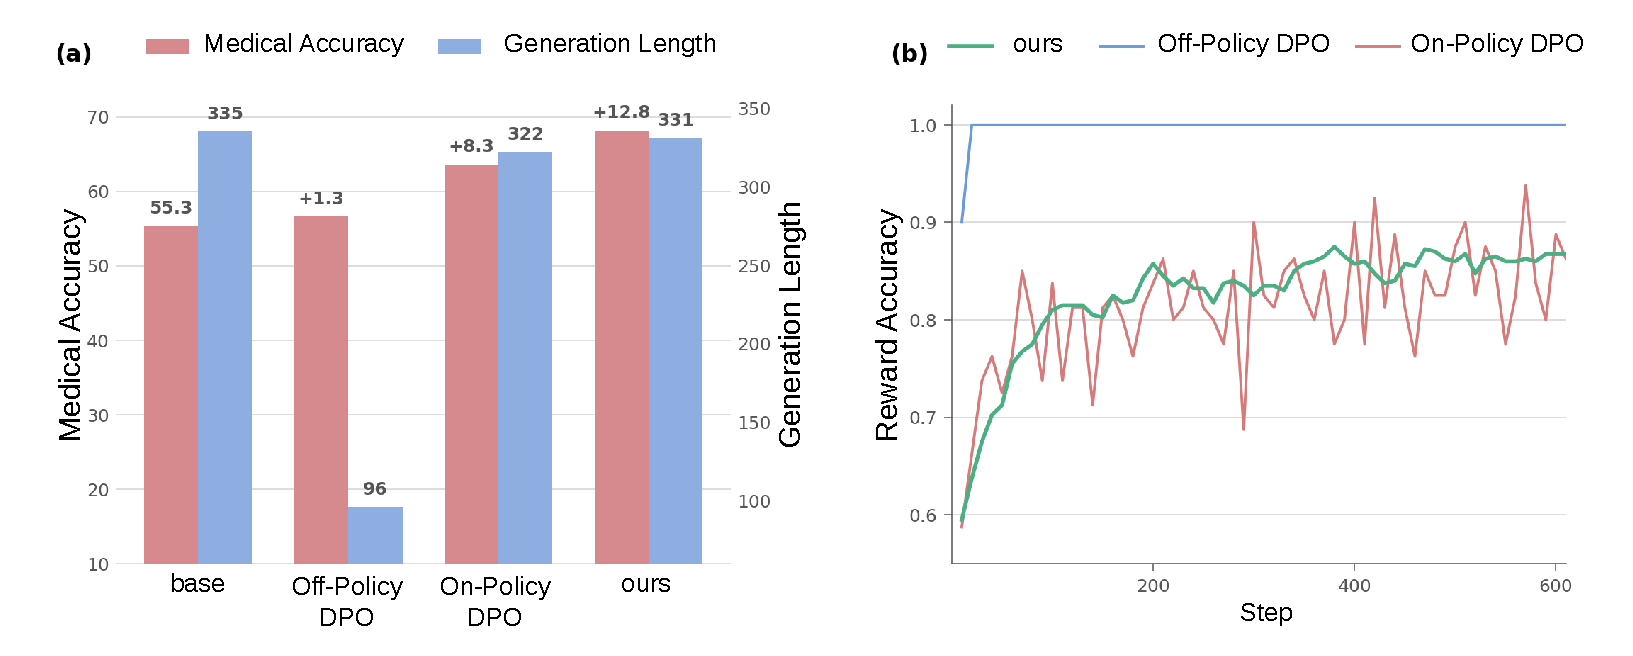
\includegraphics[width=0.85\textwidth]{reward_hacking_plot.pdf}
    \caption{Stylistic shift versus medical accuracy. Using the ground truth as the preferred response causes the model to mimic the length of the rewarded answer instead of improving clinical precision, which shows itself in both the final generation and during training. (a) The medical accuracy of the aligned model compared against its generation length. (b) Reward accuracy measures the fraction of preference pairs for which the implicit DPO reward assigns a higher score to the preferred response than to the rejected response.}
    \label{fig:reward_hacking_analysis}
\end{figure}

In medical DPO, expert preference annotation is often prohibitively expensive, and AI-generated preference labels are unreliable in this domain: large language models used as judges disagree with clinicians in systematic ways~\cite{delucia2026same, rankin2020reliability}. A common alternative is therefore to use the fixed SFT reference response as the preferred answer~\cite{puli2024raddpo, zhu2024mmedpo, liu2025rrg, savage2025fine}.

This construction introduces an off-policy distribution shift~\cite{yang2025mitigating}. Ground-truth medical responses have a characteristic style: they are short, structured, and written in the clipped register of a clinical note. Model responses are typically longer and more explanatory, hedged with qualifications and framed with conversational scaffolding. The two occupy visibly different regions of the space of possible answers. Because DPO optimizes a contrast rather than an absolute notion of correctness, this style gap becomes a second, much stronger signal separating $y^+$ from $y^-$ --- one that is far easier to learn than the clinical distinction. This can confound clinical correctness with response style, a failure mode we refer to as \emph{stylistic reward hacking}.

The issue is particularly acute in clinical alignment because the decisive difference between two responses is often localized to a small span: an anatomical side, a lesion attribute, or an abnormality label. If the preferred and rejected responses also differ in length, syntax, and format, then the clinical difference is one signal among many, and the optimization signal no longer isolates the clinically meaningful error. The model can drive the preference margin arbitrarily high by learning ``be terse and use clinical register'' while leaving its diagnostic behaviour untouched.

Figure~\ref{fig:reward_hacking_analysis} illustrates this effect by comparing model outputs and reward accuracy under \texttt{off-policy} and \texttt{on-policy} preference construction. The diagnostic is the divergence between two curves that ought to move together. Reward accuracy --- the fraction of preference pairs for which the implicit DPO reward correctly ranks $y^+$ above $y^-$ --- measures how well the model has satisfied the training objective. Medical accuracy measures whether it answers clinical questions correctly. Under off-policy DPO, high reward accuracy together with low medical accuracy indicates reward hacking: the model becomes better at satisfying the preference objective without necessarily correcting the clinically relevant visual finding. The generation-length panel identifies the mechanism, showing the aligned model's outputs collapsing toward the length of the ground-truth references. In contrast, on-policy preference construction keeps the response style closer to the model's own outputs, so the two curves track each other.

This suggests a remedy that does not require expert annotation. If the preferred and rejected responses are drawn from the same stylistic distribution --- specifically, if both are the model's own generations and differ only where a clinical span was edited --- then style is held constant by construction and the only remaining signal is the clinical one. This is the principle behind the on-policy preference construction developed in Section~\ref{sec:met:data}, and it is validated empirically in Section~\ref{sec:res:abl-style}.

\subsection{Failure Mode III: The Geometry of the KL Regularizer}
\label{sec:ana:kl}

In clinical alignment, the choice of regularizer $\mathbb{D}_{\text{KL}}$ determines how the updated policy $\pi_\theta$ trades off distributional coverage against precision. Although the standard $\mathcal{L}_{\text{RRPO}}$ utilizes a forward token-wise KL (FKL) to anchor the policy to the base model, the distributional characteristics of the regularizer are critical for high-stakes medical factuality. The two directions are not interchangeable, and neither is sufficient alone.

\subsubsection{Forward KL: Coverage at the Cost of Precision}

The forward term $\mathbb{D}_{\text{KL}}(\pi_{\text{ref}} \parallel \pi_\theta)$ minimizes the divergence by ensuring that $\pi_\theta$ places probability mass wherever the reference $\pi_{\text{ref}}$ does. At the token level $y_t$, the optimization behaves as:
\begin{equation*}
\begin{split}
\arg \min_{\theta} D_{FKL} &= \arg \min_{\theta} D_{KL}(\pi_{\text{ref}} \parallel \pi_\theta) \\
&= \arg \min_{\theta} \mathbb{E}_{y \sim \pi_{\text{ref}}} \left[ \log \frac{\pi_{\text{ref}}(y \mid x)}{\pi_\theta(y \mid x)} \right] \\
&= \arg \max_{\theta} \mathbb{E}_{y \sim \pi_{\text{ref}}} [\log \pi_\theta(y \mid x)].
\end{split}
\end{equation*}

The final line is maximum likelihood estimation of the policy under samples drawn from the reference. Its behaviour follows from the asymmetry of the integrand: the objective is infinite wherever $\pi_{\text{ref}}$ has mass and $\pi_\theta$ does not, but finite --- and bounded --- wherever $\pi_\theta$ has mass and $\pi_{\text{ref}}$ does not. Forward KL therefore punishes the policy for \emph{dropping} modes and is indifferent to the policy \emph{adding} them. This requires $\pi_\theta$ to cover all modes of the reference model. In a medical context, this ensures the model retains the linguistic variety and general clinical knowledge of the base model. However, it can also force the model to preserve low-precision modes --- including exactly those hallucination-prone continuations that alignment was meant to remove.

\subsubsection{Reverse KL: Precision at the Cost of Diversity}

The reverse term $\mathbb{D}_{\text{KL}}(\pi_\theta \parallel \pi_{\text{ref}})$ (RKL) encourages $\pi_\theta$ to concentrate its mass on the high-probability regions of the reference. The objective can be decomposed as:
\begin{equation*}
\begin{split}
\arg \min_{\theta} D_{RKL} &= \arg \min_{\theta} D_{KL}(\pi_\theta \parallel \pi_{\text{ref}}) \\
&= \arg \min_{\theta} \mathbb{E}_{y \sim \pi_\theta} \left[ \log \frac{\pi_\theta(y \mid x)}{\pi_{\text{ref}}(y \mid x)} \right] \\
&= \arg \max_{\theta} \mathbb{E}_{y \sim \pi_\theta} [\log \pi_{\text{ref}}(y \mid x)] + \mathcal{H}(\pi_\theta(y \mid x)).
\end{split}
\end{equation*}

The decomposition, given as Equation~\ref{eq:rkl-decomp} in Section~\ref{sec:bg:kl}, separates two competing pressures. The first term rewards the policy for placing mass where the reference finds it likely; the second, the entropy of the policy, opposes total collapse onto a single mode. The expectation is taken under $\pi_\theta$ rather than $\pi_{\text{ref}}$, which is what makes RKL an \emph{on-policy} regularizer: it evaluates the reference only at points the current policy actually visits. By maximizing the log-probability of the reference under the current policy's samples, it penalizes the model for straying into regions of the token space that the reference model finds unlikely. This tail-suppression is vital for medical LVLMs, as it prevents the model from generating spuriously attractive but clinically incorrect tokens --- the fluent, confident, wrong continuation is precisely a low-reference-probability region that forward KL would leave untouched.

\subsubsection{The Case for a Bidirectional Regularizer}

\begin{figure}[t]
    \centering
    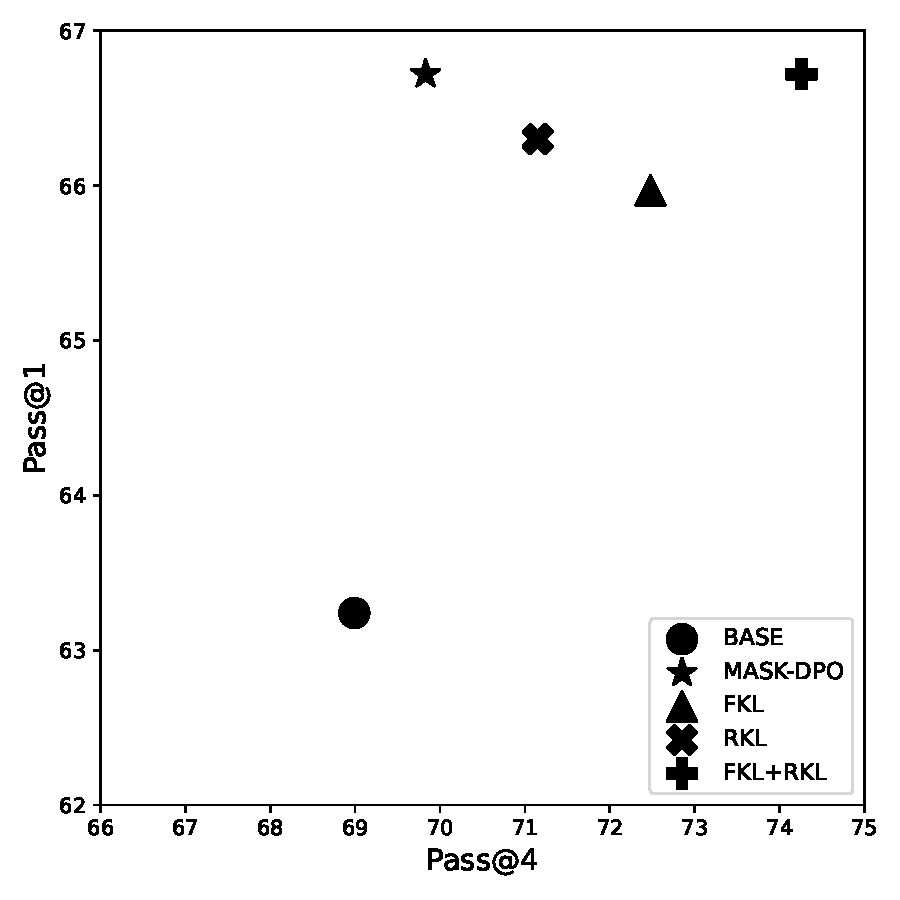
\includegraphics[width=0.55\textwidth]{KL_PLOT.pdf}
    \caption{Comparison of Pass@1 versus Pass@4 across different regularization strategies. The bidirectional KL (FKL+RKL) achieves the highest clinical precision while maintaining the distributional richness required for complex reasoning.}
    \label{fig:tkl_rtkl_comparison}
\end{figure}

Figure~\ref{fig:tkl_rtkl_comparison} analyzes the resulting trade-off between distributional coverage and clinical precision. The two axes are chosen to separate the two effects: Pass@1 measures the precision of the single most likely answer, while Pass@4 measures whether a correct answer appears anywhere among four samples and is therefore sensitive to a collapse in output diversity. A regularizer that improves precision by narrowing the output distribution will raise Pass@1 while flattening or reducing Pass@4.

Samples are drawn with temperature $0.7$ and nucleus sampling at $p = 0.9$; Pass@4 therefore reflects the diversity of the model's output distribution under a standard decoding configuration rather than under an artificially flattened one.

This is what the isolated variants exhibit. While RKL enforces high-precision outputs, its mode-seeking nature often triggers a collapse into repetitive responses. Conversely, FKL acts as a necessary safeguard, anchoring the model to the diverse reasoning traces and linguistic richness of the base policy, at the cost of retaining low-precision modes. The results suggest that optimization under either force in isolation is insufficient for high-stakes medical alignment. A balanced regularization ensures the policy achieves rigorous clinical accuracy without sacrificing the interpretive variety that is essential for complex medical reasoning.

\subsection{Failure Mode IV: The Absence of Grounding Constraints}
\label{sec:ana:grounding}

The three failure modes above all concern the textual side of the objective. A fourth is orthogonal to them: none of Equations~\ref{eq:dpo} or~\ref{eq:rrpo} contains any term that ties a clinical assertion to the image evidence supporting it.

This matters because a vision-language model has two routes to a correct answer. It can read the image, or it can exploit a linguistic prior --- base rates over findings, correlations between question phrasing and answer, or the anatomical defaults of the modality. Both routes produce the same token sequence, and a purely textual preference objective rewards both identically. A model that answers ``left lung'' because the lesion is visibly on the left and a model that answers ``left lung'' because that answer is more common in the training distribution are indistinguishable to Equation~\ref{eq:dpo}. Alignment on such an objective can therefore increase measured accuracy while leaving --- or even worsening --- the model's actual dependence on visual evidence.

Figure~\ref{fig:framework_overview} shows this directly. The DPO-aligned model produces the correct answer, but its visual attention remains as diffuse as the unaligned base model's; the correction was learned as a textual association, not as a grounding improvement. The layer-wise measurements in Section~\ref{sec:res:grounding} confirm the pattern quantitatively across both backbones.

Existing multimodal preference methods do introduce image-side signal, but typically through coarse global perturbations --- cropping, whole-image noise, or blacking out the image entirely. These are too blunt for the clinical case. Removing the entire image tests whether the model uses vision at all, which is a much weaker property than whether it uses the \emph{diagnostically decisive region}. A model can retain a globally sensible reading of a chest radiograph while being completely insensitive to the small focal opacity that determines the answer. Isolating that sensitivity requires perturbing the lesion specifically while leaving the rest of the anatomy intact, and the ablation in Section~\ref{sec:res:abl-visual} quantifies how much this distinction is worth.

\subsection{Why the Four Failures Compound}
\label{sec:ana:compound}

The four failure modes have been presented separately, but the central claim of this thesis is that in a clinical setting they interact, and that this interaction explains why addressing any one in isolation yields the inconsistent gains reported in the literature~\cite{kim2026benchmarking}.

Three couplings matter.

\textbf{Coarse rewards and stylistic confounds reinforce each other.} A fine-grained reward is a mechanism for concentrating the training signal on the tokens that carry the clinical distinction. That mechanism is worthless if a stylistic feature separates the preference pair more reliably than the clinical content does, because the model will exploit the easier feature first, and the gradient will vanish before the harder distinction is ever engaged. Conversely, style-matched pairs deliver much less benefit under a sequence-level reward, since the informative difference is then a small fraction of a signal that is spread uniformly across the response. The two remedies are close to useless apart and complementary together.

\textbf{Localizing the reward destabilizes the policy unless the regularizer is restored.} As Section~\ref{sec:bg:alignment} showed, DPO's KL constraint lives entirely inside the implicit reward's $\pi_{\text{ref}}$ denominator. Restricting the ranking loss to selected positions therefore removes the constraint everywhere else, leaving the policy free to drift on the majority of the response --- the very positions the fine-grained reward has decided not to supervise. This is not a hypothetical: Section~\ref{sec:res:abl-kl} shows a $22$-point collapse on report generation in exactly this configuration. Fine-grained rewards and an explicit regularizer are not two independent improvements but two halves of one change.

\textbf{Neither textual remedy touches grounding.} Both of the couplings above concern which tokens the objective supervises and how the pairs are built. Neither says anything about whether the model consulted the image. A method could fix both and still produce a model that has merely learned better linguistic associations, which is what the DPO grounding curves in Section~\ref{sec:res:grounding} appear to show. Grounding is orthogonal to the textual failures, which is precisely why it needs a separate term rather than better textual supervision.

The practical implication is that an ablation table, which by construction removes one component at a time, systematically understates the value of the combination. Section~\ref{sec:res:abl-visual} finds that removing the visual term costs only $0.38$ points on average --- but that measurement is taken with the fine-grained reward, the style-matched pairs, and the regularizer all still in place. The relevant comparison for the thesis as a whole is not any single ablation but the gap between the full method and standard DPO, which is $5.25$ points on HuatuoGPT.

\subsection{Design Desiderata}
\label{sec:ana:desiderata}

The four analyses above translate into four requirements on an alignment objective for medical LVLMs. Chapter~\ref{section:method} addresses each in turn.

\begin{itemize}
    \item \textbf{D1. Localized reward assignment.} The training signal must be concentrated on the clinically decisive spans that distinguish $y^+$ from $y^-$, rather than distributed uniformly over the response. \emph{Addressed by the fine-grained ranking loss, Section~\ref{sec:met:ranking}.}

    \item \textbf{D2. Style-invariant preference pairs.} The preferred and rejected responses must be drawn from the same stylistic distribution, so that the only systematic difference between them is clinical. \emph{Addressed by on-policy minimal-edit construction, Section~\ref{sec:met:data}.}

    \item \textbf{D3. Bidirectional regularization.} The regularizer must simultaneously suppress low-probability incorrect tails and preserve the base model's coverage, which neither KL direction achieves alone. \emph{Addressed by the bidirectional token-wise KL, Section~\ref{sec:met:kl}.}

    \item \textbf{D4. Explicit evidence grounding.} The objective must contain a term that penalizes confident answers produced without the supporting visual evidence, at the granularity of the lesion rather than the whole image. \emph{Addressed by the dual-constraint ranking loss over lesion-corrupted images, Sections~\ref{sec:met:corruption} and~\ref{sec:met:ranking}.}
\end{itemize}

\section{\ourloss{}: Fine-grained Regularized Medical Preference Optimization}
\label{section:method}

\subsection{Overview}
\label{sec:met:overview}

This chapter develops \ourloss{}, an alignment framework built directly against the four desiderata of Section~\ref{sec:ana:desiderata}. It comprises two halves that are trained jointly: a data construction procedure that produces preference pairs in which style is held constant and the clinically divergent spans are explicitly marked (D1, D2), and a training objective that combines a dual-constraint fine-grained ranking loss over clean and lesion-corrupted images (D1, D4) with a bidirectional token-wise KL regularizer (D3).

Before developing the components, it is worth stating precisely how \ourloss{} departs from RRPO, its closest antecedent. Three of RRPO's design choices do not survive the move to a clinical setting.

First, RRPO relies on a forward KL divergence term as its regularizer. This tends to preserve the coverage and diversity of $\pi_{\text{ref}}$, yet it often fails to facilitate the learning of new concepts that lie beyond the distribution of the reference model --- which is exactly what domain adaptation to medicine requires.

Second, RRPO imposes an overly rigid constraint by requiring the rejected response to strictly mirror a ground-truth template, which necessitates perfectly paired correct and incorrect phrases. In practical settings, such a constraint is often unrealistic, as a single phrase in the preferred response may correspond to multiple segments within the rejected response. Consequently, this forceful alignment can cause the model to shift its behaviour too abruptly when encountering new tasks. Rather than achieving seamless adaptation, this approach frequently leads to the forgetting of useful prior knowledge in favour of satisfying an off-policy alignment.

Third, the framework lacks explicit constraints regarding evidence grounding within the visual domain, a factor that is particularly critical for effective alignment in high-stakes environments such as the medical domain.

\subsection{On-Policy Fine-grained Preference Construction}
\label{sec:met:data}

The construction procedure takes an existing medical SFT dataset --- image $v$, question $q$, ground-truth answer $a$ --- and produces preference records in which $y^+$ and $y^-$ are stylistically matched and their clinically divergent spans are delimited by explicit \texttt{<mask>} markers. Figure~\ref{fig:pipeline_overview} gives the overall flow.

\begin{figure}[t]
    \centering
    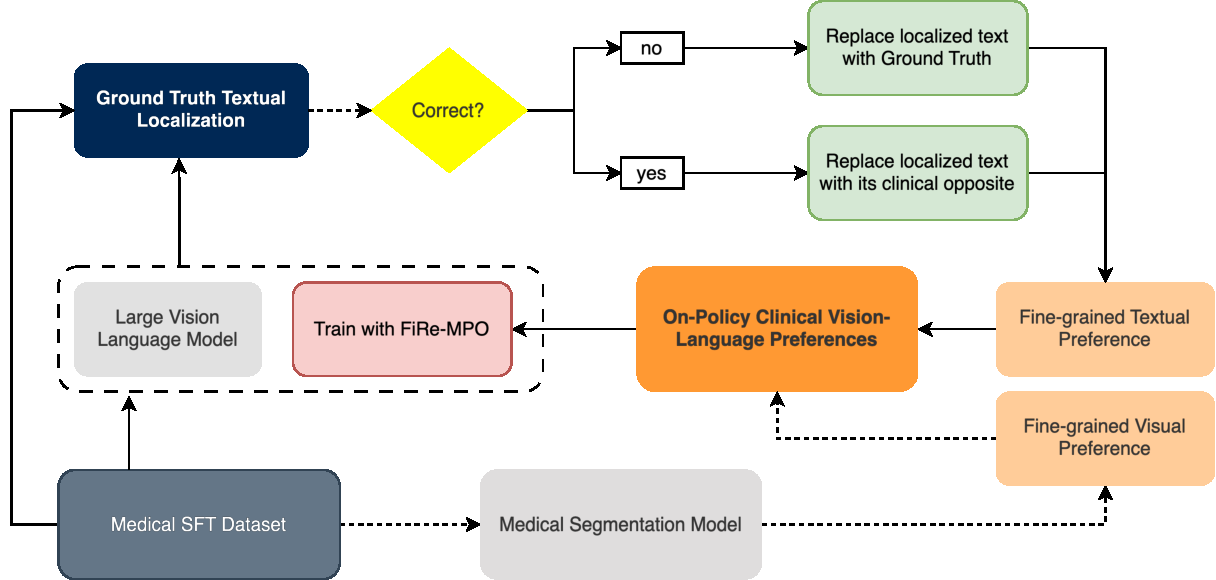
\includegraphics[width=0.85\textwidth]{pipeline.pdf}
    \caption{An overview of the fine-grained on-policy visual-textual preference creation process.}
    \label{fig:pipeline_overview}
\end{figure}

\subsubsection{Sampling On-Policy Responses}

The procedure begins by obtaining a response from $\pi_\theta$ itself for the given $\{v, q\}$, using greedy decoding. This single decision is what makes the construction on-policy, and it is what distinguishes \ourloss{} from the reference-substitution approach analyzed in Section~\ref{sec:ana:reward-hacking}: both members of every resulting preference pair originate from the model's own output distribution, so the stylistic confound is eliminated by construction rather than corrected for after the fact.

Greedy decoding is chosen over sampling for a specific reason. The purpose of the sampled response is to expose the model's \emph{characteristic} behaviour --- what it will actually produce at inference time --- so that the correction targets an error the model genuinely makes. A high-temperature sample would exhibit errors drawn from the tail of the distribution, which the model would rarely commit in practice, and correcting those spends the training signal on failures that do not matter. The trade-off is coverage: greedy decoding yields one response per input, so the corpus is exactly as large as the underlying SFT dataset and no larger, whereas sampling could generate several pairs per input.

Because the response is the model's own, the corpus is specific to the backbone that generated it. Aligning a different model requires regenerating the textual side of the corpus. Section~\ref{sec:exp:corpus} quantifies the consequence: the two backbones yield corpora that differ in size and, more interestingly, in composition, since they make errors on different fractions of the data.

\subsubsection{Stage One: Localizing the Clinical Claim}

The sampled response is passed to a language model (\texttt{GPT-4o-mini}) together with the question and the ground-truth answer. The prompt, reproduced in full as Figure~\ref{fig:prompt_stage1} in Appendix~\ref{app:prompts}, asks for a single JSON object containing four fields:

\begin{itemize}
    \item \texttt{answer\_sentence} --- the minimal phrase or clause from the model's answer that states the final answer, in the model's exact wording.
    \item \texttt{final\_answer} --- the conclusive answer extracted in as few words as possible.
    \item \texttt{is\_correct} --- whether that answer is correct given the ground truth.
    \item \texttt{opposite\_answer} --- the answer sentence modified as little as possible into a medically plausible alternative.
\end{itemize}

The design of these fields is what enforces minimal editing. By requiring the extractor to quote the model's exact wording and to produce the counterfactual by modifying that quotation as little as possible, the resulting edit is confined to the clinical span; the surrounding sentence is carried over verbatim.

The \texttt{is\_correct} field then determines which branch of the construction applies:

\begin{itemize}
    \item If the output contains clinically designated errors, we substitute only the erroneous medical statements with ground-truth information to form $y^+$, while the original output serves as $y^-$.
    \item Conversely, if the initial response is already correct, we use it as $y^+$ and generate $y^-$ by altering the response with plausible medical counterfactuals --- the \texttt{opposite\_answer} field.
\end{itemize}

In both scenarios, the model's original linguistic style is preserved to allow on-policy alignment. The second branch matters more than it might appear: it means that questions the model already answers correctly still contribute a training signal, in the form of an explicit contrast against a plausible-but-wrong alternative, rather than being discarded.

\subsubsection{Stage Two: Localizing the Divergent Spans}

Given $y^+$ and $y^-$, a second call identifies exactly which phrases differ. The prompt presents the two sentences and asks the model to wrap only the differing phrases in \texttt{<mask>} and \texttt{</mask>} tags, with the instruction that the marked phrases be as short as possible.

These tags are the mechanism by which desideratum D1 is realized. They are added to the tokenizer as special tokens, and at training time the trainer converts them into a binary phrase mask over token positions --- every position strictly between a \texttt{<mask>} and its matching \texttt{</mask>} is marked, and the tag tokens themselves are then stripped from the input so the model never sees them. The ranking loss and the KL regularizer are both restricted to the marked positions. A single response may contain several such spans; the mask construction handles multiple pairs in one sequence.

\subsubsection{Adapting the Pipeline to Report Generation}

Radiology report generation does not fit the question-answer template, because there is no single answer span to localize --- a report contains many independent clinical assertions. The pipeline is therefore restructured for IU-Xray, using \texttt{Gemini 3 Flash Preview} in place of \texttt{GPT-4o-mini}.

Stage one becomes a constrained rewrite. The model's generated report (Report A) and the ground-truth report (Report B) are presented together, and the model is asked to use the facts in Report B to replace a few medical words in Report A. The prompt imposes three constraints that together preserve style while forcing a clinical change: \emph{structural locking} (the format of Report A must be preserved), \emph{token parsimony} (at most two or three words per sentence may be changed), and \emph{clinical significance} (synonym substitutions such as ``clear'' for ``normal'' are explicitly rejected). If every fact in Report B is already present in Report A, the model instead introduces a clinical error to create the rejected member of the pair. Stage two is then the same masked-difference step as in the VQA pipeline, applied to the two reports. Both report-side prompts are given as Figure~\ref{fig:prompt_stage2}.

\subsection{Lesion-Targeted Visual Corruption}
\label{sec:met:corruption}

The visual half of the construction produces, for each record, a corrupted counterpart $v'$ of the image. Section~\ref{sec:ana:grounding} argued that global perturbations are too blunt for the clinical case: what must be tested is not whether the model uses the image at all, but whether it uses the diagnostically decisive region. The corruption is therefore targeted at that region and leaves the surrounding anatomy intact.

The procedure has three steps. First, a short text prompt naming the clinical concept relevant to the query is extracted from each record by a language model --- for instance, the finding or anatomical structure that the question asks about. Second, this prompt is passed to MedSAM3-v1~\cite{liu2025medsam3}, a purely text-guided medical segmentation model, which returns segmentation masks for the named concept; where the model returns several detections, their union is taken as a single region. Third, zero-mean Gaussian noise is added per channel \emph{inside the mask only}, at a standard deviation of $45$ on the $0$--$255$ intensity scale, and the result is clipped back to the valid range.

Three properties of this choice of corruption are deliberate.

\emph{It destroys evidence without announcing itself.} Additive noise inside an anatomically plausible boundary leaves an image that still reads as a radiograph or CT slice. Cropping or blacking out a region produces an image that is trivially identifiable as degraded, which gives the model an alternative route to satisfying the objective: it can learn to detect the corruption and condition on that, rather than learning to depend on the lesion. Section~\ref{sec:res:abl-visual} shows both of those coarser strategies performing markedly worse, which is consistent with this concern.

\emph{It is local.} Everything outside the mask is bit-identical to the clean image. The paired comparison therefore isolates the contribution of the query-relevant region specifically, rather than the contribution of the image as a whole. This is the property that distinguishes the objective from the global perturbations used in prior multimodal preference work, as discussed in Section~\ref{sec:rel:multimodal}.

\emph{It is calibrated to remove the finding rather than the anatomy.} A standard deviation of $45$ on a $0$--$255$ scale is large enough to obliterate the texture differences that distinguish pathological from healthy tissue, but leaves gross structure discernible. The intent is to make the specific diagnostic claim unsupportable while keeping the image interpretable enough that a well-grounded model would produce a hedged rather than a nonsensical response.

Two fallbacks handle the cases where the pipeline cannot deliver a localized region. If no concept prompt could be extracted for a record, noise is applied to the whole image instead. If a prompt exists but MedSAM3 returns no mask, a lighter global perturbation ($\sigma = 12$) is applied. Each record carries a note recording which path was taken, so that fallback cases can be identified during analysis, and a flag indicating whether a usable corrupted image is available at all --- records without one simply do not contribute to the visual term of the loss. Section~\ref{sec:exp:corpus} reports how often each path is taken, and the figure is high enough to qualify the results: on SLAKE only $64.0\%$ of records receive genuinely lesion-targeted corruption.

Report generation is handled differently by design. A report-generation prompt asks for a description of the whole study rather than about one localized finding, so there is no single query-relevant region to segment, and holistic image-level noise is used throughout. The visual term therefore tests dependence on the image as a whole in that setting rather than on a specific finding, which is a weaker property than the one tested on the VQA datasets.

Section~\ref{sec:res:abl-visual} compares this lesion-targeted strategy against cropping, image-level noise, and full masking, and finds the localized variant substantially stronger on all three benchmarks.

\subsection{The Dual-Constraint Ranking Loss}
\label{sec:met:ranking}

Given the subtle visual nuances in the medical domain, our objective is to prevent the model from hallucinating correct-sounding responses when essential visual evidence is absent or corrupted. We achieve this by structuring the ranking loss around a dual constraint.

First, we define preference pairs $(q, v, y^+) \succ (q, v, y^-)$, which align $\pi_\theta$ toward medically accurate answers when supported by valid visual evidence $v$.

Second, we introduce pairs $(q, v', y^-) \succ (q, v', y^+)$, which compel the model to refrain from providing a definitive response when the underlying visual evidence is corrupted ($v'$). This ensures that the model prioritizes visual evidence over linguistic priors, effectively penalizing correct guesses made for the wrong reasons.

The reversal in the second pair is the crux of the design and deserves emphasis, because it is counterintuitive: the objective explicitly prefers the \emph{clinically wrong} answer under the corrupted image. It does so because the quantity being supervised is not correctness but \emph{warrant}. When the evidence supporting a specific claim has been destroyed, a model that still asserts that claim with undiminished confidence is demonstrating that the claim was never grounded in the image to begin with. Preferring $y^+$ under both $v$ and $v'$ would reward exactly that behaviour. Requiring the preference to \emph{flip} when the evidence is removed forces the model's confidence in the clinical span to be a function of the visual evidence rather than of a linguistic prior. Section~\ref{sec:res:abl-visual} tests this against the two natural alternatives --- preferring $(v, y^+)$ over $(v', y^+)$, and over $(v', y^-)$ --- and finds both weaker.

Note that in both cases, we provide a fine-grained reward only on the clinically divergent tokens between $y^+$ and $y^-$, that is, on the positions selected by the phrase mask of Section~\ref{sec:met:data}. The ranking loss is defined as:
\begin{equation}\label{eq:firempo-rank}
\begin{split}
\mathcal{L}^{\text{(Rank)}}_{\text{FiRe-MPO}}(\pi_{\theta};\pi_{\text{ref}}) = &
-\mathbb{E}
\biggl[
\log \sigma \left(\sum_{i} r_\theta(v,q,y^+_i) - \sum_{i} r_\theta(v,q,y^-_i)\right) \\
& + \gamma\log \sigma \left(\sum_{i} r_\theta(v',q,y^-_i) - \sum_{i} r_\theta(v',q,y^+_i)\right)
\biggr],
\end{split}
\end{equation}
where the index $i$ ranges over masked positions only and $\gamma$ weights the grounding term relative to the primary preference. Setting $\gamma = 0$ recovers a purely textual fine-grained objective, which is the \emph{w/o visual pref.} ablation of Section~\ref{sec:res:abl-visual}.

\subsection{The Bidirectional Token-wise KL Regularizer}
\label{sec:met:kl}

Our goal is to enable the policy model to preserve the rich, generalized prior knowledge of the base model while simultaneously allowing it to assimilate new, specialized domain knowledge that may lie outside the base model's original distribution.

As established in Section~\ref{sec:ana:kl}, the forward KL divergence $\mathbb{D}_{\text{KL}}(\pi_{\text{ref}} \parallel \pi_\theta)$, as employed in RRPO, is mean-seeking, forcing the policy model to maintain the broad coverage of the reference distribution. Although this successfully preserves the base model's diverse vision-language capabilities, it is overly restrictive: it heavily penalizes the policy for shifting its probability mass to learn the new concepts necessary for adapting to specific fields such as medicine. Conversely, the reverse KL divergence $\mathbb{D}_{\text{KL}}(\pi_\theta \parallel \pi_{\text{ref}})$ is inherently mode-seeking, allowing the model to learn new concepts through effective tail suppression. However, it often induces a severe lack of generation diversity.

To address these limitations, we replace the unidirectional constraint with a bidirectional, token-wise KL regularizer. This balances coverage preservation against tail suppression by simultaneously applying both forward and reverse KL constraints at the token level:
\begin{equation}\label{eq:firempo-kl}
\begin{split}
\mathcal{L}^{\text{(KL)}}_{\text{FiRe-MPO}}(\pi_\theta; \pi_{\text{ref}}) = &
- \mathbb{E} \biggl[ \sum_t \Big( \lambda \mathbb{D}_{\text{KL}} \big(\pi_{\text{ref}}(y_t \mid v,q,y_{<t}) \parallel \pi_\theta(y_t \mid v,q,y_{<t}) \big) \\
& + (1-\lambda) \mathbb{D}_{\text{KL}} \big(\pi_\theta(y_t \mid v,q,y_{<t}) \parallel \pi_{\text{ref}}(y_t \mid v,q,y_{<t}) \big) \Big) \biggr],
\end{split}
\end{equation}
where $\lambda$ is a hyperparameter that dictates the relative influence of each constraint. The endpoints recover the unidirectional cases: $\lambda = 1$ gives the forward-only regularizer of RRPO, and $\lambda = 0$ gives a purely reverse-KL objective. Both are ablated in Section~\ref{sec:res:abl-kl}, alongside removing the regularizer entirely.

The two terms are not redundant, and it is worth being precise about why a single coefficient can balance them. Because the divergences are evaluated between the same pair of distributions at the same token positions, they differ only in which distribution supplies the expectation. The forward term is dominated by positions where the reference is confident and the policy has moved away, and penalizes the policy for abandoning reference-supported continuations. The reverse term is dominated by positions where the policy has become confident in something the reference finds unlikely, and penalizes exactly the fluent-but-unsupported continuation that Section~\ref{sec:bg:kl} identifies as the characteristic medical failure. A given update can incur one penalty without the other, so the sum is not merely a rescaling of either term; $\lambda$ selects which kind of deviation the optimizer is more willing to tolerate.

Like the ranking loss, this sum is restricted to the masked phrase positions rather than applied over the full response. This is a deliberate pairing rather than an implementation convenience. The ranking term concentrates the preference signal on the clinical spans, which is precisely where the policy is being pushed hardest and therefore where uncontrolled drift is most likely; constraining the same positions places the regularizer where the pressure is. It also keeps the two terms commensurable, since both are sums over the same index set, which is what makes a single coefficient $\alpha$ meaningful in Equation~\ref{eq:firempo-total}.

\subsection{The Complete Objective}
\label{sec:met:objective}

The complete \ourloss{} objective unifies the ranking loss with the KL regularizer:
\begin{equation}\label{eq:firempo-total}
\mathcal{L}_{\text{FiRe-MPO}}(\pi_\theta; \pi_{\text{ref}}) = \mathcal{L}^{\text{(Rank)}}_{\text{FiRe-MPO}}(\pi_{\theta};\pi_{\text{ref}}) + \alpha \cdot \mathcal{L}_{\text{FiRe-MPO}}^{\text{(KL)}}(\pi_\theta; \pi_{\text{ref}}),
\end{equation}
where $\alpha$ is a loss coefficient controlling the relative influence of the fine-grained reward and the model divergence.

The objective therefore has four hyperparameters. $\beta$ is the standard DPO preference temperature inside $r_\theta$; $\gamma$ weights the visual grounding term; $\lambda$ sets the balance between the two KL directions; and $\alpha$ scales the regularizer against the ranking loss. Default values are $\beta = 0.1$, $\gamma = 0.1$, $\lambda = 0.5$, and $\alpha = 0.01$, with the full configuration given in Appendix~\ref{app:impl}. Appendix~\ref{app:pseudocode} gives the objective in executable form.

\subsection{Implementation}
\label{sec:met:implementation}

\subsubsection{Phrase Masking and Batch Construction}

The \texttt{<mask>} and \texttt{</mask>} delimiters are registered as special tokens on the tokenizer before training. During collation, each sequence is scanned for delimiter pairs and a binary mask is produced marking every position strictly between a \texttt{<mask>} and its matching \texttt{</mask>}; the delimiter tokens themselves are then removed from the input, together with their positions in the mask, so that the model is never conditioned on markup that will not appear at inference time. Sequences containing an unmatched \texttt{<mask>} are rejected rather than silently truncated.

Because the ranking loss in Equation~\ref{eq:firempo-rank} contains two preference terms over two different images, each training step requires forward passes over four sequence variants --- $(v, y^+)$, $(v, y^-)$, $(v', y^+)$, $(v', y^-)$ --- under both the policy and the frozen reference. The collator carries the corrupted image alongside the clean one, together with a per-example boolean indicating whether a corrupted image exists for that record; the visual term is masked out for examples where it does not, so that records whose lesion could not be segmented still contribute their textual preference.

\subsubsection{Parameter-Efficient Adaptation}

Following standard preference learning protocols, we use Low-Rank Adaptation (LoRA)~\cite{hu2022lora}. LoRA is applied exclusively to the LLM component of the LVLM, while the vision encoder and cross-modal projectors remain frozen to preserve the fundamental perceptual features learned during pre-training. This choice interacts with the grounding objective in a way worth making explicit: because the vision tower is frozen, the visual preference term cannot improve grounding by changing how the image is encoded. It can only change how the language model \emph{attends to and uses} the existing visual representation. The grounding improvements reported in Section~\ref{sec:res:grounding} are therefore attributable to the objective rather than to visual representation learning.

A practical benefit of LoRA in this setting is that the reference model does not need to be held separately in memory: reference log-probabilities are obtained by disabling the adapters on the same base weights.

\subsubsection{Computational Cost}

The dominant cost relative to standard DPO is the number of forward passes per optimization step. DPO requires two policy and two reference passes, over $(v, y^+)$ and $(v, y^-)$. \ourloss{} requires four of each, because of the additional pair over $v'$. The KL regularizer adds no forward passes --- it is computed from logits already materialized by the $(v, y^+)$ pass --- but it does require retaining full vocabulary-sized logits for both policy and reference at those positions in order to evaluate the divergence, which is the dominant memory term. Backward cost is unchanged in structure, since only the LoRA parameters receive gradients.

Table~\ref{tab:cost} reports the measured cost of a \ourloss{} training step on \texttt{Qwen3-VL-4B-Instruct} over the SLAKE corpus, on a single H200 with 143\,GB of memory. Two practical observations follow from these measurements.

\begin{table}[ht]
\centering
\small
\caption{Measured training cost of \ourloss{} on \texttt{Qwen3-VL-4B-Instruct} over the SLAKE preference corpus, at the batch size and LoRA configuration of Appendix~\ref{app:impl}. Steady-state step time excludes the first optimization step, which is roughly an order of magnitude slower due to kernel autotuning and allocator warmup.}
\label{tab:cost}
\begin{tabular}{lr}
\toprule
\textbf{Quantity} & \textbf{Measured} \\
\midrule
Forward passes per step (policy + reference) & $4 + 4$ \\
Steady-state step time & 4.3--4.6\,s \\
First-step time (warmup) & $\approx$74\,s \\
Steps per epoch (SLAKE, global batch 8) & 610 \\
Wall-clock per epoch & $\approx$44\,min \\
Peak GPU memory (gradient checkpointing on) & $\approx$139\,GB \\
Peak GPU memory (gradient checkpointing off) & exceeds 143\,GB \\
\bottomrule
\end{tabular}
\end{table}

First, gradient checkpointing is not optional at this configuration. Disabling it --- ordinarily an attractive trade on a large-memory device, since it removes the recomputation of activations during the backward pass --- exhausts the 143\,GB card. The reason is the combination of eight forward passes over sequences that each carry on the order of a thousand visual tokens, together with the vocabulary-sized logits the KL term requires. The peak of roughly 139\,GB with checkpointing enabled also means that two training runs cannot share one device, which constrains how a large sweep must be scheduled.

Second, the cost is dominated by the visual pair rather than by the regularizer. The extra $(v', y^{\pm})$ passes double the forward work relative to DPO, whereas the bidirectional KL term reuses logits that have already been computed. A practitioner constrained on compute should therefore reduce $\gamma$ or drop the visual term before touching $\alpha$; Section~\ref{sec:res:abl-kl} shows the regularizer to be the component whose removal is most damaging, and Section~\ref{sec:res:dynamics} shows it to be the cheapest.

The data construction pipeline additionally incurs a one-off cost, paid once per dataset rather than per training step: two language model calls per record for the textual pipeline, and one segmentation pass plus one prompt-extraction call per record for the visual pipeline. For SLAKE this amounts to roughly ten thousand language model calls and five thousand segmentation passes, after which the corpus is fixed and reusable across every subsequent training run.

\section{Experimental Setup}
\label{section:setup}

\subsection{Base Models}
\label{sec:exp:models}

We evaluate \ourloss{} using two state-of-the-art open-source backbones, chosen so that the two ends of the medical-specialization spectrum are both represented.

\texttt{HuatuoGPT-Vision-7B}~\cite{chen2024towards} is a specialized medical LVLM pre-trained on extensive medical image-text pairs, making it a strong domain-specialized backbone for clinical vision-language alignment. Because it has already absorbed a large amount of medical visual knowledge, it tests whether fine-grained alignment still adds value on top of domain pretraining.

\texttt{Qwen3-VL-4B-Instruct}~\cite{bai2025qwen3} is a highly efficient multimodal model that utilizes a sophisticated visual-language adapter for high-resolution image perception, providing a robust baseline for assessing both medical-specific and general-purpose multimodal alignment capabilities. It has had no medical pretraining, so it tests whether the method can install clinical behaviour rather than merely refine it.

The pair is also informative because they differ in scale ($7$B versus $4$B), so consistent gains across both are evidence that the method is not exploiting a property of one particular model.

\subsection{Datasets}
\label{sec:exp:datasets}

We utilize three benchmark datasets that span diverse clinical modalities and tasks.

\textbf{VQA-RAD}~\cite{lau2018dataset} is a manually constructed dataset containing $315$ radiology images of the head, chest, and abdomen, paired with $3{,}515$ professional-grade question-answer pairs. We utilize the full dataset, encompassing both open-ended and binary ``yes/no'' queries. It is the smallest of the three and the most clinically authoritative, since every question was written by a physician.

\textbf{SLAKE}~\cite{liu2021slake} is a semantically-labelled bilingual dataset featuring $642$ images and over $14{,}000$ QA pairs. For our experiments, we utilize only the English portion of the dataset and focus on the visual-textual pairs, without incorporating the semantic labels or the medical knowledge graph. This restriction is deliberate: the knowledge graph would supply structured clinical information that our pipeline is meant to derive from the image and the ground-truth answer alone.

\textbf{IU-Xray}~\cite{demner2016preparing} comprises $7{,}470$ dual-view chest X-ray images and $3{,}955$ corresponding reports, and is used for clinical report generation. It exercises a different regime from the two VQA datasets: outputs are long-form and contain many independent clinical assertions, which is precisely the setting in which sequence-level rewards are weakest.

Table~\ref{tab:splits} records the split sizes actually used. All evaluation is conducted on the standard in-distribution test split of each dataset.

\begin{table}[ht]
\centering
\small
\caption{Dataset splits used for training and evaluation. SLAKE counts are for the English subset only. VGMED is evaluation-only.}
\label{tab:splits}
\begin{tabular}{lrrrl}
\toprule
\textbf{Dataset} & \textbf{Train} & \textbf{Val} & \textbf{Test} & \textbf{Task} \\
\midrule
SLAKE (English)  & 4{,}919 & 1{,}053 & 1{,}061 & VQA (416 closed / 645 open) \\
VQA-RAD          & 1{,}793 & --      & 451     & VQA (closed and open) \\
IU-Xray          & 2{,}069 & 296     & 590     & Report generation \\
\midrule
VGMED (loc)      & --      & --      & 1{,}388 & Grounding \\
VGMED (att)      & --      & --      & 1{,}388 & Grounding \\
\bottomrule
\end{tabular}
\end{table}

\subsection{Preference Corpus Statistics}
\label{sec:exp:corpus}

Because the preference corpus is generated per backbone --- the responses are sampled from the model being aligned --- each backbone has its own dataset, and the two differ in size and composition. Table~\ref{tab:corpus} reports the resulting corpora, which are not characterized in the original paper.

\begin{table}[ht]
\centering
\small
\caption{On-policy preference corpora produced by the pipeline of Section~\ref{sec:met:data}, one per backbone and dataset. \emph{Pairs} is the number of preference records; \emph{With $v'$} is the number that carry a corrupted image and therefore contribute to the visual term; \emph{Already correct} is the share of records where the model's own sampled response was clinically correct, so the rejected member was generated as a counterfactual rather than the preferred member being repaired.}
\label{tab:corpus}
\begin{tabular}{llrrr}
\toprule
\textbf{Backbone} & \textbf{Dataset} & \textbf{Pairs} & \textbf{With $v'$} & \textbf{Already correct} \\
\midrule
\multirow{3}{*}{HuatuoGPT-Vision-7B}
 & SLAKE   & 4{,}888 & 4{,}888 & 57.4\% \\
 & VQA-RAD & 1{,}786 & 1{,}786 & 59.7\% \\
 & IU-Xray & 2{,}015 & 1{,}996 & 29.1\% \\
\midrule
\multirow{3}{*}{Qwen3-VL-4B-Instruct}
 & SLAKE   & 4{,}902 & 4{,}877 & 63.4\% \\
 & VQA-RAD & 1{,}792 & 1{,}785 & 55.4\% \\
 & IU-Xray & 2{,}026 & 1{,}954 & 26.8\% \\
\bottomrule
\end{tabular}
\end{table}

Two observations follow from this table. First, the corpora are close in size to the underlying training splits, confirming that the pipeline retains nearly every source example rather than discarding the ones it cannot process; the small shortfall in the \emph{With $v'$} column corresponds to records for which no corrupted image could be produced, and those records still contribute their textual preference through the first term of Equation~\ref{eq:firempo-rank}.

Second, the \emph{Already correct} column shows that the two branches of the construction are both heavily used, and in a task-dependent way. On the VQA datasets the models were already correct on roughly $55$--$63\%$ of examples, so the majority of pairs are formed by generating a plausible counterfactual as $y^-$. On report generation the figure drops to under $30\%$, reflecting that a long report is far less likely to be entirely free of clinical error than a short answer. Without the counterfactual branch described in Section~\ref{sec:met:data}, roughly $60\%$ of the VQA training signal would simply not exist.

The corrupted images themselves are \emph{model-agnostic}: corruption depends only on the image and the clinical concept named by the query, not on which policy generated the response. Each dataset's corrupted image set is therefore constructed once and reused across both backbones, which is why the two rows of Table~\ref{tab:corpus} for a given dataset draw on the same pool of $v'$ images.

Table~\ref{tab:corruption_paths} records which corruption path each dataset took. Two of the three are handled by the lesion-targeted procedure of Section~\ref{sec:met:corruption}, with fallbacks where no concept prompt could be extracted or MedSAM3 returned no detection. Report generation is different by design: an IU-Xray prompt asks for a description of the whole study rather than about one localized finding, so there is no single query-relevant region to segment, and holistic image-level noise is used throughout.

\begin{table}[ht]
\centering
\small
\caption{Corruption path by dataset. Corruption is model-agnostic, so these counts apply to both backbones. \emph{Lesion-targeted} is the procedure of Section~\ref{sec:met:corruption}; \emph{no prompt} and \emph{no detection} are the two fallbacks to global noise. IU-Xray uses holistic noise by design, since a report-generation query has no single localized region of interest.}
\label{tab:corruption_paths}
\begin{tabular}{lrrrr}
\toprule
\textbf{Dataset} & \textbf{Images} & \textbf{Lesion-targeted} & \textbf{No prompt} & \textbf{No detection} \\
\midrule
SLAKE   & 4{,}888 & 3{,}129 (64.0\%) & 1{,}585 (32.4\%) & 174 (3.6\%) \\
VQA-RAD & 1{,}786 & 1{,}001 (56.0\%) & 615 (34.4\%)     & 170 (9.5\%) \\
IU-Xray & 2{,}050 & --- (by design)  & 2{,}050 (100\%)  & --- \\
\bottomrule
\end{tabular}
\end{table}

The lesion-targeting rate on the two VQA datasets is worth stating plainly, because it qualifies the ablation of Section~\ref{sec:res:abl-visual}. Roughly a third of SLAKE records and a third of VQA-RAD records receive global rather than localized corruption, so the reported advantage of lesion-targeted corruption is achieved with only about $60\%$ of the corpus actually receiving that treatment. If anything this understates the effect of localization, since the comparison in Table~\ref{tab:corruption} contrasts a partially-localized corpus against a fully global one.

\subsection{Baselines}
\label{sec:exp:baselines}

We compare \ourloss{} against four preference-optimization baselines, selected to isolate the contribution of its two main design choices --- fine-grained textual preference optimization and explicit visual grounding.

\textbf{DPO}~\cite{rafailov2023direct} serves as the sequence-level preference-learning baseline: no fine-grained reward, no visual preference.

\textbf{mDPO}~\cite{wang2024mdpo} extends the DPO loss by incorporating a visual preference component, and therefore isolates the effect of adding image-side signal without fine-grained textual rewards.

\textbf{RRPO}~\cite{sarkar2025self} and \textbf{MASK-DPO}~\cite{gu2025mask} introduce more localized textual preference signals, with RRPO additionally using a regularization term to constrain the updated policy relative to the reference model. These isolate the converse: fine-grained text without visual grounding.

RRPO and MASK-DPO are realized as configurations of the same fine-grained trainer rather than as separate implementations, which removes implementation differences as a confound. RRPO is recovered by setting $\gamma = 0$ (no visual term) and $\lambda = 1$ (forward KL only). MASK-DPO is recovered by additionally setting $\alpha = 0$, which switches the regularizer off entirely and leaves localized rewards alone. A practical consequence, discussed in Section~\ref{sec:res:abl-kl}, is that the MASK-DPO baseline and the \emph{w/o KL} ablation are the same trained model viewed from two directions.

The four together span the two-by-two design space, which is why Table~\ref{tab:results_loss_updated} annotates every row with whether it uses fine-grained text preferences and whether it uses image preferences. All four are trained and evaluated under the same protocol, on the same preference corpora, with the same backbones.

For additional context, we also report published results from recent medical alignment methods, including MMedPO~\cite{zhu2024mmedpo}, FiSAO~\cite{cui2024fine}, and STLLaVA-Med~\cite{sun2024self}, where available. These are quoted from their original papers rather than reproduced, and are therefore not directly comparable --- they use different backbones and evaluation protocols. They are included to situate the absolute numbers, not to support a head-to-head claim.

\subsection{Evaluation Protocol and Metrics}
\label{sec:exp:metrics}

For the Med-VQA and report generation tasks, all evaluations are conducted on the standard in-distribution test splits of their respective datasets.

\textbf{Medical VQA accuracy.} For VQA-RAD and SLAKE, we report accuracy separately for Closed (binary or categorical) and Open (free-form) questions. Free-form medical answers cannot be scored by exact string match --- ``left lung'' and ``the lesion is in the left lung'' are the same answer --- so, given the question, its ground truth, and the corresponding model response, \texttt{GPT-4o-mini} is used as the judge. The separation of closed and open accuracy matters because the two probe different things: closed questions are susceptible to being answered correctly by chance or by prior, while open questions require the model to produce the clinical content itself.

\textbf{Report quality.} For medical semantic consistency on IU-Xray, we utilize the GREEN score~\cite{ostmeier2024green}, a specialized metric that prioritizes medical correctness over surface-level n-gram overlap, reporting the accuracy, precision, and recall of the generated report against the ground-truth test set. Conventional n-gram metrics are actively misleading for this task, since a report can be lexically close to the reference while inverting the clinical finding.

\textbf{Visual grounding.} To assess visual grounding, we evaluate on VGMED~\cite{liu2026vgmed}, a grounding-centric benchmark built by its authors over a subset of SLAKE, designed specifically to measure a model's sensitivity to subtle yet diagnostically decisive pathological features. Grounding evaluation is therefore confined to this VGMED SLAKE subset: the protocol requires per-question region annotations, which exist only for the images VGMED curates. Following the benchmark's protocol, we measure the Attention Ratio (AR)~\cite{khayatkhoei2025mllms}, KL divergence, and Jensen-Shannon (JS) divergence specifically on critical clinical tokens, in two subsets: Localization and Attribute. All three are computed per decoder layer, which is what allows the layer-wise analysis in Section~\ref{sec:res:grounding}; measuring only at the output layer would conceal where in the network the grounding difference emerges.

\subsection{Implementation Details}
\label{sec:exp:impl}

Following standard preference learning protocols, we utilize Low-Rank Adaptation (LoRA) for efficient fine-tuning~\cite{hu2022lora}, applied exclusively to the LLM component while the vision encoder and cross-modal projectors remain frozen. We use a cosine decay scheduler and a global batch size of $8$, training for a single epoch.

For the data construction pipeline, we utilize \texttt{GPT-4o-mini} for VQA extraction and \texttt{Gemini 3 Flash Preview} for report refinement, with the prompts given in Appendix~\ref{app:prompts}. We ensure that only the clinical accuracy has changed, without a change to the targeted model response style. Fine-grained corrupted image samples are constructed by first using MedSAM3-v1~\cite{liu2025medsam3}, a purely text-guided medical segmentation model, to obtain the localized segmentations, and then adding targeted noise on the specific clinical concepts.

Default hyperparameters are $\lambda = 0.5$, $\alpha = 0.01$, $\gamma = 0.1$, and $\beta = 0.1$. The complete configuration, including LoRA rank and optimizer settings, is given in Appendix~\ref{app:impl}. Training was performed on an H100 80GB GPU, while inference utilized two L40s.

\section{Results and Analysis}
\label{section:results}

\subsection{Main Results}
\label{sec:res:main}

\afterpage{
\begin{table}[ht]
  \caption{Comparison of preference-optimization losses on medical VQA and report-generation benchmarks. SLAKE and VQA-RAD report Closed and Open accuracy; IU-Xray reports the GREEN Score, Precision, and Recall. The Average column aggregates across all reported metrics. Higher is better; best and second best per backbone in \textbf{bold} and \underline{underline}, respectively. Text$^{*}$ denotes fine-grained text. Results for \ourloss{} and reproduced baselines are obtained under a unified experimental protocol. Rows in gray correspond to previously published methods (MMedPO, FiSAO, and STLLaVA-Med) and are reported using the metrics provided in their original papers.\\}
  \label{tab:results_loss_updated}
  \centering
  \small
  \resizebox{\textwidth}{!}{
  \begin{tabular}{l@{\hspace{3pt}}c@{\hspace{2pt}}c | c@{\hspace{3pt}}c | c@{\hspace{3pt}}c | c@{\hspace{3pt}}c@{\hspace{3pt}}c | c}
    \toprule
    & \textbf{Text$^{*}$} & \textbf{Img.} & \multicolumn{2}{c|}{\textbf{SLAKE}} & \multicolumn{2}{c|}{\textbf{VQA-RAD}} & \multicolumn{3}{c|}{\textbf{IU-Xray}} & \textbf{Average} \\
    Models & \textbf{Pref.} & \textbf{Pref.} & Closed & Open & Closed & Open & GREEN Score & Prec. & Rec. & \\
    \midrule
    HuatuoGPT-Vision-7B~\cite{chen2024towards} & - & - & 70.33 & 47.49 & 68.58 & 40.53 & 71.55 & 76.44 & 58.47 & 61.21 \\
    + DPO~\cite{rafailov2023direct}               & $\times$ & $\times$ & \underline{79.40} & 55.38 & 71.65 & 39.47 & 71.66 & 74.07 & 59.32 & 64.46 \\
    + mDPO~\cite{wang2024mdpo}              & $\times$ & \checkmark & 73.59 & 56.10 & \underline{72.80} & 40.58 & 73.17 & 67.80 & 62.03 & 64.82 \\
    + RRPO~\cite{sarkar2025self}              & \checkmark & $\times$ & 79.12 & \underline{59.11} & 71.26 & \underline{43.68} & \underline{78.84} & \underline{77.12} & \textbf{64.24} & \underline{68.15} \\
    + MASK-DPO~\cite{gu2025mask}          & \checkmark & $\times$ & \textbf{81.32} & 57.10 & \textbf{73.18} & \underline{43.68} & 58.42 & 58.98 & 55.59 & 61.52 \\
    + \ourloss{} (Ours)         & \checkmark & \checkmark & \textbf{81.32} \textsubscript{\color{green!60!black}\tiny $\uparrow 10.9$} & \textbf{61.26} \textsubscript{\color{green!60!black}\tiny $\uparrow 13.7$} & 71.26 \textsubscript{\color{green!60!black}\tiny $\uparrow 2.68$} & \textbf{45.26} \textsubscript{\color{green!60!black}\tiny $\uparrow 4.73$} & \textbf{80.70} \textsubscript{\color{green!60!black}\tiny $\uparrow 9.15$} & \textbf{82.54} \textsubscript{\color{green!60!black}\tiny $\uparrow 6.10$} & \underline{63.56} \textsubscript{\color{green!60!black}\tiny $\uparrow 5.09$} & \textbf{69.71} \textsubscript{\color{green!60!black}\tiny $\uparrow 8.50$} \\
    \midrule
    Qwen3-VL-4B-Instruct~\cite{bai2025qwen3} & - & - & 76.64 & 56.24 & 64.75 & 40.00 & 72.18 & \underline{85.08} & 71.18 & 63.24 \\
    + DPO                & $\times$ & $\times$ & \textbf{82.41} & 50.78 & 67.43 & 38.94 & 71.11 & 82.71 & 71.18 & 62.73 \\
    + mDPO               & $\times$ & \checkmark & 77.19 & 56.24 & 68.58 & 40.00 & 71.66 & 82.71 & 71.18 & 63.87 \\
    + RRPO               & \checkmark & $\times$ & 77.19 & \underline{60.11} & 67.43 & \textbf{41.57} & 73.27 & \underline{85.08} & 72.37 & 65.26 \\
    + MASK-DPO           & \checkmark & $\times$ & 80.49 & 59.54 & \underline{69.34} & 39.94 & \underline{75.11} & 79.83 & \textbf{76.27} & \underline{66.12} \\
    + \ourloss{} (Ours)          & \checkmark & \checkmark & \underline{81.32} \textsubscript{\color{green!60!black}\tiny $\uparrow 4.68$} & \textbf{60.25} \textsubscript{\color{green!60!black}\tiny $\uparrow 4.01$} & \textbf{71.26} \textsubscript{\color{green!60!black}\tiny $\uparrow 6.51$} & \underline{41.05} \textsubscript{\color{green!60!black}\tiny $\uparrow 1.05$} & \textbf{76.22} \textsubscript{\color{green!60!black}\tiny $\uparrow 4.04$} & \textbf{89.53} \textsubscript{\color{green!60!black}\tiny $\uparrow 4.45$} & \underline{73.89} \textsubscript{\color{green!60!black}\tiny $\uparrow 2.71$} & \textbf{67.41} \textsubscript{\color{green!60!black}\tiny $\uparrow 4.17$} \\
    \midrule
    \textcolor{gray}{MMedPO~\cite{zhu2024mmedpo}}      & \textcolor{gray}{$\times$} & \textcolor{gray}{$\times$} & \textcolor{gray}{73.08} & \textcolor{gray}{53.99} & \textcolor{gray}{66.54} & \textcolor{gray}{36.36} & \textcolor{gray}{-} & \textcolor{gray}{-} & \textcolor{gray}{-} & \textcolor{gray}{-} \\
    \textcolor{gray}{FiSAO~\cite{cui2024fine}}       & \textcolor{gray}{$\times$} & \textcolor{gray}{$\times$} & \textcolor{gray}{70.46} & \textcolor{gray}{52.69} & \textcolor{gray}{64.11} & \textcolor{gray}{32.70} & \textcolor{gray}{-} & \textcolor{gray}{-} & \textcolor{gray}{-} & \textcolor{gray}{-} \\
    \textcolor{gray}{STLLaVA-Med~\cite{sun2024self}} & \textcolor{gray}{$\times$} & \textcolor{gray}{$\times$} & \textcolor{gray}{61.75} & \textcolor{gray}{48.65} & \textcolor{gray}{64.38} & \textcolor{gray}{30.17} & \textcolor{gray}{-} & \textcolor{gray}{-} & \textcolor{gray}{-} & \textcolor{gray}{-} \\
    \bottomrule
  \end{tabular}
  }
\end{table}
}

Table~\ref{tab:results_loss_updated} reports the performance of different preference-optimization strategies across medical VQA and report-generation benchmarks.

On \texttt{HuatuoGPT-Vision-7B}, \ourloss{} achieves the highest overall average score of $69.71\%$, improving upon the base model ($61.21\%$) by $8.50$ points, a relative gain of $\mathbf{+13.89\%}$. The largest relative improvements are concentrated on the open-ended and report-generation splits: SLAKE Open ($+29.0\%$), IU-Xray GREEN Score ($+12.8\%$), SLAKE Closed ($+15.6\%$), and SLAKE Overall ($+13.9\%$). On \texttt{Qwen3-VL-4B-Instruct}, the method again leads on most splits, including SLAKE Closed ($81.32\%$), VQA-RAD Closed ($71.26\%$), VQA-RAD Overall ($56.16\%$), and IU-Xray Average and Precision ($79.88\%$ / $89.53\%$), confirming that the gains transfer across both medical-specialized and general-purpose backbones. Qualitative examples are shown in Section~\ref{sec:res:qualitative} and Appendix~\ref{app:cases}.

Three patterns in the table deserve comment beyond the headline average.

\textbf{The gain is concentrated where the reward is sparsest.} Improvements on Open questions and on report generation are consistently larger than on Closed questions. This is the pattern the analysis of Section~\ref{sec:ana:coarse} predicts: closed binary questions have short answers in which the decisive span is most of the response, so a sequence-level reward is already approximately fine-grained. Long open answers and multi-sentence reports are where uniform token weighting dilutes the signal most, and they are where localizing it helps most.

\textbf{Fine-grained text alone is not enough, and neither is image preference alone.} Reading the two design-choice columns against the averages separates the contributions. mDPO, which adds image preference without fine-grained text, gains $0.36$ points over DPO on HuatuoGPT. RRPO, which adds fine-grained text without image preference, gains $3.69$. \ourloss{}, which has both, gains $5.25$ over DPO. The two mechanisms are complementary rather than redundant, which is the central claim the baseline selection was designed to test.

\textbf{MASK-DPO exposes the stability problem.} MASK-DPO is competitive or best on the VQA splits for HuatuoGPT ($81.32$ Closed, $73.18$ VQA-RAD Closed) yet collapses on IU-Xray ($58.42$ GREEN, below the $71.55$ base model). It applies localized textual rewards without a regularizer constraining policy drift. Long-form generation is precisely the regime in which the sequence-level gradient magnitude problem noted in Section~\ref{sec:ana:prelim} bites hardest.

The connection to our own ablation here is exact rather than analogous. MASK-DPO is, in this unified implementation, the $\alpha = 0$ configuration of the fine-grained objective --- localized rewards with the regularizer switched off --- so the \emph{w/o KL} row of Table~\ref{tab:regularizer} and the MASK-DPO row of Table~\ref{tab:results_loss_updated} describe the same trained model, and report the same IU-Xray GREEN score of $58.42$ and the same average of $61.52$. The baseline and the ablation are two readings of one experiment, which means the collapse can be attributed to the missing regularizer specifically, and not to any other difference in how the two methods were implemented or trained.

\ourloss{} is not uniformly best on every cell. On HuatuoGPT VQA-RAD Closed it trails MASK-DPO ($71.26$ versus $73.18$), and on Qwen3 VQA-RAD Open it trails RRPO ($41.05$ versus $41.57$). These are the two smallest splits in the study, and the differences are within the range that single-run evaluation cannot resolve --- see Section~\ref{sec:res:variance}.

\subsection{Visual Grounding}
\label{sec:res:grounding}

\afterpage{
    \begin{figure}[t]
        \centering
        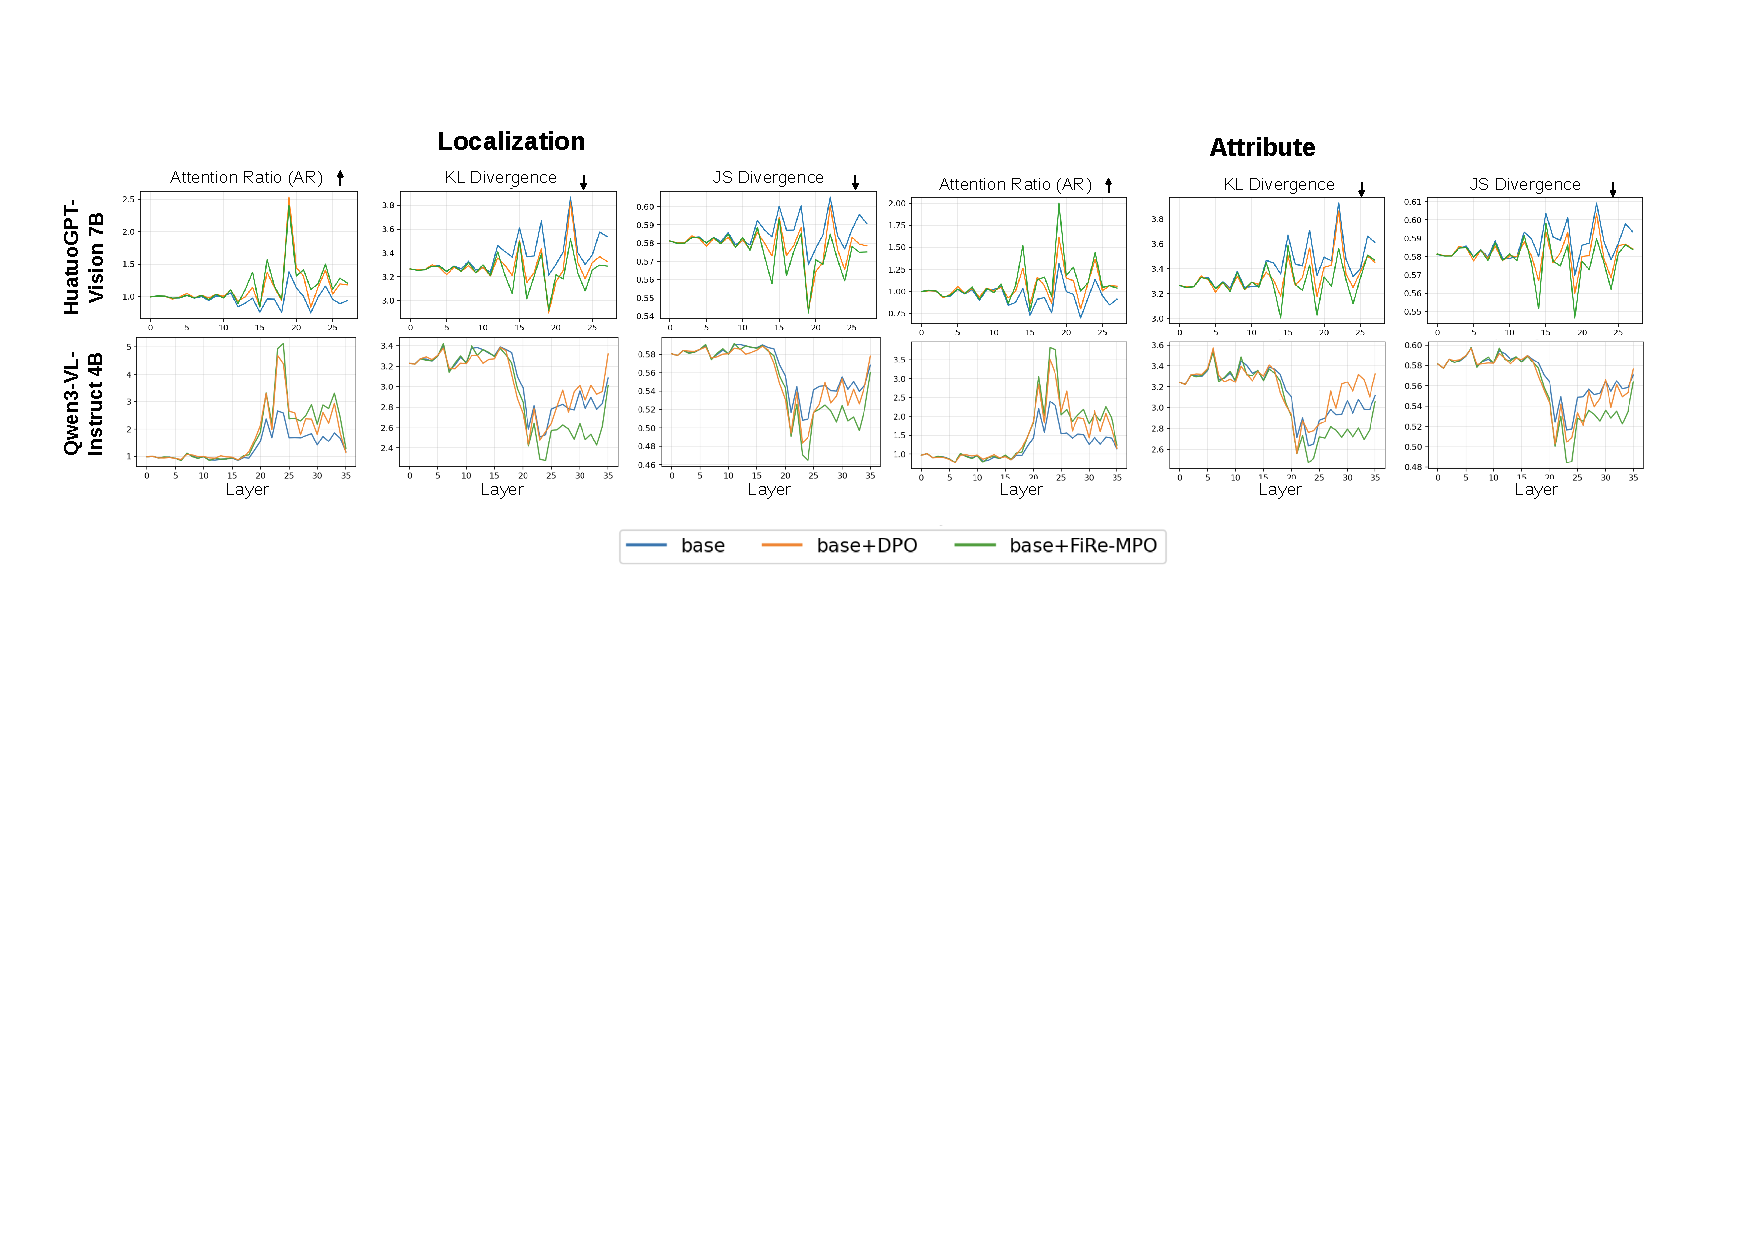
\includegraphics[width=\textwidth]{visual-attention.pdf}
        \caption{\ourloss{} shows superior visual grounding compared to base models and DPO alignment. Attention Ratio (higher is better), KL divergence, and JS divergence (both lower is better) are computed per decoder layer on the VGMED Localization and Attribute subsets, for both backbones.}
        \label{fig:visual_attention}
    \end{figure}
}

Table~\ref{tab:results_loss_updated} establishes that \ourloss{} answers more questions correctly. It does not establish \emph{why}, and Section~\ref{sec:ana:grounding} argued that a purely textual objective can raise accuracy without improving grounding at all. Figure~\ref{fig:visual_attention} tests the mechanism directly, by measuring where the model attends rather than what it outputs.

The figure provides layer-wise analysis of visual grounding on localization and attribute tokens. Across both backbones, the baseline unaligned models (\textit{base}) and standard sequence-level DPO alignment exhibit clear limitations in their internal layer representations, showing lower AR values in deeper layers and weaker alignment to clinically relevant localization and attribute information. In contrast, \ourloss{} demonstrates stronger visual grounding and more controlled distributional alignment across both the specialized \texttt{HuatuoGPT-Vision-7B} and the general-purpose \texttt{Qwen3-VL-4B-Instruct} backbones. Enabled by the fine-grained image preference construction pipeline, the model progressively shifts attention toward diagnostically relevant localization and attribute tokens while maintaining lower KL and JS divergence throughout the network.

This behaviour becomes particularly evident in the deeper layers, where the separation between \ourloss{} and the baseline methods is most pronounced, suggesting that the model relies more consistently on clinically relevant visual evidence when forming its final predictions. The depth-dependence is itself informative: early layers are dominated by generic visual processing that alignment does not touch, while the later layers are where the model commits to an answer. A grounding improvement that appears only in those later layers is consistent with the objective changing how visual evidence is \emph{used} at decision time rather than how it is encoded --- which is what one would expect given that the vision tower is frozen throughout (Section~\ref{sec:met:implementation}).

The DPO curves are the important control. DPO improves accuracy over the base model on several splits, yet its grounding profile tracks the unaligned base model closely. This is direct evidence for the claim in Section~\ref{sec:ana:grounding} that textual preference optimization can buy accuracy through linguistic association rather than through improved use of visual evidence.

Grounding is measured on the VGMED SLAKE subset, and the models evaluated here are the SLAKE-aligned checkpoints. This scope is imposed by the benchmark rather than chosen: the protocol requires per-question region annotations, which VGMED provides only for the SLAKE images it curates, so there is no corresponding grounding evaluation for VQA-RAD or IU-Xray.

\subsection{Training Dynamics}
\label{sec:res:dynamics}

\begin{figure}[t]
    \centering
    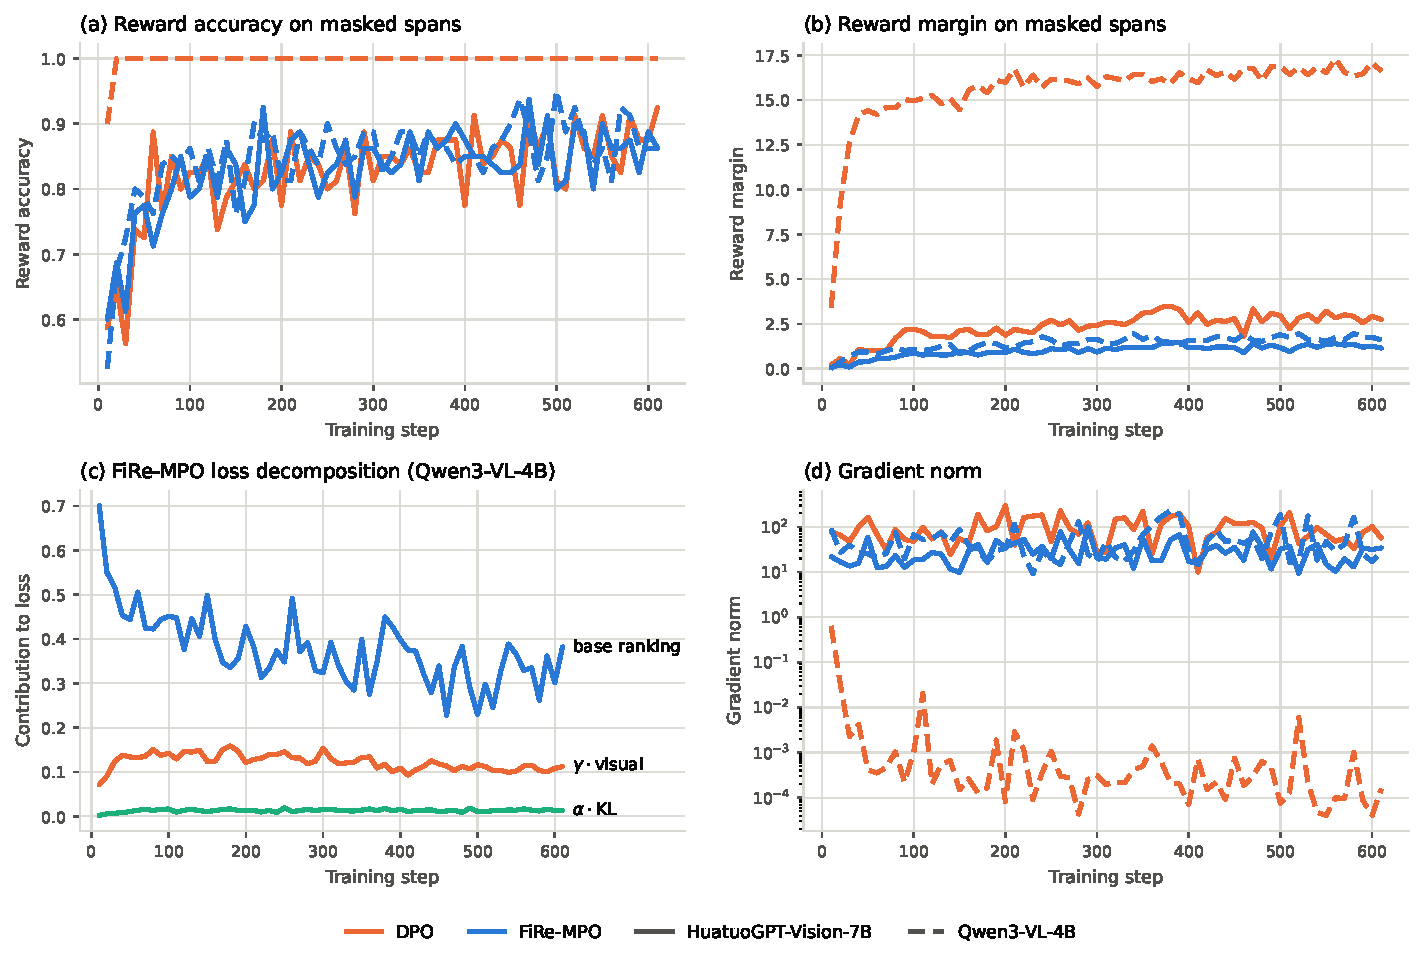
\includegraphics[width=\textwidth]{training_dynamics.pdf}
    \caption{Training dynamics on SLAKE, from the optimizer logs of the aligned runs. Colour encodes the method and line style the backbone. (a) Reward accuracy and (b) reward margin on the masked spans; (c) the three terms of the \ourloss{} objective, scaled by the coefficients with which they enter Equation~\ref{eq:firempo-total}; (d) gradient norm on a logarithmic scale. The Qwen3 DPO run (orange, dashed) saturates its preference objective within roughly fifty steps and its gradients then collapse by six orders of magnitude.}
    \label{fig:training_dynamics}
\end{figure}

Figure~\ref{fig:training_dynamics} examines the optimization itself rather than its end product, and it makes the reward-hacking argument of Section~\ref{sec:ana:reward-hacking} visible in a second, independent way.

\textbf{Saturation of the preference objective.} Panels (a) and (b) show the Qwen3 DPO run reaching a reward accuracy of exactly $1.0$ within about fifty steps and holding it for the remaining five hundred, while its reward margin climbs to roughly $17$ and plateaus. Perfect separation of every preference pair in the corpus after a twelfth of one epoch does not indicate that a hard clinical distinction has been learned; it indicates that the model found a feature that separates the pairs trivially. The \ourloss{} runs, whose pairs are stylistically matched by construction, sit at $0.80$--$0.90$ accuracy with margins near $1.5$ throughout --- the profile of an objective that remains difficult because the only available signal is the clinical one.

\textbf{The consequence for optimization.} Panel (d) shows what saturation costs. Because the DPO loss is $-\log\sigma(\cdot)$ of the margin, a margin of $17$ places the objective in a region where its gradient is vanishingly small. The Qwen3 DPO gradient norm falls from order $10^{-1}$ to order $10^{-4}$ within the first fifty steps and never recovers, meaning the run spends more than $90\%$ of its budget making essentially no parameter updates. This is a mechanistic account of the flat medical accuracy in Figure~\ref{fig:reward_hacking_analysis}: the model is not failing to learn the clinical distinction because the distinction is hard, but because it stopped learning anything once the stylistic shortcut had saturated the objective. The corresponding row of Table~\ref{tab:results_loss_updated} --- Qwen3 + DPO, the only aligned row that scores \emph{below} its own base model on average ($62.73$ versus $63.24$) --- is the downstream result. All \ourloss{} runs maintain gradient norms in the $10^{1}$--$10^{2}$ range for the entire epoch.

\textbf{The size of the KL term.} Panel (c) decomposes the \ourloss{} objective into its three terms, each scaled by the coefficient with which it actually enters Equation~\ref{eq:firempo-total}. The base ranking loss dominates, falling from $0.70$ to about $0.35$. The visual term contributes roughly $0.11$ after scaling by $\gamma = 0.1$, and the bidirectional KL contributes only about $0.015$ after scaling by $\alpha = 0.01$ --- around $4\%$ of the total. That the smallest term by two orders of magnitude is also the one whose removal costs $22$ points of GREEN score (Section~\ref{sec:res:abl-kl}) is worth stating plainly: the regularizer does not work by contributing loss, it works by constraining the direction of the update.

\subsection{Ablation: Bidirectional KL Regularization}
\label{sec:res:abl-kl}

We ablate the three core design choices of \ourloss{} on \texttt{HuatuoGPT-Vision-7B}.

\begin{table}[ht]
\centering
\small
\caption{Impact of forward and reverse KL regularization across medical VQA and report-generation benchmarks.}
\label{tab:regularizer}
\begin{tabular}{lcccc}
\toprule
\textbf{Metric} & \textbf{SLAKE} & \textbf{VQA-RAD} & \textbf{IU-Xray} & \textbf{Average} \\
\midrule
\ourloss{} (Ours) & \textbf{68.14} & {60.31} & \textbf{80.70} & \textbf{69.72}\\
\midrule
w/o Reverse KL & 65.97 & 59.65 & 78.84 & 68.15 \\
w/o Forward KL & 66.35 & 59.65 & 80.98 & 68.99  \\
w/o KL         & 65.40 & \textbf{60.75} & 58.42 & 61.52\\
\bottomrule
\end{tabular}
\end{table}

Table~\ref{tab:regularizer} evaluates the contribution of the forward and reverse KL components. Removing the KL regularizer entirely (\emph{w/o KL}) leads to the largest performance drop on IU-Xray ($80.70\%$ to $58.42\%$). This suggests that regularization plays an important role in stabilizing optimization, especially for long-form report generation. As noted in Section~\ref{sec:res:main}, this configuration \emph{is} MASK-DPO: the localized reward is retained and only $\alpha$ is set to zero, so the row simultaneously serves as an ablation of our regularizer and as the MASK-DPO baseline of Table~\ref{tab:results_loss_updated}. The missing regularizer, not the localized rewards, is what breaks that baseline on reports.

The two KL terms contribute differently, and in the directions the analysis of Section~\ref{sec:ana:kl} predicts. Removing the reverse KL term (\emph{w/o Reverse KL}) reduces performance across all three benchmarks, lowering SLAKE from $68.14\%$ to $65.97\%$, VQA-RAD from $60.31\%$ to $59.65\%$, and IU-Xray from $80.70\%$ to $78.84\%$. This is the tail-suppression effect: without the mode-seeking term, spuriously fluent but clinically incorrect continuations retain probability mass. In contrast, removing the forward KL term (\emph{w/o Forward KL}) primarily affects the VQA tasks, reducing SLAKE to $66.35\%$ and VQA-RAD to $59.65\%$, while IU-Xray is essentially unchanged ($80.98\%$). This asymmetry is consistent with forward KL's role as a coverage safeguard: open-ended question answering draws on the breadth of the base model's clinical knowledge, whereas report generation follows a comparatively narrow template where coverage matters less.

Taken together, these results indicate that the full bidirectional formulation provides the most consistent performance across clinical settings that require both detailed report generation and open-ended visual question answering. Notably, no single variant wins everywhere --- \emph{w/o KL} is best on VQA-RAD and \emph{w/o Forward KL} is marginally best on IU-Xray --- but only the full formulation avoids a severe failure on any benchmark.

\subsection{Ablation: Visual-Contrastive Preference Pairs}
\label{sec:res:abl-visual}

\begin{table}[ht]
\centering
\small
\begin{minipage}[t]{0.48\textwidth}
    \centering
    \caption{Comparison of image corruption strategies used for visual preference construction.}
    \label{tab:corruption}
    \resizebox{\linewidth}{!}{
        \begin{tabular}{lcccc}
        \toprule
        \textbf{Corruption Type} & \textbf{SLAKE} & \textbf{VQA-RAD} & \textbf{IU-Xray} & \textbf{Avg.} \\
        \midrule
        Lesion-Based & \textbf{68.14} & \textbf{60.31} & \textbf{80.70} & \textbf{69.72}\\
        Cropped & 56.13 & 58.76 & 70.13 &  61.67\\
        Image Level Noise & 66.35 & 59.65 & 79.10 & 68.37\\
        Full Black         & 66.72 & 55.28 & 60.22 & 60.74 \\
        \bottomrule
        \end{tabular}
    }
\end{minipage}
\hfill
\begin{minipage}[t]{0.48\textwidth}
    \centering
    \caption{Ablation of visual preference formulations.}
    \label{tab:visual_ablation}
    \resizebox{\linewidth}{!}{
        \begin{tabular}{lcccc}
        \toprule
        \textbf{Metric} & \textbf{SLAKE} & \textbf{VQA-RAD} & \textbf{IU-Xray} & \textbf{Avg.} \\
        \midrule
        \ourloss{} (Ours) & \textbf{68.14} & \textbf{60.31} & 80.70 & \textbf{69.72}\\
        \midrule
        w/o visual pref. & 67.48 & 58.76 & \textbf{81.79} & 69.34 \\
        + v1 ($v, q, y^+ \succ v', q, y^+$) & 63.05 & 58.09 & 77.73 & 66.29 \\
        + v2 ($v, q, y^+ \succ v', q, y^-$) & 65.60 & 59.64 & 79.48 & 68.24 \\
        \bottomrule
        \end{tabular}
    }
\end{minipage}
\end{table}

Tables~\ref{tab:corruption} and~\ref{tab:visual_ablation} evaluate both the image corruption strategy and the visual preference formulation.

\textbf{Corruption granularity.} Table~\ref{tab:corruption} compares different image corruption strategies. Lesion-based corruption achieves the strongest overall performance, outperforming global perturbations such as cropping, image-level noise, and full-image masking across all three benchmarks. The largest gaps are observed relative to cropped images on SLAKE ($68.14\%$ vs.\ $56.13\%$) and fully blacked-out images on IU-Xray ($80.70\%$ vs.\ $60.22\%$).

The ordering of the alternatives is itself instructive. Image-level noise --- the same perturbation as the lesion-based variant, applied globally --- is the closest competitor at $68.37\%$, confirming that the mechanism is genuinely about \emph{where} the corruption is applied rather than what kind it is. Cropping and full blacking perform far worse, and for a reason worth naming: both produce an image that is trivially identifiable as degraded. The model can learn to detect the corruption itself and condition on that, rather than learning to depend on the lesion. Lesion-targeted noise leaves a plausible-looking radiograph in which only the diagnostically decisive region has been destroyed, so the only way to satisfy the objective is to actually attend to that region. These results support the central design choice of \ourloss{}: it teaches the model to anchor its clinical assertions to specific anatomical regions, effectively penalizing lucky hallucinations that lack authentic visual grounding.

\textbf{Preference direction.} Removing visual preferences entirely (Table~\ref{tab:visual_ablation}) reduces performance on the VQA benchmarks, lowering SLAKE from $68.14\%$ to $67.48\%$ and VQA-RAD from $60.31\%$ to $58.76\%$, although IU-Xray improves slightly to $81.79\%$. We further compare the two natural alternative formulations. Both perform worse than the proposed dual-constraint design, with the largest degradation observed for v1, where SLAKE decreases to $63.05\%$ and IU-Xray to $77.73\%$.

The gap between v1 and the proposed formulation is the clearest evidence for the reversal argument of Section~\ref{sec:met:ranking}. Variant v1 merely prefers the correct answer under the clean image over the same answer under the corrupted image; it never tells the model what it \emph{should} do when evidence is missing. Variant v2 is intermediate. Only the full formulation flips the preference under $v'$, and it is the strongest. These results indicate that contrasting clean and corrupted images alone is insufficient: the model also benefits from explicitly learning that a clinically specific answer should not be preferred when the supporting visual evidence has been removed.

\subsection{Ablation: On-Policy Response Editing}
\label{sec:res:abl-style}

\afterpage{
    \begin{figure}[t]
        \centering
        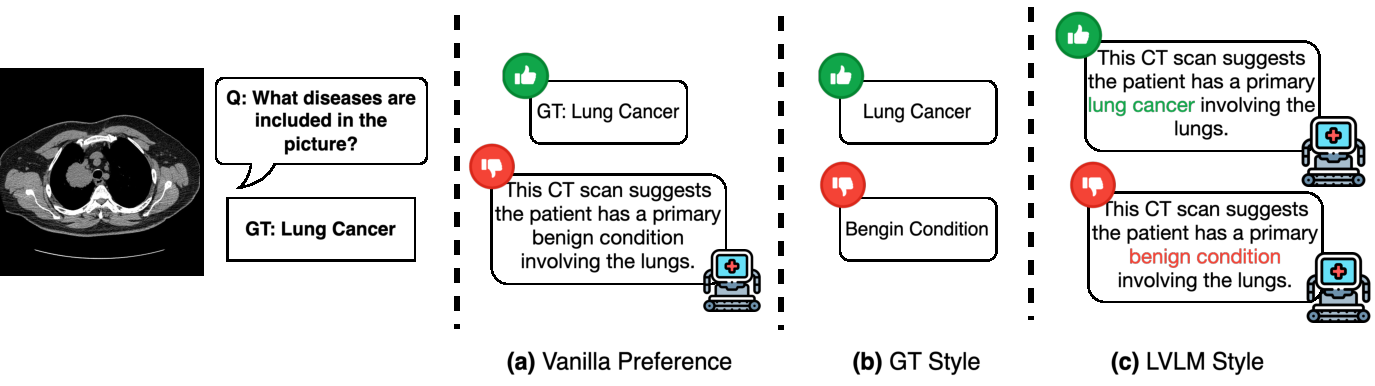
\includegraphics[width=\textwidth]{framework-examples.pdf}
        \caption{Preference-pair construction used in the textual-style ablation. Vanilla preference learning compares the model output directly against the SFT ground truth, creating a large stylistic gap between the rejected and preferred responses. GT-style preference pairs preserve this off-policy mismatch: the preferred answer is short and reference-like, while the rejected answer remains model-like. Our LVLM-style construction edits only the clinically incorrect span while preserving the model's original response style. This isolates the preference signal to clinical factuality rather than surface-level formatting, and corresponds directly to the ablation in Table~\ref{tab:pair_ablation}.}
        \label{fig:examples-fig}
    \end{figure}
}

\begin{table}[ht]
\centering
\small
\caption{Comparison of preference-pair construction strategies on medical VQA benchmarks. Cl, Op, and Ov denote closed-ended, open-ended, and overall performance, respectively.}
\label{tab:pair_ablation}
\begin{tabular}{l | ccc | ccc}
\toprule
& \multicolumn{3}{c|}{\textbf{SLAKE}} & \multicolumn{3}{c}{\textbf{VQA-RAD}} \\
\textbf{Models} & \textbf{Cl} & \textbf{Op} & \textbf{Ov} & \textbf{Cl} & \textbf{Op} & \textbf{Ov} \\
\midrule
Style Agnostic & 73.63 & 47.77 & 56.64 & 70.88 & 38.94 & 57.42 \\
GT Style & \textbf{80.76} & 52.36 & 62.11 & \textbf{73.56} & \textbf{44.21} & \textbf{61.20} \\
LVLM Style & 79.40 & \textbf{55.38} & \textbf{63.62} & 71.65 & 39.47 & 58.09 \\
\bottomrule
\end{tabular}
\end{table}

Figure~\ref{fig:examples-fig} illustrates the three pair-construction strategies evaluated in Table~\ref{tab:pair_ablation}. The style-agnostic setting (vanilla preference learning), which does not explicitly control for stylistic differences between preferred and rejected responses, performs worst across both datasets, achieving overall scores of $56.64\%$ on SLAKE and $57.42\%$ on VQA-RAD. This indicates that the quality of the preference pairs plays a substantial role in downstream alignment performance.

Both GT Style and LVLM Style substantially improve over the style-agnostic baseline, suggesting that preserving coherent response structure during preference construction is beneficial. In the \texttt{GT Style} (off-policy ground truth) setting, the preferred response is written in the style of the supervised reference, while the rejected response remains in the model's own style. In contrast, the \texttt{LVLM Style} (on-policy) approach edits only the clinically incorrect span while preserving the model's original syntax and verbosity. As a result, the preferred and rejected responses remain closer in style and differ primarily in clinical content rather than surface-level formatting. This makes preference learning less susceptible to stylistic shortcuts, where the model can increase the preference margin by imitating the form of the ground-truth response rather than correcting the underlying clinical error.

The result requires an honest reading, because it is the one place where the evidence is mixed. LVLM Style wins overall on SLAKE ($63.62$ versus $62.11$), driven by a large gain on open-ended questions ($55.38$ versus $52.36$), but GT Style wins on VQA-RAD across all three columns. The split follows the response-length pattern seen throughout: the on-policy construction helps most where responses are long and the style gap is therefore largest, and least on VQA-RAD, whose answers are short enough that on-policy and reference styles nearly coincide. A second factor is that VQA-RAD is the smallest corpus in the study at $1{,}786$ pairs, so its measurements are the least stable.

\subsubsection{Measuring the Stylistic Gap Directly}
\label{sec:res:style-gap}

The argument above rests on a claim about the \emph{data} --- that GT-Style pairs differ systematically in style while LVLM-Style pairs do not --- and that claim can be verified without training anything. Table~\ref{tab:style_gap} measures it directly over the preference corpora.

\begin{table}[ht]
\centering
\small
\caption{Stylistic separation between preferred and rejected responses under each construction, measured over the HuatuoGPT-Vision-7B preference corpora. Lengths are in whitespace tokens. $|\Delta\text{len}|$ is the mean \emph{paired} absolute length difference, and \emph{within 2} is the fraction of pairs whose two responses differ by at most two tokens. Edit distance is one minus the word-level sequence similarity, so $0$ means identical and $1$ fully disjoint.}
\label{tab:style_gap}
\begin{tabular}{llrrrrr}
\toprule
\textbf{Dataset} & \textbf{Construction} & \textbf{len($y^+$)} & \textbf{len($y^-$)} & $\mathbf{|\Delta\text{len}|}$ & \textbf{within 2} & \textbf{edit dist.} \\
\midrule
\multirow{3}{*}{SLAKE}
 & Style Agnostic & 1.7  & 1.9  & 0.6  & 94.4\% & 0.894 \\
 & GT Style       & 1.7  & 13.5 & 11.8 & 1.0\%  & 0.978 \\
 & LVLM Style     & 13.1 & 13.5 & 1.3  & 88.1\% & 0.210 \\
\midrule
\multirow{3}{*}{VQA-RAD}
 & Style Agnostic & 1.6  & 1.9  & 0.6  & 93.8\% & 0.921 \\
 & GT Style       & 1.6  & 13.8 & 12.2 & 0.1\%  & 0.980 \\
 & LVLM Style     & 13.3 & 13.8 & 1.6  & 86.7\% & 0.198 \\
\bottomrule
\end{tabular}
\end{table}

The measurement makes the shortcut concrete. Under GT Style, the preferred response averages $1.7$ tokens against the rejected response's $13.5$, and only $1.0\%$ of pairs are within two tokens of each other. A classifier with no access to clinical content could separate $99\%$ of these pairs on length alone, and the word-level edit distance of $0.978$ confirms that the two responses share almost no surface material. This is precisely the spurious signal that Section~\ref{sec:ana:reward-hacking} argued the model would exploit in preference to the clinical distinction, and it is far easier to learn than the diagnosis.

Under LVLM Style the situation inverts. The two responses are nearly identical in length --- $88.1\%$ of pairs differ by at most two tokens --- and the edit distance falls to $0.210$, meaning roughly four fifths of the two responses is shared verbatim. What remains is the edited clinical span. A model cannot raise its preference margin here without engaging with the clinical content, because there is no other systematic difference to exploit.

Style Agnostic is instructive as the third point. Its pairs are also well matched in length ($94.4\%$ within two tokens), yet it performs worst in Table~\ref{tab:pair_ablation}. Its edit distance of $0.894$ explains why: the construction retains only the masked spans, so the two responses are short and almost entirely disjoint, and the model sees the corrected phrase stripped of the sentence that gives it meaning. Matching style is therefore necessary but not sufficient --- the clinical correction must remain embedded in the surrounding response for the preference to be informative.

Taken together with Table~\ref{tab:pair_ablation}, this supports a more precise statement than the accuracy numbers alone permit. The mechanism claimed in Chapter~\ref{section:analysis} is confirmed to exist in the data at the scale claimed. What the single-run accuracies cannot yet settle is how much of the residual difference between GT Style and LVLM Style is attributable to that mechanism as opposed to run-to-run variation, given that the two orderings disagree between SLAKE and VQA-RAD by margins of one to three points.

\subsection{Hyperparameter Sensitivity}
\label{sec:res:sensitivity}

\ourloss{} introduces three hyperparameters beyond the standard DPO temperature: $\lambda$ (the balance between the two KL directions), $\alpha$ (the weight of the regularizer), and $\gamma$ (the weight of the visual grounding term). All results above use $\lambda = 0.5$, $\alpha = 0.01$, and $\gamma = 0.1$.

The ablations already reported constitute a coarse sensitivity analysis, because each removes a component by driving one of these parameters to an endpoint of its range. Reading them that way, Table~\ref{tab:sensitivity} collects what the experiments establish about each parameter.

\begin{table}[ht]
\centering
\small
\caption{Sensitivity of the average score across the three benchmarks to each loss coefficient, assembled from the ablations of Tables~\ref{tab:regularizer} and~\ref{tab:visual_ablation} on HuatuoGPT-Vision-7B. Each row varies one coefficient with the others held at their defaults. Values marked $^{\dagger}$ are the default configuration.}
\label{tab:sensitivity}
\begin{tabular}{llccc}
\toprule
\textbf{Coefficient} & \textbf{Role} & \multicolumn{3}{c}{\textbf{Average score}} \\
\midrule
\multirow{2}{*}{$\lambda$} & \multirow{2}{*}{forward/reverse KL balance}
  & $\lambda{=}0$ & $\lambda{=}0.5^{\dagger}$ & $\lambda{=}1$ \\
  & & 68.99 & \textbf{69.72} & 68.15 \\
\midrule
\multirow{2}{*}{$\alpha$} & \multirow{2}{*}{KL regularizer weight}
  & $\alpha{=}0$ & $\alpha{=}0.01^{\dagger}$ & \\
  & & 61.52 & \textbf{69.72} & \\
\midrule
\multirow{2}{*}{$\gamma$} & \multirow{2}{*}{visual grounding weight}
  & $\gamma{=}0$ & $\gamma{=}0.1^{\dagger}$ & \\
  & & 69.34 & \textbf{69.72} & \\
\bottomrule
\end{tabular}
\end{table}

Three conclusions are supported, and their strength differs considerably.

The $\lambda$ result is the most informative, because it has an interior point flanked by both endpoints. The default $\lambda = 0.5$ outperforms both pure reverse KL ($68.99$) and pure forward KL ($68.15$), so the optimum is genuinely interior rather than at a boundary. This is the empirical content of the argument in Section~\ref{sec:ana:kl}: a balanced regularizer is not a compromise between two adequate options but the only setting that avoids both failure modes. The curve is also asymmetric --- forward KL alone is the worse endpoint, costing $1.57$ points against $0.73$ for reverse KL alone --- indicating that tail suppression contributes more than coverage preservation at this operating point, which is what one would expect when the objective is factuality.

The $\alpha$ result is the largest effect in the entire study, but it is measured at only two points. Moving from $\alpha = 0$ to $\alpha = 0.01$ is worth $8.20$ points on average, almost all of it on report generation. What these experiments do not establish is the shape of the response between and beyond those points: whether performance is flat across an order of magnitude of $\alpha$, or whether $0.01$ sits on a narrow peak. Given that the regularizer contributes only about $4\%$ of the total loss magnitude (Section~\ref{sec:res:dynamics}), a broad optimum is plausible, but it is not demonstrated here.

The $\gamma$ result is the weakest. The gain from adding the visual term at $\gamma = 0.1$ is $0.38$ points on the average, which is smaller than the differences elsewhere in this chapter that Section~\ref{sec:res:variance} argues are not resolvable by single-run evaluation. The stronger evidence for the visual component is not this coefficient comparison but the preference-formulation ablation in Table~\ref{tab:visual_ablation}, where the alternative formulations v1 and v2 lose $3.43$ and $1.48$ points respectively, and the corruption-strategy comparison in Table~\ref{tab:corruption}, where the gaps reach $8$ points. Those margins are large enough to be informative; the $\gamma$ margin alone is not.

The analysis is therefore coarse: three points for $\lambda$ and two each for $\alpha$ and $\gamma$, all on a single backbone and a single seed. It establishes that the interior $\lambda$ is correct and that $\alpha$ matters enormously, but it does not locate the optimum of any of the three, and the defaults should be read as reasonable settings rather than tuned ones.

\subsection{Which Results the Evidence Supports}
\label{sec:res:variance}

Every number reported in this chapter comes from a single training run. That is standard practice in the preference-optimization literature, but it bounds what may legitimately be concluded, and this section states those bounds explicitly rather than leaving them to the reader.

Two dispersion estimates are available. The GREEN evaluation on IU-Xray reports a per-report standard deviation alongside the mean: $0.7327 \pm 0.4229$ for \ourloss{} against $0.6071 \pm 0.4338$ for DPO. The spread across individual reports is large relative to the difference in means, which is expected for a per-example metric over $590$ test reports, but it shows that the aggregate comparison rests on averaging rather than on a consistent per-case advantage. Separately, the training-dynamics analysis of Section~\ref{sec:res:dynamics} shows the two backbones behaving very differently under the same objective, which is a reminder that a single configuration is not a single point of behaviour.

Against that, the results divide into three tiers.

\textbf{Robust.} Effects of eight points or more, reproduced across both backbones or across independent measurements, and accompanied by a mechanism. The collapse of long-form report generation when the KL regularizer is removed ($22.28$ points on IU-Xray) falls here: it appears twice under two names --- as the MASK-DPO baseline and as the \emph{w/o KL} ablation --- and Section~\ref{sec:res:dynamics} identifies the mechanism. So does the advantage of lesion-targeted over global corruption ($8.05$ points against cropping, $8.98$ against full masking), and the overall gain of \ourloss{} over the base models ($8.50$ and $4.17$ points). The grounding results of Section~\ref{sec:res:grounding} also belong here, being layer-wise curves separated consistently across all $32$ layers and two backbones rather than single scalars.

\textbf{Supported by mechanism, not by margin alone.} Effects of one to three points that would individually be unresolvable, but which are corroborated by an independent measurement of the mechanism they are attributed to. The on-policy construction is the clearest case: its accuracy advantage is $1.51$ points on SLAKE and reverses on VQA-RAD, but the stylistic separation it is supposed to remove is measured directly in Table~\ref{tab:style_gap} and is enormous --- $99\%$ of GT-Style pairs separable on length alone against $12\%$ of LVLM-Style pairs. The mechanism is established even where the accuracy margin is not. The reward-hacking analysis is similar: the accuracy evidence in Figure~\ref{fig:reward_hacking_analysis} is corroborated by the gradient collapse in Figure~\ref{fig:training_dynamics}, which is a six-order-of-magnitude effect rather than a marginal one.

\textbf{Directional only.} Differences below roughly three points with no corroborating measurement. The VQA-RAD Open gain of $+1.05$ on Qwen3, the $0.38$-point average gain from the visual term in Table~\ref{tab:visual_ablation}, and the ordering of \ourloss{} against MASK-DPO on VQA-RAD Closed ($71.26$ against $73.18$) are in this tier. These are reported for completeness and should be read as consistent with the thesis rather than as evidence for it. Notably, no claim in Chapter~\ref{section:conclusion} depends on any of them.

The natural strengthening of this analysis is seed replication with paired significance testing over per-question outcomes, which would convert the third tier into either the second or a null result. That is a matter of compute rather than of methodology: a three-seed replication of the four methods across both backbones is $24$ training runs, which at the measured cost of Table~\ref{tab:cost} is roughly a day of single-GPU time, and the peak memory reported there rules out running them concurrently on one device.

\subsection{Qualitative Analysis}
\label{sec:res:qualitative}

The quantitative results are complemented by inspection of individual outputs; a representative set is collected in Appendix~\ref{app:cases}. Three behavioural patterns recur.

\textbf{Verbosity collapse under DPO.} On many questions the DPO-aligned model answers with a bare noun phrase --- ``Lung'', ``No'', ``Left'' --- discarding the explanatory framing of the base model entirely. This is the generation-length effect of Figure~\ref{fig:reward_hacking_analysis} visible case by case. \ourloss{}-aligned outputs retain the base model's explanatory register while correcting the clinical content, which is the intended consequence of on-policy construction. The distinction matters clinically: a bare label is not auditable, whereas a stated finding with its supporting observation can be checked by the reader.

\textbf{Correction of confident hallucinations.} On cases where the base model asserts a finding that is not present --- for instance, describing bilateral lung consolidation on a radiograph where the ground truth is negative --- \ourloss{} produces an explicit negative statement that names the evidence for it, whereas the base model produces a fluent multi-sentence elaboration of the non-existent finding.

\textbf{Residual errors are inherited.} Where the base model's perceptual reading is wrong rather than its verbalization, alignment does not always recover it. This is consistent with the frozen vision tower: the objective can change how visual evidence is weighed, but it cannot supply evidence the encoder never extracted.

Figures~\ref{fig:case1}--\ref{fig:case7} in Appendix~\ref{app:cases} show these three patterns across both backbones and all three benchmarks. They are offered as illustration of the mechanisms established quantitatively above, rather than as independent evidence; the cases in Appendix~\ref{app:cases} were selected to be representative of behaviours the aggregate metrics already measure.

\section{Discussion, Limitations, and Conclusion}
\label{section:conclusion}

\subsection{Discussion}
\label{sec:con:discussion}

The results in Chapter~\ref{section:results} support the thesis statement, but it is worth being precise about which parts of the argument the evidence actually carries and which remain provisional.

\textbf{The three failure modes are coupled, not independent.} This was the central claim of Chapter~\ref{section:analysis}, and the ablations bear it out in a specific way. Fine-grained rewards without a regularizer do not merely fail to help --- they actively destabilize long-form generation, as both the MASK-DPO baseline and the \emph{w/o KL} ablation show by collapsing on IU-Xray to well below the unaligned base model. Conversely, the regularizer contributes only about $4\%$ of the total loss magnitude (Figure~\ref{fig:training_dynamics}) yet its removal costs $22$ points of GREEN score. A component's importance is not proportional to its contribution to the objective value; the KL term works by constraining the direction of the update, not by supplying loss. Treating these design choices as an independent menu, as an ablation table implicitly invites, would misread the result.

\textbf{Reward hacking is an optimization pathology, not only an evaluation artifact.} The most useful new evidence in this thesis is the training-dynamics analysis of Section~\ref{sec:res:dynamics}. That off-policy DPO scores poorly on medical accuracy was already known. What the optimizer logs add is the mechanism: reward accuracy reaches $1.0$ within roughly fifty steps, the margin saturates near $17$, and the gradient norm then falls to order $10^{-4}$ and stays there for the remaining ninety percent of training. The model does not fail to learn the clinical distinction because the distinction is hard; it stops learning anything at all once the stylistic shortcut has driven the logistic loss into its flat region. This reframes the remedy. On-policy construction is valuable not merely because it produces a better-calibrated preference signal, but because it keeps the objective difficult enough that optimization continues.

\textbf{Grounding is separable from accuracy, and both need to be measured.} The layer-wise analysis shows DPO improving accuracy on several splits while its attention profile tracks the unaligned base model. Had this study reported only Table~\ref{tab:results_loss_updated}, it would have concluded that DPO partially works. The grounding measurements show that on several splits it works for the wrong reason. For a clinical system, the distinction is not academic: a model that is right by prior will fail on the atypical case, which is the case where it is most needed.

\textbf{Where the gains concentrate is itself a finding.} Improvements are consistently larger on open-ended questions and report generation than on closed questions. This is what the diagnosis predicts --- a short binary answer is already approximately fine-grained, so localizing the reward buys little --- and it is a useful guide to where these techniques should be applied. It also suggests that the headline average understates the effect in the regime that matters most clinically, since free-text reporting is where hallucination is both most likely and most consequential.

\subsection{Limitations}
\label{sec:con:limitations}

While \ourloss{} demonstrates consistent gains across medical VQA and report generation benchmarks, several limitations remain.

\textbf{Dependence on external models.} The on-policy preference construction pipeline depends on external models --- \texttt{GPT-4o-mini} for VQA extraction, \texttt{Gemini 3 Flash Preview} for report refinement, and MedSAM3-v1 for lesion segmentation --- introducing potential error propagation when the task is more niche. An extraction error silently produces a mislabelled preference pair, and there is currently no audit of how often this occurs.

\textbf{Reliance on segmentation quality.} The lesion-targeted corruption strategy requires reliable segmentation masks, which may be unavailable or imprecise for rare pathologies or underrepresented imaging modalities. Section~\ref{sec:exp:corpus} quantifies this: only $64.0\%$ of SLAKE records and $56.0\%$ of VQA-RAD records receive genuinely lesion-targeted corruption, the remainder falling back to global noise because no concept prompt could be extracted or because MedSAM3 returned no detection. The reported benefit of lesion-level corruption is therefore achieved with roughly $40\%$ of each VQA corpus receiving the weaker global treatment. A further restriction is structural rather than incidental: report generation admits no single query-relevant region, so IU-Xray uses holistic noise throughout and the visual term there tests dependence on the image as a whole rather than on a specific finding.

\textbf{Restriction to radiology.} Our evaluation is confined to radiology, and it remains an open question whether the framework generalizes to other clinical imaging domains such as pathology, dermatology, or ophthalmology, which exhibit substantially different visual grounding characteristics. All evaluation is additionally in-distribution, on the test split of the dataset the model was aligned on.

\textbf{Frozen perceptual front end.} Because the vision encoder and projector remain frozen, the method can change how visual evidence is weighed but cannot supply evidence the encoder never extracted. Errors rooted in perception rather than verbalization are outside its reach, as the qualitative analysis in Section~\ref{sec:res:qualitative} notes.

\subsection{Broader Impact}
\label{sec:con:impact}

The broader impact of this work lies in its potential to enhance the reliability and factual consistency of AI-driven medical diagnostics. Improved alignment between model outputs and clinically decisive visual evidence could reduce hallucinated findings in radiology reports and medical VQA, supporting clinicians in time-sensitive diagnostic workflows.

Ethical considerations remain paramount. The aligned model can still suffer from critical errors inherited from the base model, and improvements in fluency and apparent confidence may make residual errors \emph{harder} for a reader to detect rather than easier --- a risk this work shares with any method that improves surface quality alongside factuality. Responsible use requires safeguards against over-reliance on AI-generated medical advice in high-stakes decision-making contexts. The observation in Section~\ref{sec:res:qualitative} that DPO-aligned models collapse toward bare labels while \ourloss{} preserves explanatory framing is relevant here: a stated finding with its supporting observation can be audited by a clinician, whereas a bare label cannot.

Future societal benefits may include reduced diagnostic errors, improved radiological workflow efficiency, and broader access to AI-assisted clinical interpretation in resource-limited settings. These gains must be pursued alongside rigorous prospective validation and ongoing ethical oversight to ensure that advances in fine-grained medical alignment genuinely serve the best interests of patients and healthcare providers.

\subsection{Future Work}
\label{sec:con:future}

Several directions follow directly from the limitations above.

\textbf{Reducing pipeline dependence.} The extraction and segmentation stages are the framework's most fragile components. Auditing extraction reliability against a human-labelled subset, and replacing or ensembling the segmentation model where masks are unreliable, would both improve quality and quantify the error propagation the current pipeline leaves unmeasured.

\textbf{Iterative and online variants.} The construction is currently applied once, against the initial policy. Because the pipeline is fully automatic, it could be re-run against the aligned model to generate a fresh on-policy corpus, giving an iterative scheme in which the preference distribution tracks the policy. The training-dynamics analysis suggests a natural stopping criterion: iterate while the objective remains unsaturated.

\textbf{Grounding as a training signal.} The attention-based grounding measures are used here purely for evaluation, which keeps them independent of the objective. Incorporating them directly into training is an obvious extension, though it would forfeit that independence and require a separate held-out grounding benchmark.

\textbf{Clinician evaluation.} Ultimately, the claim that these gains are clinically meaningful requires clinician judgement rather than model-based judgement, on a stratified sample with inter-rater agreement reported.

\subsection{Conclusion}
\label{sec:con:conclusion}

This thesis began from an empirical anomaly: preference optimization, which transformed alignment in the general domain, yields inconsistent gains over supervised fine-tuning on medical vision-language tasks. We argued that this is not a limitation of preference learning as such, but a consequence of three specific mismatches between the standard formulation and what clinical correctness requires --- a reward too coarse to isolate the decisive spans, a preference construction that confounds clinical content with response style, and an objective with no term tying an assertion to the evidence supporting it. To these we added a fourth consideration, the geometry of the KL regularizer, which governs whether alignment suppresses fluent-but-wrong continuations or merely preserves the base model's coverage.

We presented \ourloss{}, which addresses all four within a single objective: preference pairs constructed by minimally editing the model's own generations so that style is held constant, a fine-grained ranking loss restricted to the clinically divergent spans, a bidirectional token-wise KL regularizer balancing coverage against tail suppression, and a dual-constraint visual term over lesion-corrupted images that reverses the preference when the supporting evidence has been destroyed.

Across two backbones spanning medical-specialized and general-purpose pretraining, and three benchmarks spanning visual question answering and report generation, \ourloss{} outperforms standard DPO and prior fine-grained alignment methods, with an average relative improvement of $10.24\%$. Layer-wise attention analysis shows that the improvement is accompanied by stronger reliance on diagnostically relevant image regions, and controlled ablations isolate the contribution of each component. Analysis of the optimizer logs provides an independent, mechanistic account of stylistic reward hacking, showing an off-policy run saturating its objective within a twelfth of an epoch and ceasing to learn thereafter.

The broader lesson is that alignment techniques do not transfer across domains unexamined. The properties that make DPO attractive --- that it needs only comparisons, and that it reduces to supervised learning on a static dataset --- are the same properties that let it be satisfied by a stylistic shortcut when the comparisons are constructed cheaply. In a domain where correctness is localized to a handful of tokens and depends on evidence the model may not be reading, the objective must be told where to look.


\bibliographystyle{ieeetr}
\bibliography{biblio}

\newpage
\appendix
\addcontentsline{toc}{section}{Appendices}
\section*{Appendices}
\renewcommand{\thesubsection}{\Alph{subsection}}
\setcounter{subsection}{0}

\subsection{\ourloss{} Pseudocode}
\label{app:pseudocode}

The listing below gives the objective of Equation~\ref{eq:firempo-total} in executable form. All log-probability arguments are phrase-level, that is, already restricted to the positions selected by the \texttt{<mask>} spans of Section~\ref{sec:met:data}.

\begin{verbatim}
def FiRe-MPO(
    self,
    # phrase-level logprobs
    chosen_phrase_logps, rejected_phrase_logps,
    ref_chosen_phrase_logps, ref_rejected_phrase_logps,

    # v' visual pair at phrase level
    v_chosen_phrase_logps, v_rejected_phrase_logps,
    ref_v_chosen_phrase_logps, ref_v_rejected_phrase_logps,

    # token logits for phrase-level KL
    chosen_logits, ref_chosen_logits, phrase_mask, ref_phrase_mask,

    has_rejected_image,
    beta, alpha, gamma, lambda,  # hyperparams
):

    # -------- 1) Base phrase preference --------
    # margins computed from phrase-only logprobs
    base_margin = beta * (
        (chosen_phrase_logps - rejected_phrase_logps)
        - (ref_chosen_phrase_logps - ref_rejected_phrase_logps)
    )
    base_loss = -F.logsigmoid(base_margin)  # [B]

    # -------- 2) Visual preference (v' only, phrase-level) --------
    v_margin = beta * (
        (v_chosen_phrase_logps - v_rejected_phrase_logps)
        - (ref_v_chosen_phrase_logps - ref_v_rejected_phrase_logps)
    )
    v_loss = -F.logsigmoid(v_margin)      # [B]

    loss = base_loss + gamma * v_loss

    # -------- 3) token-wise KL --------
    logp_pi  = F.log_softmax(chosen_logits, dim=-1)       # [B,S,V]
    logp_ref = F.log_softmax(ref_chosen_logits, dim=-1)   # [B,S,V]

    # forward KL(ref || pi), then keep phrase positions only
    tkl_tok = (logp_ref.exp() * (logp_ref - logp_pi)).sum(dim=-1)   # [B,S]
    tkl = (tkl_tok * phrase_mask.float()).sum(dim=-1)               # [B]

    # reverse KL(pi || ref), also phrase-only
    rtkl_tok = (logp_pi.exp() * (logp_pi - logp_ref)).sum(dim=-1)   # [B,S]
    rtkl = (rtkl_tok * ref_phrase_mask.float()).sum(dim=-1)         # [B]

    mixed_tkl = lambda * tkl + (1.0 - lambda) * rtkl
    loss = loss + alpha * mixed_tkl

    return loss.mean()
\end{verbatim}

Note that in the visual term, \texttt{v\_chosen} corresponds to $y^-$ and \texttt{v\_rejected} to $y^+$: the preference is reversed under the corrupted image, as required by Equation~\ref{eq:firempo-rank}. The \texttt{has\_rejected\_image} flag masks that term out for records with no corrupted counterpart.

\subsection{Prompt Templates}
\label{app:prompts}

The instructions used for processing the open-ended generated responses are given below. We utilize a multi-stage approach to first evaluate correctness (Stage 1) and then identify and incorporate fine-grained clinical differences (Stage 2).

\begin{figure}[ht]
\centering
\begin{tcolorbox}[colback=boxgray, colframe=black!70, boxrule=0.5pt, arc=0mm, left=8pt, right=8pt, top=8pt, bottom=8pt]
\small \ttfamily
\{Stage 1: Prompt used in VQA answer localization.\} \\
You are evaluating a model's answer to a medical question. \\
\\
Question: \{question\} \\
Correct answer (ground truth): \{answer\} \\
Model's full answer: \{output\} \\
\\
Perform these four steps and respond with a single JSON object only (no other text): \\
\\
1. **answer\_sentence**: The minimal phrase or clause from the model's answer that states the final answer, using the model's exact wording. Preserve the model's language so the final answer is visible in context. Do not include extra clauses that follow. \\
2. **final\_answer**: Locate and extract the final answer to the question from the model's answer. Use as few words as possible (the first occurrence of the conclusive answer). \\
3. **is\_correct**: true if the final answer is correct given the ground truth, false otherwise. \\
4. **opposite\_answer**: Modify the answer sentence as little as possible to make a medically plausible alternative for the question. \\
\\
Respond only with valid JSON in this exact shape: \\
\{"answer\_sentence": "...", "final\_answer": "...", "is\_correct": true or false, "opposite\_answer": "..."\} \\
\\
\\
\{Stage 2: Prompt used in VQA answer difference localization.\} \\
You are given two sentences that are the same except for some phrases. Your task is to identify the phrases in each sentence that differs from the other. \\
\\
Sentence A: \{sentence\_a\} \\
Sentence B: \{sentence\_b\} \\
\\
Wrap only the differing phrases in \texttt{`<mask\>`} \texttt{`</mask\>`} tags. The differing phrases should be as short as possible.
\end{tcolorbox}
\caption{Prompt template used for VQA task answer localization and ground-truth incorporation.}
\label{fig:prompt_stage1}
\end{figure}

\begin{figure}[ht]
\centering
\begin{tcolorbox}[colback=boxgray, colframe=black!70, boxrule=0.5pt, arc=0mm, left=8pt, right=8pt, top=8pt, bottom=8pt]
\small \ttfamily
\{Stage 1: Prompt used in report generation modification\} \\ \\
**Task:** Rewrite **Report A** to make a medically difficult preference pair. \\
\\
**Instruction:** \\
* **Change Logic**: Use the facts in **Report B** to replace a few medical words in Report A to create a fine-grained preferred pair. \\
* **all\_correct**: If all the facts in Report B are already present in Report A, change a few words yourself to make a rejected pair. \\
\\
**Constraints:** \\
* **Structural Locking:** The format of Report A should be preserved. \\
* **Token Parsimony:** At most **two or three words per sentence** can be changed. \\
* **Clinical Significance:** The rejected response should be clinically different from Report A. Changing synonyms (\textit{e.g.} "clear" vs "normal", "healthy" vs "unremarkable") is not accepted. \\
* **Output Format:** Return a JSON object containing keys `all\_correct` and `rewritten\_report\_a`. \\
\\
**Input Data:** \\
* **Report A:** \{report\_a\} \\
* **Report B:** \{report\_b\} \\
\\
\{Stage 2: Prompt used in report generation answer difference localization\} \\ \\
CHEST\_MASK\_PROMPT = """Compare two reports and put the differing phrases inside \texttt{`<mask\>`} \texttt{`</mask\>`} tags. \\
\\
Output: \\
Return **only** a valid JSON object with two keys: `report\_a\_masked` and `report\_b\_masked`. Each key should be a string with the differing phrases wrapped in \texttt{`<mask\>`} \texttt{`</mask\>`} tags. \\
\\
Report A: \\
\{report\_a\} \\
\\
Report B: \\
\{rewritten\_report\_a\} \\
"""
\end{tcolorbox}
\caption{Prompt template used for the report generation task, answer localization and ground-truth incorporation.}
\label{fig:prompt_stage2}
\end{figure}

\clearpage
\subsection{Implementation Details and Asset Licenses}
\label{app:impl}

\begin{table}[ht]
    \caption{Details of training hyperparameters.}
    \label{tab:hyperparams}
    \centering
    \small
    \begin{tabular}{lcc}
        \toprule
        & \textbf{HuatuoGPT-Vision-7B} & \textbf{Qwen3-VL-4B} \\
        \midrule
        Is medically SFT & \checkmark & $\times$ \\
        Trainable module & \multicolumn{2}{c}{LoRA in LLM; everything else kept frozen} \\
        LoRA setup & \multicolumn{2}{c}{rank=128, alpha=256, dropout=0.05} \\
        Learning rate & 1e-6 & 1e-6 \\
        Learning rate scheduler & Cosine & Cosine \\
        Optimizer & AdamW & AdamW \\
        Weight decay & 0.0 & 0.0 \\
        Warmup ratio & 0.0 & 0.0 \\
        Epochs & 1 & 1 \\
        Batch size per GPU & 4 & 4 \\
        Batch size (total) & 8 & 8 \\
        $\beta$ (loss coefficient) & 0.1 & 0.1 \\
        $\alpha$ (loss coefficient) & 0.01 & 0.01 \\
        $\gamma$ (loss coefficient) & 0.1 & 0.1 \\
        $\lambda$ (loss coefficient) & 0.5 & 0.5 \\
        Memory optimization & unsloth & unsloth \\
        \bottomrule
    \end{tabular}
\end{table}

Training was performed on an H100 80GB GPU, while inference utilized two L40s.

\noindent \textbf{Licenses of existing assets used.}
\begin{itemize}
    \item HuatuoGPT-Vision-7B (Apache License 2.0): \url{https://huggingface.co/FreedomIntelligence/HuatuoGPT-Vision-7B}
    \item Qwen3-VL-4B-Instruct (Apache License 2.0): \url{https://huggingface.co/Qwen/Qwen3-VL-4B-Instruct}
\end{itemize}

\clearpage
\subsection{Additional Qualitative Cases}
\label{app:cases}

\begin{figure}[ht]
    \centering
    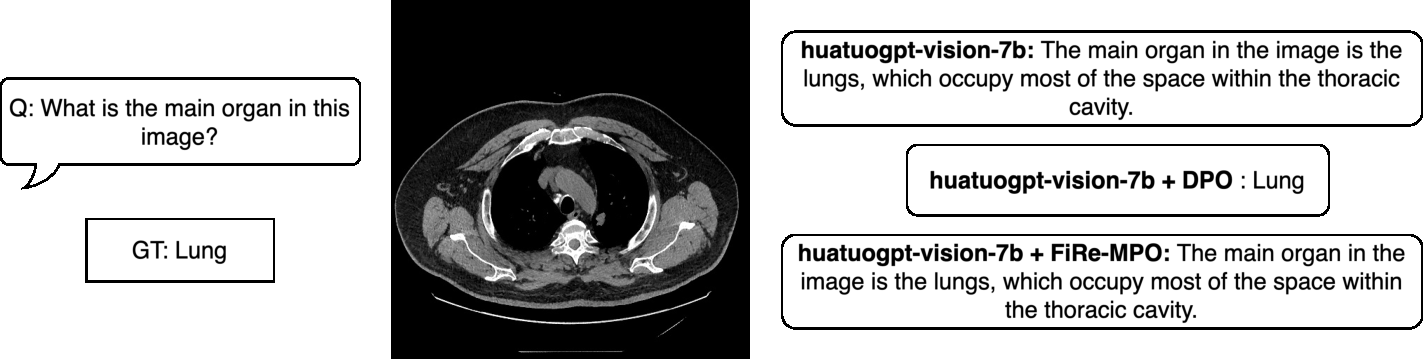
\includegraphics[width=\textwidth]{examples/example1.pdf}
    \caption{Qualitative comparison on organ identification. The DPO-aligned model answers with a bare noun phrase, while \ourloss{} preserves the base model's explanatory register and its clinical content.}
    \label{fig:case1}
\end{figure}

\begin{figure}[ht]
    \centering
    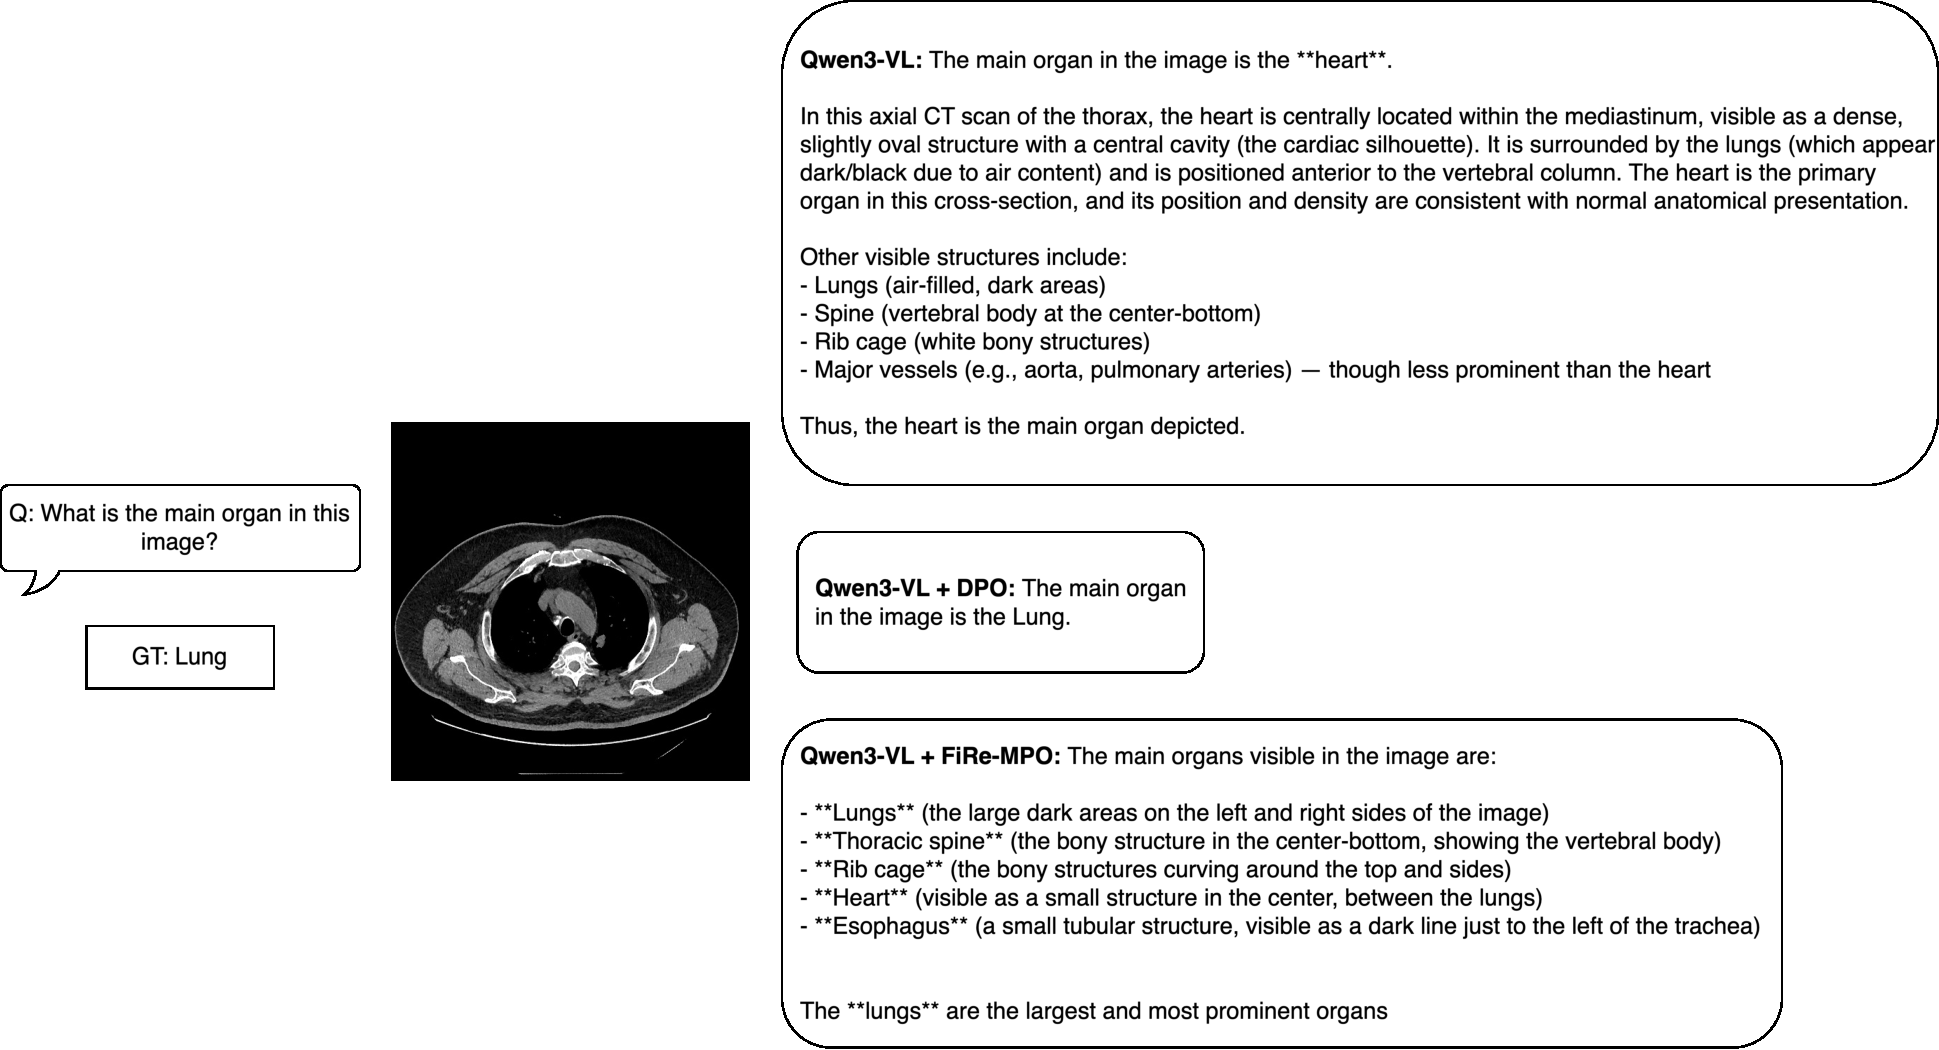
\includegraphics[width=\textwidth]{examples/example2.pdf}
    \caption{Qualitative comparison on a negative finding. The base model elaborates a consolidation that is not present; \ourloss{} produces an explicit negative statement naming the supporting observation.}
    \label{fig:case2}
\end{figure}

\begin{figure}[ht]
    \centering
    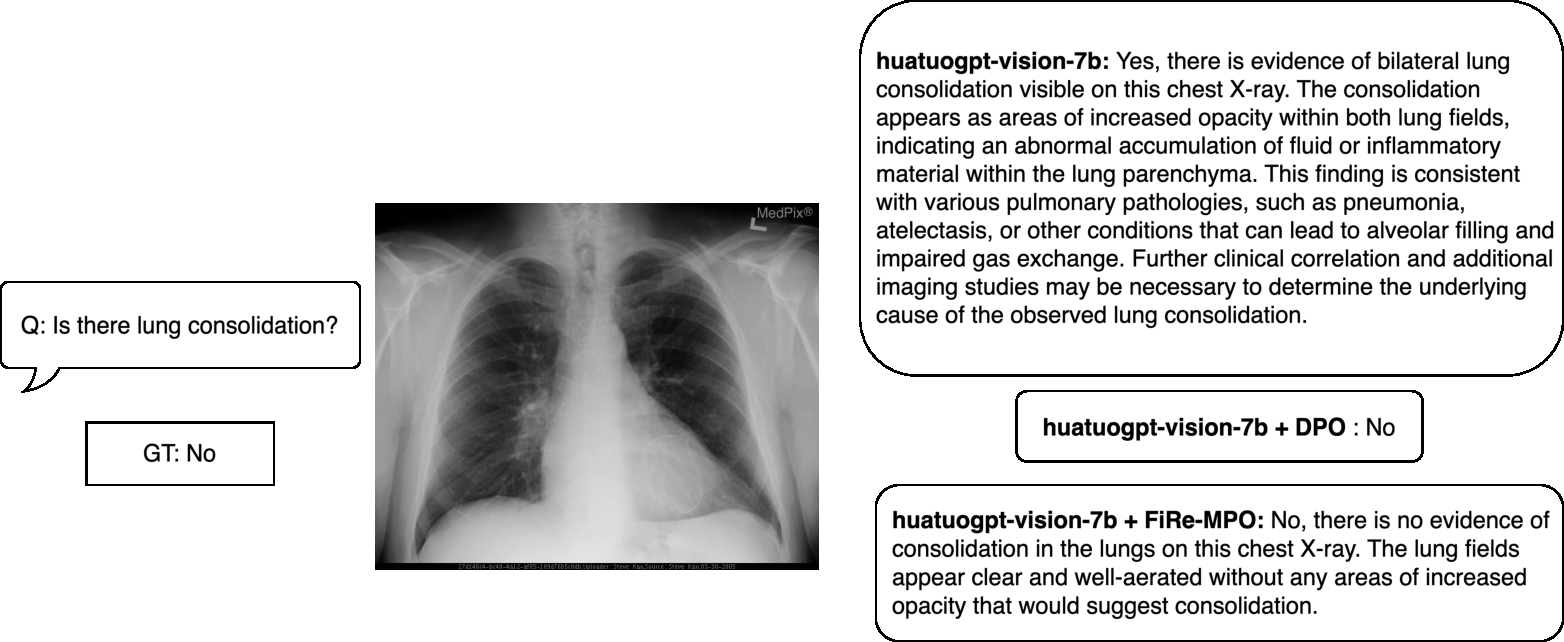
\includegraphics[width=\textwidth]{examples/example3.pdf}
    \caption{Qualitative comparison on preservation of costophrenic angles.}
    \label{fig:case3}
\end{figure}

\begin{figure}[ht]
    \centering
    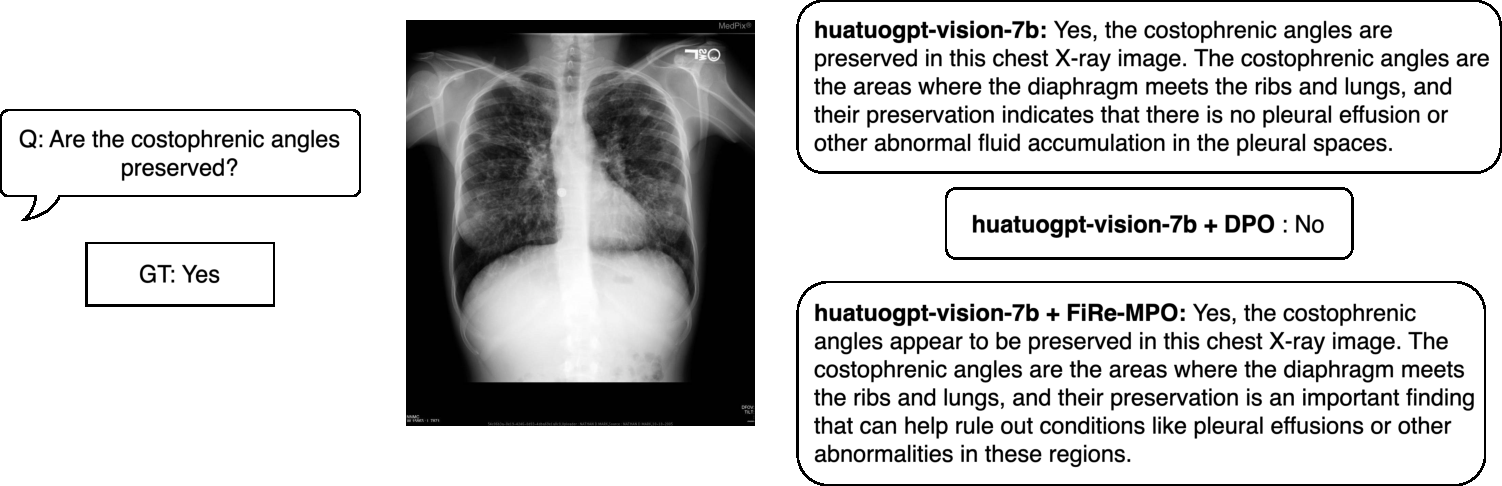
\includegraphics[width=\textwidth]{examples/example4.pdf}
    \caption{Qualitative comparison on lesion attribute description (ring enhancement).}
    \label{fig:case4}
\end{figure}

\begin{figure}[ht]
    \centering
    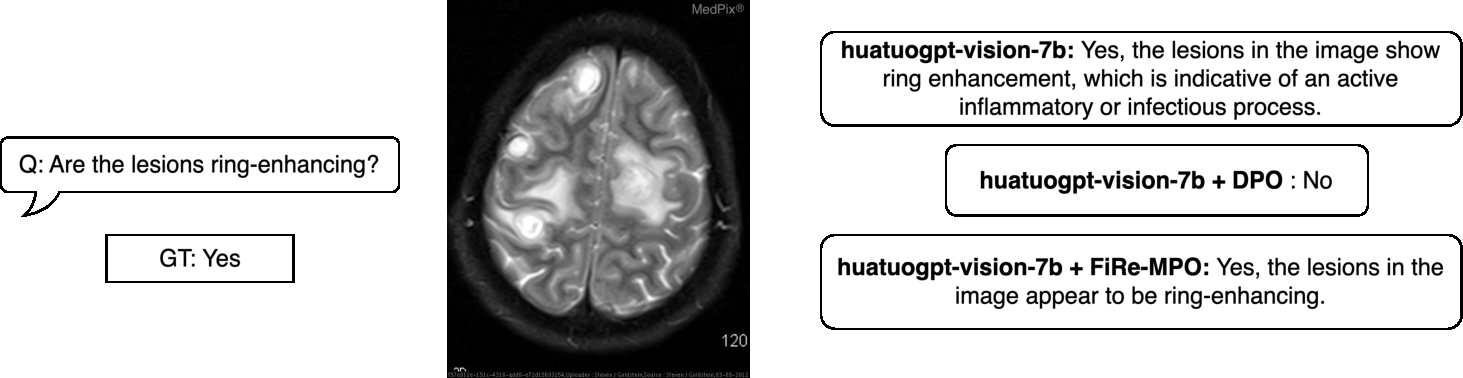
\includegraphics[width=\textwidth]{examples/example5.pdf}
    \caption{Qualitative comparison on paired-organ identification.}
    \label{fig:case5}
\end{figure}

\begin{figure}[ht]
    \centering
    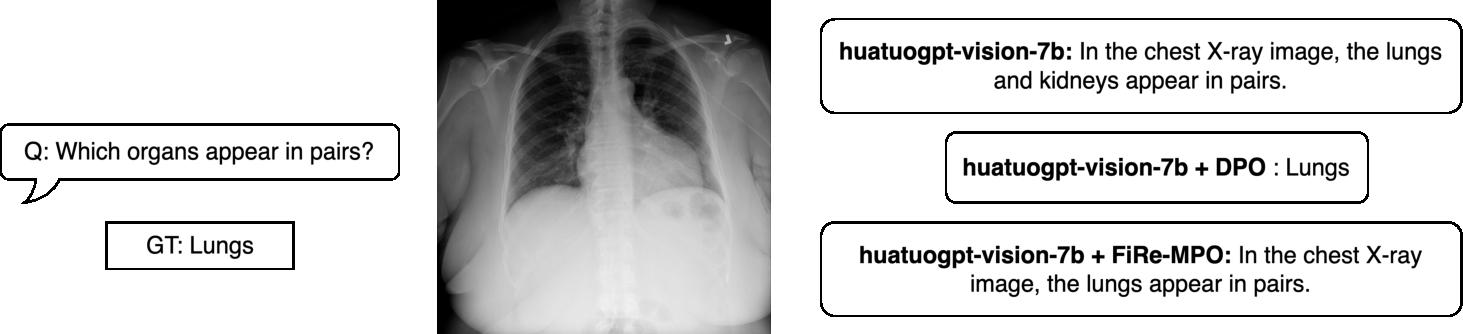
\includegraphics[width=\textwidth]{examples/example6.pdf}
    \caption{Qualitative comparison on anatomical localization (laterality).}
    \label{fig:case6}
\end{figure}

\begin{figure}[ht]
    \centering
    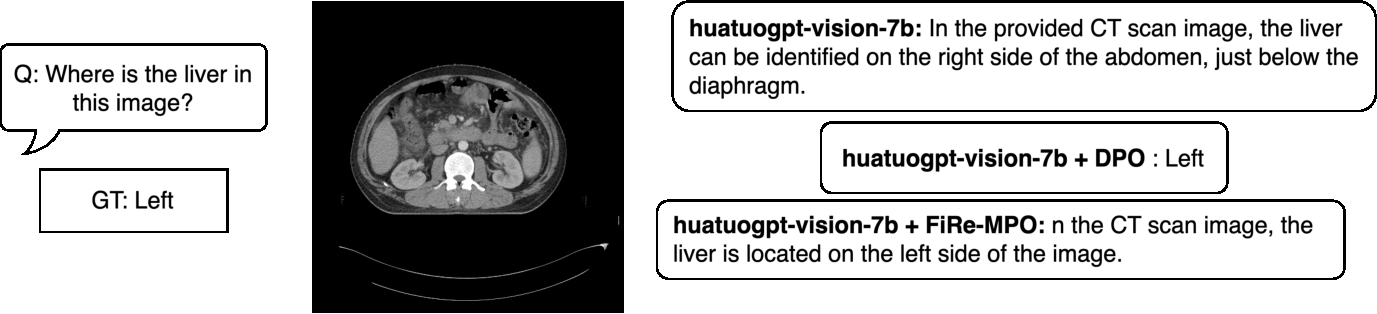
\includegraphics[width=\textwidth]{examples/example7.pdf}
    \caption{Additional qualitative comparison across backbones.}
    \label{fig:case7}
\end{figure}

\clearpage
\subsection{Reproduction Guide}
\label{app:repro}

Table~\ref{tab:repro} maps the components described in this thesis onto the accompanying code release, so that each equation, figure, and table can be traced to the code that produced it.

\begin{table}[ht]
\centering
\small
\caption{Mapping from thesis content to the code release.}
\label{tab:repro}
\begin{tabular}{ll}
\toprule
\textbf{Thesis content} & \textbf{Code} \\
\midrule
Eq.~\ref{eq:firempo-rank} (dual-constraint ranking loss) & \texttt{fire\_mpo/trainer/fire\_mpo\_trainer.py} \\
Eq.~\ref{eq:firempo-kl} (bidirectional token-wise KL) & \texttt{fire\_mpo/loss/fire\_mpo.py} \\
Eq.~\ref{eq:firempo-total} (complete objective) & \texttt{FiReMPOTrainer.get\_batch\_loss\_metrics} \\
\S\ref{sec:met:data} (on-policy preference construction) & \texttt{python -m fire\_mpo.pipeline.build\_text\_prefs} \\
\S\ref{sec:met:corruption} (lesion-targeted corruption) & \texttt{fire\_mpo.pipeline.enrich\_medsam3\_prompt} \\
 & then \texttt{fire\_mpo.pipeline.corrupt\_lesions} \\
Table~\ref{tab:hyperparams} (hyperparameters) & \texttt{configs/fire\_mpo\_default.yaml} \\
Tables~\ref{tab:regularizer}--\ref{tab:pair_ablation} (ablations) & \texttt{configs/ablations/} \\
RRPO baseline & same trainer, $\gamma = 0$, $\lambda = 1$ \\
MASK-DPO baseline & same trainer, $\gamma = 0$, $\alpha = 0$ \\
\S\ref{sec:res:main} (VQA accuracy) & \texttt{scripts/baselines/evaluation.sh} \\
\S\ref{sec:res:main} (GREEN score) & \texttt{scripts/baselines/green\_score.sh} \\
\S\ref{sec:res:grounding} (VGMED grounding) & \texttt{scripts/baselines/visual\_grounding.sh} \\
Figure~\ref{fig:training_dynamics} (training dynamics) & \texttt{thesis/images/new/make\_training\_dynamics.py} \\
\bottomrule
\end{tabular}
\end{table}

Because RRPO and MASK-DPO are configurations of the same trainer rather than separate codebases, the only baseline requiring its own implementation is mDPO, which adds a distinct conditional-preference term to the DPO loss.


\end{document}
